\documentclass[
twoside,
openright,
titlepage,
numbers=noenddot,
headinclude,%1headlines,
footinclude=true,
cleardoublepage=empty,
dottedtoc, % Make page numbers in the table of contents flushed right with dots leading to them
BCOR=5mm,
fontsize=10pt, % Binding correction, paper type and font size
ngerman,
american, % Languages, change this to your language(s)
pagesize=pdftex,
]{scrbook} 

%%%%%%%%%%%%%%%%%%%%%%%%%%%%%%%%%%%%%%%%%
% Classicthesis Typographic Thesis
% Configuration File
%
% This file has been downloaded from:
% http://www.LaTeXTemplates.com
%
% Original author:
% André Miede (http://www.miede.de) with extensive commenting changes by:
% Vel (vel@LaTeXTemplates.com)
%
% License:
% GNU General Public License (v2)
%
% Important note:
% The main lines to change in this file are in the DOCUMENT VARIABLES
% section, the rest of the file is for advanced configuration.
%
%%%%%%%%%%%%%%%%%%%%%%%%%%%%%%%%%%%%%%%%%

%----------------------------------------------------------------------------------------
%	CHARACTER ENCODING
%----------------------------------------------------------------------------------------

\PassOptionsToPackage{utf8}{inputenc} % Set the encoding of your files. UTF-8 is the only sensible encoding nowadays. If you can't read äöüßáéçèê∂åëæƒÏ€ then change the encoding setting in your editor, not the line below. If your editor does not support utf8 use another editor!
\usepackage{inputenc}
\usepackage{tabularx}

%----------------------------------------------------------------------------------------
%	DOCUMENT VARIABLES
%	Fill in the lines below to enter your information into the thesis template
%	Each of the commands can be cited anywhere in the thesis
%----------------------------------------------------------------------------------------

% Remove drafting to get rid of the '[ Date - classicthesis version 4.0 ]' text at the bottom of every page
\PassOptionsToPackage{listings, pdfspacing, subfig,beramono,parts}{classicthesis}
% Available options: drafting parts nochapters linedheaders eulerchapternumbers beramono eulermath pdfspacing minionprospacing tocaligned dottedtoc manychapters listings floatperchapter subfig

\newcommand{\myTitle}{A Classic Thesis Style\xspace}
\newcommand{\mySubtitle}{An Homage to The Elements of Typographic Style\xspace}
\newcommand{\myDegree}{Doktor-Ingenieur (Dr.-Ing.)\xspace}
\newcommand{\myName}{André Miede\xspace}
\newcommand{\myProf}{Put name here\xspace}
\newcommand{\myOtherProf}{Put name here\xspace}
\newcommand{\myFaculty}{Put data here\xspace}
\newcommand{\myDepartment}{Put data here\xspace}
\newcommand{\myUni}{Put data here\xspace}
\newcommand{\myLocation}{Saarbrücken\xspace}
\newcommand{\myTime}{September 2015\xspace}
\newcommand{\myVersion}{version 4.2\xspace}

%----------------------------------------------------------------------------------------
%	USEFUL COMMANDS
%----------------------------------------------------------------------------------------

\newcommand{\ie}{i.\,e.}
\newcommand{\Ie}{I.\,e.}
\newcommand{\eg}{e.\,g.}
\newcommand{\Eg}{E.\,g.} 

\newcounter{dummy} % Necessary for correct hyperlinks (to index, bib, etc.)
\providecommand{\mLyX}{L\kern-.1667em\lower.25em\hbox{Y}\kern-.125emX\@}
\newlength{\abcd} % for ab..z string length calculation

%----------------------------------------------------------------------------------------
%	PACKAGES
%----------------------------------------------------------------------------------------

%\PassOptionsToPackage{ngerman,american}{babel}  % Change this to your language(s)
% Spanish languages need extra options in order to work with this template
%\PassOptionsToPackage{spanish,es-lcroman}{babel}
\usepackage{babel}

\usepackage{lmodern} % text font
%------------------------------------------------			
\usepackage{makeidx}
\makeindex
%------------------------------------------------	
\usepackage{csquotes}
\PassOptionsToPackage{%
%backend=biber, % Instead of bibtex
backend=bibtex8,bibencoding=ascii,%
language=auto,%
style=numeric-comp,%
%style=authoryear-comp, % Author 1999, 2010
%bibstyle=authoryear,dashed=false, % dashed: substitute rep. author with ---
sorting=none, % name, year, title
maxbibnames=10, % default: 3, et al.
%backref=true,%
natbib=true % natbib compatibility mode (\citep and \citet still work)
}{biblatex}
\usepackage{biblatex}
 
 %------------------------------------------------

\PassOptionsToPackage{fleqn}{amsmath} % Math environments and more by the AMS 
 \usepackage{amsmath}

\DeclareMathOperator*{\argmax}{argmax}   % Jan Hlavacek
\DeclareMathOperator*{\argmin}{argmin}   % Jan Hlavacek
 
 %------------------------------------------------

\usepackage{amssymb} % The extended math symbols, e.g. lesssim and gtrsim
\usepackage{braket} % the braket
%------------------------------------------------

\PassOptionsToPackage{T1}{fontenc} % T2A for cyrillics
\usepackage{fontenc}

%------------------------------------------------

\usepackage{textcomp} % Fix warning with missing font shapes

%------------------------------------------------
\usepackage{epsdice} % dice symbols
\usepackage{marvosym} % boy, girl symbols
\usepackage{twemojis} % fruit symbols
%------------------------------------------------

\usepackage{scrhack} % Fix warnings when using KOMA with listings package  

%------------------------------------------------

\usepackage{xspace} % To get the spacing after macros right

%------------------------------------------------

\usepackage{mparhack} % To get marginpar right

%------------------------------------------------

\usepackage{fixltx2e} % Fixes some LaTeX stuff 

%------------------------------------------------
\usepackage{cancel} % for cancels to

%------------------------------------------------
\usepackage{amsthm} % For proofs among other things
\usepackage{float}

%------------------------------------------------
\PassOptionsToPackage{smaller}{acronym} % Include printonlyused in the first bracket to only show acronyms used in the text
\usepackage{acronym} % Nice macros for handling all acronyms in the thesis

%\renewcommand*{\acsfont}[1]{\textssc{#1}} % For MinionPro
\renewcommand*{\aclabelfont}[1]{\acsfont{#1}}


%------------------------------------------------

\PassOptionsToPackage{pdftex}{graphicx}
\usepackage{graphicx} 

%----------------------------------------------------------------------------------------
%	ENVIRONMENTS
%----------------------------------------------------------------------------------------

\newtheorem{axiom}{Axiom}
\newtheorem{definition}{Definition}
\newtheorem{theorem}{Theorem}
\newtheorem{corollary}{Corollary}
\newtheorem{exinn}{Example}[chapter]
\newenvironment{example}
{\clubpenalty=10000
	\begin{exinn}%
		\mbox{}%
		{\color{black}\leaders\hrule height .8ex depth \dimexpr-.8ex+0.8pt\relax\hfill}%
		\mbox{}\linebreak\ignorespaces}
	{\par\kern2ex\hrule\end{exinn}}

%----------------------------------------------------------------------------------------
%	FLOATS: TABLES, FIGURES AND CAPTIONS SETUP
%----------------------------------------------------------------------------------------

\usepackage{tabularx} % Better tables
\setlength{\extrarowheight}{3pt} % Increase table row height
\newcommand{\tableheadline}[1]{\multicolumn{1}{c}{\spacedlowsmallcaps{#1}}}
\newcommand{\myfloatalign}{\centering} % To be used with each float for alignment
\usepackage{caption}
\captionsetup{font=small}
\usepackage{subfig}  

%----------------------------------------------------------------------------------------
%	CODE LISTINGS SETUP
%----------------------------------------------------------------------------------------


\usepackage{xcolor} % Colors for Python environment

% Define colors for Python code syntax highlighting
\definecolor{RoyalBlue}{rgb}{0.25, 0.41, 0.88}
\definecolor{webgreen}{rgb}{0.0, 0.5, 0.0}
\definecolor{webbrown}{rgb}{0.65, 0.16, 0.16}
\definecolor{keywordcolor}{rgb}{0.5, 0, 0.5}
\definecolor{stringcolor}{rgb}{0.5, 0.5, 0}
\definecolor{commentcolor}{rgb}{0.25, 0.5, 0.35}
\definecolor{backgroundcolor}{rgb}{0.95, 0.95, 0.92}
\definecolor{Maroon}{rgb}{0.5, 0.0, 0.0}
\definecolor{Black}{rgb}{0.0, 0.0, 0.0}

\usepackage{algorithm}
\usepackage{algpseudocode}
\usepackage{pythonhighlight}



%----------------------------------------------------------------------------------------
%	HYPERREFERENCES
%----------------------------------------------------------------------------------------

\PassOptionsToPackage{pdftex,hyperfootnotes=false,pdfpagelabels}{hyperref}
\usepackage{hyperref}  % backref linktocpage pagebackref
\pdfcompresslevel=9
\pdfadjustspacing=1

\hypersetup{
% Uncomment the line below to remove all links (to references, figures, tables, etc), useful for b/w printouts
%draft, 
colorlinks=False,
linktocpage=true,
pdfstartpage=3,
pdfstartview=FitV,
% Uncomment the line below if you want to have black links (e.g. for printing black and white)
%colorlinks=false, linktocpage=false, pdfborder={0 0 0}, pdfstartpage=3, pdfstartview=FitV, 
breaklinks=true,
pdfpagemode=UseNone,
pageanchor=true,
pdfpagemode=UseOutlines,%
plainpages=false,
bookmarksnumbered,
bookmarksopen=true,
bookmarksopenlevel=1,%
hypertexnames=true,
pdfhighlight=/O,%nesting=true,%frenchlinks,%
urlcolor=webbrown,
linkcolor=RoyalBlue,
citecolor=webgreen,
%pagecolor=RoyalBlue,%
%urlcolor=Black, linkcolor=Black, citecolor=Black, %pagecolor=Black,%
%------------------------------------------------
% PDF file meta-information
pdftitle={\myTitle},
pdfauthor={\textcopyright\ \myName, \myUni, \myFaculty},
pdfsubject={},
pdfkeywords={},
pdfcreator={pdfLaTeX},
pdfproducer={LaTeX with hyperref and classicthesis}
%------------------------------------------------
}

%----------------------------------------------------------------------------------------
%	AUTOREFERENCES SETUP
%	Redefines how references in text are prefaced for different 
%	languages (e.g. "Section 1.2" or "section 1.2")
%----------------------------------------------------------------------------------------

\makeatletter
\@ifpackageloaded{babel}
{
\addto\extrasamerican{
\renewcommand*{\figureautorefname}{Figure}
\renewcommand*{\tableautorefname}{Table}
\renewcommand*{\partautorefname}{Part}
\renewcommand*{\chapterautorefname}{Chapter}
\renewcommand*{\sectionautorefname}{Section}
\renewcommand*{\subsectionautorefname}{Section}
\renewcommand*{\subsubsectionautorefname}{Section}
}
\addto\extrasngerman{
\renewcommand*{\paragraphautorefname}{Absatz}
\renewcommand*{\subparagraphautorefname}{Unterabsatz}
\renewcommand*{\footnoteautorefname}{Fu\"snote}
\renewcommand*{\FancyVerbLineautorefname}{Zeile}
\renewcommand*{\theoremautorefname}{Theorem}
\renewcommand*{\appendixautorefname}{Anhang}
\renewcommand*{\equationautorefname}{Gleichung}
\renewcommand*{\itemautorefname}{Punkt}
}
\providecommand{\subfigureautorefname}{\figureautorefname} % Fix to getting autorefs for subfigures right
}{\relax}
\makeatother

%----------------------------------------------------------------------------------------

\usepackage{classicthesis} 

%----------------------------------------------------------------------------------------
%	CHANGING TEXT AREA 
%----------------------------------------------------------------------------------------

%\linespread{1.05} % a bit more for Palatino
%\areaset[current]{280pt}{600pt} % 686 (factor 2.2) + 33 head + 42 head \the\footskip
%\setlength{\marginparwidth}{7em}%
%\setlength{\marginparsep}{2em}%
\usepackage[a4paper,margin=1in]{geometry}

%----------------------------------------------------------------------------------------
%	USING DIFFERENT FONTS
%----------------------------------------------------------------------------------------

%\usepackage[oldstylenums]{kpfonts} % oldstyle notextcomp
%\usepackage[osf]{libertine}
%\usepackage[light,condensed,math]{iwona}
%\renewcommand{\sfdefault}{iwona}
%\usepackage{lmodern} % <-- no osf support :-(
%\usepackage{cfr-lm} % 
%\usepackage[urw-garamond]{mathdesign} <-- no osf support :-(
%\usepackage[default,osfigures]{opensans} % scale=0.95 
%\usepackage[sfdefault]{FiraSans}

%----------------------------------------------------------------------------------------
%	Including pdf's
%----------------------------------------------------------------------------------------
\usepackage{pdfpages}
\addbibresource{refs.bib} % The file housing your bibliography

\begin{document}
	\frenchspacing % Reduces space after periods to make text more compact
	\raggedbottom % Makes all pages the height of the text on that page
	\selectlanguage{american} % Select your default language - e.g. american or ngerman
	\pagenumbering{roman} % Roman page numbering prior to the start of the thesis content (i, ii, iii, etc)
	
	\pagestyle{plain} % Suppress headers for the pre-content pages
	
	%----------------------------------------------------------------------------------------
	%	PRE-CONTENT THESIS PAGES
	%----------------------------------------------------------------------------------------
	
	% Title Page

\begin{titlepage}


\begin{center}
\large

\hfill
\bigskip\bigskip

\begingroup
\spacedallcaps{Introduction to Statistics} \\ \bigskip
\endgroup

\spacedlowsmallcaps{Theory, Methods, and Applications} \\ \bigskip\bigskip\bigskip\bigskip

\spacedlowsmallcaps{Authored by} \\ \medskip

\spacedallcaps{ Jonas Petersen} \\



\today








\end{center}


\end{titlepage} % Main title page
	% Back of the title page

\thispagestyle{empty}

\hfill

\vfill

This page is intentionally left blank

\vfill

% You may wish to do something with the back of the title page, such as including your supervisors, location or time frame of the work. Below is an example of doing so although you may want to tweak it to your liking.

%\bigskip

%\noindent\spacedlowsmallcaps{Supervisors}: \\
%\myProf \\
%\myOtherProf \\ 
%\mySupervisor

%\medskip \\

%\noindent\spacedlowsmallcaps{Location}: \\
%\myLocation

%\medskip \\

%\noindent\spacedlowsmallcaps{Time Frame}: \\
%\myTime
 % Back of the title page
	
	\pagestyle{scrheadings} % Show chapter titles as headings
	
	\tableofcontents
	\cleardoublepage
	\pagenumbering{arabic} % Arabic page numbering for thesis content (1, 2, 3, etc)
	\cleardoublepage % Avoids problems with pdfbookmark
	
	%----------------------------------------------------------------------------------------
	%	THESIS CONTENT - CHAPTERS
	%----------------------------------------------------------------------------------------
	
	\chapter{Preface}
\label{chp:preface}
Statistics is a mathematical discipline that use probability theory (which in turn require set theory) to extract insights from information (data). Probability theory is a branch of pure mathematics -- probabilistic questions can be posed and solved using axiomatic reasoning, and therefore there is one correct answer to any probability question. Statistical questions can be converted to probability questions by the use of probability models. Given certain assumptions about the mechanism generating the data, statistical questions can be answered using probability theory. This highlights the dual nature of statistics, comprised of two integral parts.
\begin{enumerate}
	\item The first part involves the formulation and evaluation of probabilistic models, a process situated within the realm of the philosophy of science. This phase grapples with the foundational aspects of constructing models that accurately represent the problem at hand.
	\item The second part concerns itself with extracting answers after assuming a specific model. Here, statistics becomes a practical application of probability theory, involving not only theoretical considerations but also numerical analysis in real-world scenarios.
\end{enumerate}
This duality underscores the interdisciplinary nature of statistics, bridging the gap between the conceptual and the applied aspects of probability theory. Although probabilities are well defined (see \chref{chp:probaiblity_theory}), their interpretation is not defined beyond their definition. This ambiguity has given birth to two competing interpretations of probability, leading to two competing branches of statistics; Frequentist and Bayesian Statistics. This book aims to explain how these competing branches of statistics fit together as well as providing a non-exhaustive presentation of some of the methods within both branches. The philosophy of the book is rather straight to the point, but with a lot of examples both big and small. Some of these are anonymized versions of projects from industry. The books is split into three parts; introduction (Part \ref{part:introduction}), Frequentist statistics (Part \ref{part:frequentist}) and Bayesian statistics (Part \ref{part:bayesian}). 


\section{Acknowledgements}
The philosophy of the book is similar to \cite{Sivia2006}, a few exercises from \cite{murphy2023probabilistic} used as examples, the idea of phrasing decision theory as "Robot vs Nature" from \cite{lavalle2006planning} and the review of probability theory is inspired by \cite{chan2021introduction}.
	
	\part{Introduction}
	\label{part:introduction}
	\chapter{Introduction to Set Theory}
\label{chp:set_theory}
Set theory is a fundamental branch of mathematical logic that provides a foundation for much of mathematics, including probability theory. At its core, set theory deals with the concept of a set, which is a collection of distinct objects or elements. In this introduction, the essential properties and operations of sets are explored in order to lay the groundwork for the axiomatic formation of probability theory and statistics.


\begin{definition}[Membership]
	In set theory, the membership relation between an object $o$ and a set $A$ is fundamental. $o \in A$ denotes that $o$ is an element or member of $A$.
\end{definition}

\begin{definition}[Set]
	A set is a collection of distinct objects, considered as an object in its own right. Sets are typically denoted using curly braces $\{\}$ and can be described in two primary ways:
	\begin{enumerate}
		\item By listing its elements separated by commas, e.g., $A = \{a_1, a_2, a_3\}$.
		\item By specifying a characterizing property of its elements, e.g., $A = \{x \mid x \text{ is a natural number}\}$.
	\end{enumerate}
	Sets can also be illustrated graphically, as shown in \figref{fig:generic_set}.
	\begin{figure}[H]
		\centering
		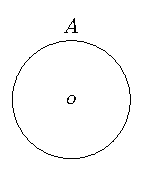
\includegraphics[width = 0.3\textwidth]{figures/generic_set.pdf}
		\caption{The graphical representation of a generic set $A$ with generic elements $o$.}
		\label{fig:generic_set}
	\end{figure}
\end{definition}

\begin{definition}[Subset]
	A set $A$ is called a subset of a set $B$, denoted $A \subseteq B$, if every element of $A$ is also an element of $B$. Formally, $A\subseteq B$ if $\forall x \in A, x \in B$. By this definition, a set is always a subset of itself.
	\begin{figure}[H]
		\centering
		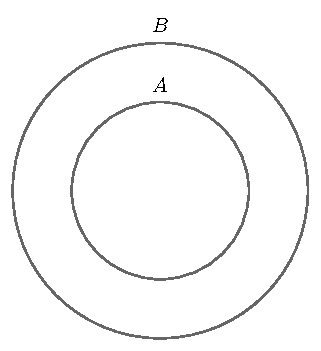
\includegraphics[width = 0.5\textwidth]{figures/set_subset.pdf}
		\caption{The graphical representation of $A\subseteq B$.}
		\label{fig:set_subset}
	\end{figure}
\end{definition}

\begin{definition}[Proper Subset]
	A set $A$ is called a proper subset of a set $B$, denoted $A \subset B$, if $A \subseteq B$ and $A \neq B$. This means that $A$ is a subset of $B$ but $A$ is not equal to $B$; there is at least one element in $B$ that is not in $A$.
\end{definition}

\begin{example}
	Suppose $A = \{\twemoji{banana}, \twemoji{apple}, \twemoji{eggplant}\}$, then $\{\twemoji{banana}, \twemoji{apple}\}$ and $\{\twemoji{apple}\}$ are proper subsets of $A$, meaning $\{\twemoji{banana}, \twemoji{apple}\},\{\twemoji{apple}\}\subset  A$. $\{\twemoji{banana}, \twemoji{carrot}\}$, on the other hand, is not a subset of $A$, meaning $\{\twemoji{banana}, \twemoji{carrot}\}\not\subset  A$.
\end{example}
\begin{example}
	$\twemoji{banana}$, $\twemoji{apple}$, and $\twemoji{eggplant}$ are members (elements) of the set $\{\twemoji{banana}, \twemoji{apple}, \twemoji{eggplant}\}$, but are not subsets of it; and in turn, the subsets, such as $\{\twemoji{banana}\}$, are not members of the set $\{\twemoji{banana}, \twemoji{apple}, \twemoji{eggplant}\}$.
\end{example}

\begin{definition}[Empty Set]
	The empty set, denoted by $\emptyset$ or $\{\}$, is the set that contains no elements.
\end{definition}

\begin{definition}[Universal Set]
	The universal set, denoted by $\Omega$, is the set that contains all the objects or elements under consideration in a particular discussion or problem. It is the largest set in the context of a given study.
\end{definition}

\begin{definition}[Closure]
	A set $A$ is said to be \textit{closed} under a certain operation if, for every pair of elements $x$ and $y$ in $A$, the result of applying the operation to $x$ and $y$ is also in $A$.
\end{definition}

\begin{definition}[Union]
	The union of sets $A$ and $B$, denoted by $A \cup B$, is defined as the set containing all elements that are in $A$ or $B$ (or both). \figref{fig:set_union} provide a graphical representation of $A \cup B$.
	\begin{figure}[h]
		\centering
		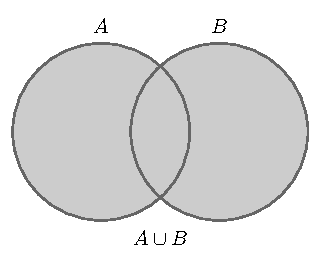
\includegraphics[width = 0.6\textwidth]{figures/set_union.pdf}
		\caption{The figure show the union of sets $A$ and $B$. Each circle represent the sets and the colored region represent the result of the result of the binary operation.}
		\label{fig:set_union}
	\end{figure}
\end{definition}

\begin{definition}[Intersection]
	The intersection of sets $A$ and $B$, denoted by $A \cap B$, is defined as the set containing all elements that are common to both $A$ and $B$. \figref{fig:set_intersection} provide a graphical representation of $A \cap B$.
	\begin{figure}[H]
		\centering
		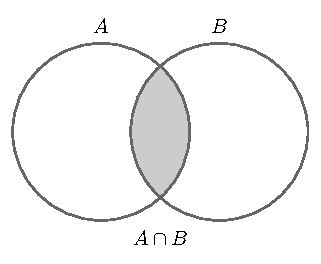
\includegraphics[width = 0.6\textwidth]{figures/set_intersection.pdf}
		\caption{The figure show the intersection of sets $A$ and $B$. Each circle represent the sets and the colored region represent the result of the result of the binary operation.}
		\label{fig:set_intersection}
	\end{figure}
\end{definition}

\begin{definition}[Disjoint]
	Two sets $A$ and $B$ are said to be disjoint if their intersection is the empty set, i.e., $A \cap B = \emptyset$. \figref{fig:set_disjoint} provide a graphical representation of $A \cap B=\emptyset$.
	\begin{figure}[H]
		\centering
		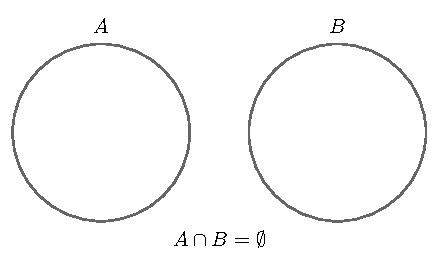
\includegraphics[width = 0.8\textwidth]{figures/set_disjoint.pdf}
		\caption{The figure show the case where the intersection of sets $A$ and $B$ is the empty set. Each circle represent the sets and the colored region represent the result of the result of the binary operation.}
		\label{fig:set_disjoint}
	\end{figure}
\end{definition}


\begin{definition}[Complementation]
	The complement of set $A$, denoted by $A^c$, is defined as the set containing all elements in the universal set $\Omega$ that are not in $A$. \figref{fig:set_complementation} provide a graphical representation of $(A \cap B)^c$.
	\begin{figure}[H]
		\centering
		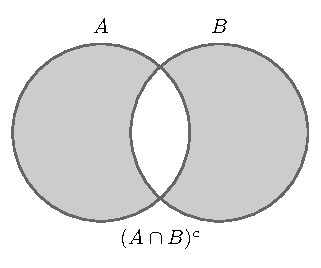
\includegraphics[width = 0.6\textwidth]{figures/set_complementary.pdf}
		\caption{The figure show the complementary of the intersection of sets $A$ and $B$. Each circle represent the sets and the colored region represent the result of the result of the binary operation.}
		\label{fig:set_complementation}
	\end{figure}
\end{definition}

\begin{definition}[Difference]
	The difference between set $A$ and $B$, denoted by $A \setminus B = A\cap B^c$, is defined as the set containing all elements in $A$ that are not in $B$. \figref{fig:set_minus} provide a graphical representation of $A\setminus B$ and $B\setminus A$.
	\begin{figure}[H]
		\centering
		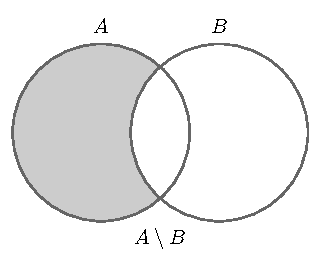
\includegraphics[width = 0.6\textwidth]{figures/set_minus.pdf}
		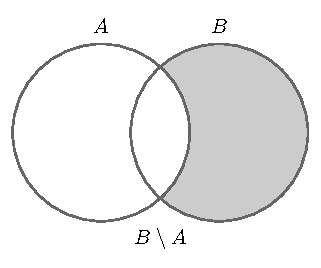
\includegraphics[width = 0.6\textwidth]{figures/set_minus2.pdf}
		\caption{(left) show $A$ minus $B$ and (right) show $B$ minus $A$. Each circle represent the sets and the colored region represent the result of the result of the binary operation.}
		\label{fig:set_minus}
	\end{figure}
\end{definition}

\begin{definition}[Power Set]
	The power set of a set $A$, denoted by $2^A$, is defined as the set containing all possible subsets of $A$, including $A$ itself and the empty set.
\end{definition}

\begin{example}
	Suppose $A = \{a_1,a_2,a_3\}$, then
	\begin{equation}
		\begin{split}
			2^A = \{&\emptyset, \{a_1\}, \{a_2\}, \{a_3\}, \{a_1, a_2\},\\
			& \{a_1, a_3\}, \{a_2, a_3\}, \{a_1, a_2, a_3\}\}.
		\end{split}
	\end{equation}
\end{example}

\begin{definition}[Symmetric Difference]
	The symmetric difference of sets $A$ and $B$, denoted by $A \Delta B$, is defined as the set containing all elements that are in either $A$ or $B$ but not in both, meaning $A \Delta B = (A \cap B)^c$. \figref{fig:set_complementation} show the symmetric difference between sets $A$ and $B$.
\end{definition}

\begin{definition}[Finite and Infinite Unions]
	For a collection $\{A_i\}$, the union is denoted by $\bigcup_{i} A_i$ and is defined as the set containing all elements that are in at least one of the sets $A_i$.
\end{definition}

\begin{definition}[Partition]
	A collection of non-empty subsets $\{A_i\}$ of a set $A$ is called a partition of $A$ if the following conditions are satisfied:
	\begin{enumerate}
		\item The subsets $A$ are pairwise disjoint, i.e., $A_i \cap A_j = \emptyset$ for all \(i \neq j\).
		\item The union of all subsets \(A_i\) is equal to the set \(A\), i.e., \(\bigcup_{i \in I} A_i = A\).
	\end{enumerate}
	
	A graphical representation of the set $A=\{A_1,A_2,A_3\}$, where $A_j$ are partitions, is shown in \figref{fig:set_partition}.
	\begin{figure}[h]
		\centering
		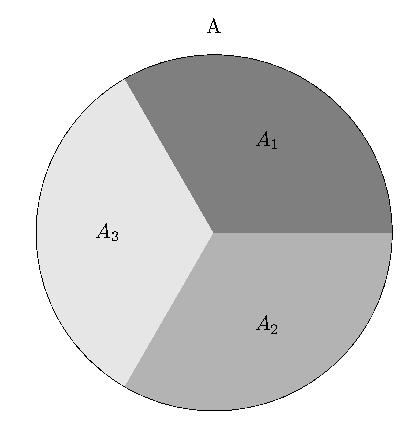
\includegraphics[width = 0.6\textwidth]{figures/set_partition.pdf}
		\caption{The figure show $A=\{A_1,A_2,A_3\}$ where $A_j$ are partitions.}
		\label{fig:set_partition}
	\end{figure}
\end{definition}


\begin{definition}[Finite and Infinite Intersections]
	For a collection $\{A_i\}$, the intersection is denoted by $\bigcap_{i} A_i$ and is defined as the set containing all elements that are common to all sets $A_i$.
\end{definition}

\begin{definition}[Cartesian Product]
	The Cartesian product of sets $A$ and $B$, denoted by $A \times B$, is defined as the set containing all ordered pairs $(a, b)$, where $a$ is in $A$ and $b$ is in $B$.
\end{definition}

\begin{example}
	Suppose $A= \{a_1,a_2\}$ and $B=\{b_1,b_2,b_3\}$, then
	\begin{equation}
		\begin{split}
			A\times B = \{&(a_1,b_1),(a_1,b_2),(a_1,b_3),\\
			&(a_2,b_1),(a_2,b_2),(a_2,b_3)\}
		\end{split}
	\end{equation}
\end{example}

	

	\chapter{Introduction to Probability Theory}
\label{chp:probaiblity_theory}
Probability theory aims to provide a mathematical framework for analyzing random experiments, where outcomes cannot be predicted with certainty beforehand. Its objective is to systematically study and understand the potential outcomes of these experiments. 
\begin{definition}[Sample Space]
	The sample space, denoted by \( \Omega \), represents the set of all possible outcomes of a random experiment. It encompasses every conceivable result that could occur, serving as the foundation for analyzing probabilities associated with different outcomes.
\end{definition}

\begin{definition}[Event]
	An event, $E$, is a subset of the sample space, denoted by $E \subseteq \Omega$, that corresponds to a specific collection of possible outcomes in a random experiment. Events may consist of single or multiple outcomes and are defined by the occurrence or non-occurrence of particular conditions.
\end{definition}

\begin{example}
	\label{ex:die1}
	Consider the roll of a fair six-sided die. The sample space for this experiment is given by $\Omega = \{ \epsdice{1}, \epsdice{2}, \epsdice{3}, \epsdice{4}, \epsdice{5}, \epsdice{6} \}$. $E = \{\epsdice{2}, \epsdice{4}, \epsdice{6}\}$, is the event of rolling an even number. 
\end{example}

\begin{definition}[Event Space]
	The set containing all valid possible events for a random experiment is referred to as the event space, $\mathcal{F}$. The notion of "all valid possible events for a random experiment" is formally defined by requiring $\mathcal{F}$ to be a $\sigma$-algebra satisfying the following properties:
	\begin{enumerate}
		\item $\mathcal{F}$ is the set of all subsets of the sample space $\Omega$, including the empty set $\emptyset$ and $\Omega$ itself, along with various combinations of outcomes.
		\item Closure under complementation: If $E$ is in the $\sigma$-algebra ($E \in \mathcal{F}$), then its complement $E^c$ is also in the $\sigma$-algebra.
		\item Closure under countable union and intersection: If the events $E_1, E_2, E_3, \dots$ are in the $\sigma$-algebra ($E_i \in \mathcal{F}$ for all $i$), then their countable union $\bigcup_{i=1}^{\infty} E_i$ and intersection $\bigcap_{i=1}^{\infty} E_i$ are also in the $\sigma$-algebra.
	\end{enumerate}
	In the case where the outcomes of the random experiment can take discrete values, these properties are sufficient. However, in the case where the outcomes are continuous, $\mathcal{F}$ is required to be a Borel $\sigma$-algebra, meaning it must further fulfill the closure property under countable intersection with open sets. This ensures that $\mathcal{F}$ contains all sets that can be formed by taking unions, intersections, and complements of open sets, which are essential for defining probabilities in continuous spaces.
\end{definition}


\begin{example}
	\label{ex:die2}
	For the roll with the fair die considered in \exref{ex:die1}, the sample space is $\Omega = \{ \epsdice{1}, \epsdice{2}, \epsdice{3}, \epsdice{4}, \epsdice{5}, \epsdice{6} \}$ and the event space (the set of all possible events) is given by
	\begin{equation}
		\begin{split}
			\mathcal{F}&=\{\emptyset, \{\epsdice{1}\},\{\epsdice{1},\epsdice{3}\},\{\epsdice{3}\},\{\epsdice{1},\epsdice{2},\epsdice{3},\epsdice{4}\},\{\epsdice{5}\},\dots\}\\
			& = 2^\Omega.
		\end{split}
	\end{equation}
\end{example}

\begin{definition}[Measurable Space]
	\label{def:measurable_space}
	The pair \( (\Omega, \mathcal{F}) \) is called a measurable space.
\end{definition}

Probability can loosely be defined~\cite{chan2021introduction} as a measure of the size of an event (a set) relative to the sample space (another set), meaning it is a function that operates on an event (a set). In particular the probability measure maps any valid event, i.e. any $E\in \mathcal{F}$, to a number between $0$ and $1$, representing the relative size of the event to the sample space.

\begin{definition}[Probability Measure]
	\label{def:probability}
	A Probability measure\index{Probability Measure}, $\mathbb{P}$, is a set function \index{Set function} defined on a measurable space (\dfref{def:measurable_space}) $(\Omega, \mathcal{F})$
	\begin{equation}
		\mathbb{P}: \mathcal{F} \mapsto [0,1]
	\end{equation}
	that obey~\cite{kolmogorov1950foundations} \axref{ax:non_neg}-\axref{ax:add}\index{Axioms of probability theory}.
\end{definition}

\begin{axiom}[Non-negativity]
	\label{ax:non_neg}
	For any event $E\in \mathcal{F}$, the probability measure $\mathbb{P}(E)$ is non-negative, satisfying
	\begin{equation}
		\mathbb{P}(E) \geq 0 \quad \forall E \in  \mathcal{F}.
	\end{equation}
\end{axiom}

\begin{axiom}[Normalization]
	\label{ax:norm}
	The probability of the universal set $\Omega$ is 1, satisfying
	\begin{equation}
		\mathbb{P}(\Omega) = 1.
	\end{equation}
\end{axiom}

\begin{axiom}[Additivity]
	\label{ax:add}
	For any countable sequence of mutually exclusive events $\mathit{E}_1, \mathit{E}_2, \ldots\in \mathcal{F}$, the probability of their union is the sum of their individual probabilities, such that
	\begin{equation}
		\mathbb{P}\left(\bigcup_{i=1}^{\infty} \mathit{E}_i\right) = \sum_{i=1}^{\infty} \mathbb{P}(\mathit{E}_i) \quad \forall \mathit{E}_i \in \mathcal{F} \text{ where } \bigcap_{i=1}^{\infty} \mathit{E}_i = \emptyset.
	\end{equation}
\end{axiom}
Together, the probability measure, the sample space and the algebra form the tuple $(\Omega, \mathcal{F}, \mathbb{P})$ which define what a probability space\index{Probability space}. The non-negativity and normalization axioms are largely matters of convention, although it is non-trivial that probability measures take at least the two values $0$ and $1$, and that they have a maximal value (unlike various other measures, such as length, volume, and so on, which are unbounded). The axioms are supplemented by two definitions.

\begin{definition}[Conditional Probability]
	\label{def:conditional_probability}
	For events $E_1$ and $E_2$ in a probability space $(\Omega, \mathcal{F}, \mathbb{P})$ with $\mathbb{P}(E_2) > 0$, the conditional probability\index{Conditional probability} of $E_1$ given $E_2$ is defined viz
	\begin{equation}
		\mathbb{P}(E_1|E_2) \equiv \frac{\mathbb{P}(E_1, E_2)}{\mathbb{P}(E_2)},
		\label{eq:cond}
	\end{equation}
	where $\mathbb{P}(E_1,E_2)= \mathbb{P}(E_1\cap E_2)$ to ease the notation.
\end{definition}
\begin{definition}[Independence]
	\label{def:independence}
	Events $E_1$ and $E_2$  in a probability space $(\Omega, \mathcal{F}, \mathbb{P})$ are said to be conditionally independent if
	\begin{equation}
		\mathbb{P}(E_1,E_2) = \mathbb{P}(E_1) \mathbb{P}(E_2).
		\label{eq:ind}
	\end{equation}
\end{definition}


From \axref{ax:non_neg}-\axref{ax:add}, \dfref{eq:cond} and \dfref{eq:ind}, the chain rule, the concept of marginalization, conditional independence and the law of total probability can be derived. 
\begin{theorem}[Chain Rule]
	\label{theorem:chain_rule}
	Given $\{E_1, E_2, \ldots, E_n\}\subseteq \mathcal{F}$ denotes a set of events in a probability space $(\Omega, \mathcal{F}, \mathbb{P})$, the chain rule\index{Chain rule} for this set of events can be written
	\begin{equation}
		\begin{split}
			\mathbb{P}(E_1, \dots E_n) = \mathbb{P}(E_1)\prod_{j=2}^{n}\mathbb{P}(E_j|E_1,\dots E_{j-1}).
		\end{split}
		\label{eq:prod}
	\end{equation}
\end{theorem}
\begin{proof}
	From the definition of conditional probability in \EQref{eq:cond}
	\begin{equation}
		\mathbb{P}(E_1, E_2, \ldots, E_n) = \mathbb{P}(E_1|E_2, \dots, E_n)\mathbb{P}(E_2, \dots, E_n).
		\label{eq:p1}
	\end{equation}
	Using the definition of conditional probability again
	\begin{equation}
		\mathbb{P}(E_2, \ldots, E_n) = \mathbb{P}(E_2| \ldots, E_n)\mathbb{P}(\dots, E_n).
	\end{equation}
	Continuing in this way, \EQref{eq:prod} follows.
\end{proof}
\EQref{eq:prod} illustrates how to decompose the joint probability of multiple events into a product of conditional probabilities. The idea is to calculate the probability of each event in the sequence conditioned on the occurrence of the previous events in the chain. The chain rule is particularly powerful when dealing with complex systems where events may be interdependent. It allows breaking down joint probabilities into more manageable conditional probabilities, making it easier to analyze and model intricate relationships between events. Whether in the context of statistical modeling or machine learning, the chain rule plays a key role in calculating the joint probability of multiple events and provides a foundation for more advanced probabilistic reasoning.

\begin{theorem}[Bayes theorem]
	\label{theorem:bayes_theorem}
	For events $E_1,E_2,E_3 \in \mathcal{F}$ in a probability space $(\Omega, \mathcal{F}, \mathbb{P})$, Bayes theorem\index{Bayes theorem} can be formulated viz
	\begin{equation}
		\mathbb{P}(E_1| E_2,E_3) = \frac{\mathbb{P}(E_2| E_1,E_3)\mathbb{P}(E_1,E_2)}{\mathbb{P}(E_2,E_3)}.
		\label{bayes_theorem}
	\end{equation}
\end{theorem}

\begin{proof}
	Bayes theorem follows directly from applying the chain rule and applying the concept of symmetry viz
	\begin{equation}
		\begin{split}
			\mathbb{P}(E_1,E_2,E_3) &= \mathbb{P}(E_1| E_2,E_3)\mathbb{P}(E_2,E_3) \\
			& = \mathbb{P}(E_2|E_1,E_3)\mathbb{P}(E_1,E_3)
		\end{split}
		\label{eq:c2}
	\end{equation}
	from which
	\begin{equation}
		\mathbb{P}(E_1| E_2,E_3) = \frac{\mathbb{P}(E_2| E_1,E_3)\mathbb{P}(E_1,E_2)}{\mathbb{P}(E_2,E_3)}
	\end{equation}
	which is Bayes theorem.
\end{proof}


\begin{theorem}[Law of Total Probability]
	\label{theorem:law_of_total_probability}
	Let $\{E_1,E_2,\dots E_n\}$ be a partition\index{Marginalization}\index{Law of Total Probability} of the sample space $\Omega$ of the probability space $(\Omega, \mathcal{F}, \mathbb{P})$, then for any $A\subseteq \Omega$,
	\begin{equation}
		\mathbb{P}(A) = \sum_{i} \mathbb{P}(A,E_i).
		\label{eq:marg}
	\end{equation}
	In continuous cases, the summation is replaced by integration.
\end{theorem}

\begin{proof}
	Consider an event $A\subseteq \Omega$ and a partition $\{E_1,E_2,\dots E_n\}$ of $\Omega$ such that $\cup_{i}E_i=\Omega$. For mutually exclusive events (which a partition by definition is), finite additivity can be used such that
	\begin{equation}
		\sum_{i}\mathbb{P}(A,E_i) = \mathbb{P}(\bigcup_{i}(A,E_i)).
		\label{eq:qq1}
	\end{equation} 
	$\bigcup_{i}(A,E_i)$ is the union of all intersections between $A$ and the $E$'s. However, since the $E$'s form a partition of $\Omega$, they together form $\Omega$ and the intersection between $\Omega$ and $A$ is $A$, meaning
	\begin{equation}
		\begin{split}
			\bigcup_{i}(A,E_i)  &= (A,\bigcup_{i}E_i)\\
			&= (A,\Omega)\\
			& =A.
		\end{split}
	\label{eq:qq2}
	\end{equation}
	Combining \EQref{eq:qq1}-\EQref{eq:qq2} then yields
	\begin{equation}
		\mathbb{P}(A) = \sum_{i} \mathbb{P}(A, E_i).
	\end{equation}
	
\end{proof}

\begin{example}
	Consider the roll of a fair six-sided die. The sample space for this experiment is given by $\Omega = \{ \epsdice{1}, \epsdice{2}, \epsdice{3}, \epsdice{4}, \epsdice{5}, \epsdice{6} \}$. Let $E_1 = \{\epsdice{2}, \epsdice{4}, \epsdice{6}\}$ and $E_2 = \{\epsdice{4}\}$ be two events, then from \EQref{eq:cond}
	\begin{equation}
		\begin{split}
			\mathbb{P}(E_1|E_2) &= \frac{\mathbb{P}(E_1, E_2)}{\mathbb{P}(E_2)}\\
			& = 1
		\end{split}
	\end{equation}
	where $\mathbb{P}(E_1,E_2)= \frac{1}{6}$ since $E_1,E_2 = E_1\cap E_2 = E_2=\{\epsdice{4}\}$ is one of $6$ possible values and $\mathbb{P}(E_2) = \frac{1}{6}$. Intuitively this makes sense because $E_2$ is a set with one member and since $E_2$ is known, the outcome of the experiment is known with certainty in this case.
\end{example}

\begin{definition}[Random Variable]
	\label{def:random_Variable}
	A random variable $X$ is a function 
	\begin{equation}
		X: \Omega \mapsto \Omega_X
	\end{equation}
	that maps outcomes from a probability space $(\Omega, \mathcal{F}, \mathbb{P})$ to a measurable space $(\Omega_X, \mathcal{F}_X)$, where $\Omega_X$ is the codomain of $X$ and $\mathcal{F}_X$ is a $\sigma$-algebra on $\Omega_X$. The $\sigma$-algebra $\mathcal{F}_X$ ensures that $X$ is measurable, meaning that for any set $x \in \mathcal{F}_X$, the preimage $X^{-1}(x)$ must belong to $\mathcal{F}$. Formally, this can be written as
	\begin{equation}
		X^{-1}(x) = \{\omega \in \Omega | X(\omega) = x\} \in \mathcal{F} \quad \forall x \in \mathcal{F}_X.
	\end{equation}
	Random variables are classified as either discrete or continuous, based on the discrete or continuous nature of their sample space. Discrete random variables have countable sample spaces, while continuous random variables have uncountable sample spaces, often modeled as intervals on the real line. The role of random variables is to provide a numerical representation of the outcomes of a random experiment, allowing quantification and analysis of the likelihood of different numerical outcomes. 
\end{definition}

\begin{definition}[Expected value]
	\label{def:expectation}
	Let $X$ be a real-valued random variable defined on a probability space $(\Omega, \mathcal{F},\mathbb{P})$, then the expected valued of $X$, denoted by $\mathbb{E}[X]$, is defined by the Lebesgue integral~\citep{taboga2021}
	\begin{equation}
		\mathbb{E}_X[X]\equiv \int _\Omega X(\omega)d\mathbb{P}(\{\omega\}).
		\label{eq:expected_value}
	\end{equation}
\end{definition}
\begin{theorem}[Non-negativity of expected value]
	If $X\geq 0$ for a random variable $X$, then $\mathbb{E}_X[X]\geq 0$.
\end{theorem}
\begin{theorem}[Linearity of expected value]
	The expectation is a linear operator meaning $\mathbb{E}_X[a+X] = a+\mathbb{E}_X[X]$ and $\mathbb{E}_X[aX] = a\mathbb{E}_X[X]$ for any constant $a$.
\end{theorem}
\begin{theorem}[The law of the unconscious statistician]
	The law of the unconscious statistician generalize the expectation of a random variable to the expectation of a function $g: \Omega \mapsto \mathbb{R}$ of a random variable $X(\omega)\in \Omega_X\quad \forall \omega \in \Omega$ defined on a probability space $(\Omega, \mathcal{F},\mathbb{P})$ such that
	\begin{equation}
		\mathbb{E}[g(X)]\equiv \int _\Omega g(X(\omega))d\mathbb{P}(\{\omega\}).
		\label{eq:expected_value2}
	\end{equation}
\end{theorem}

\begin{definition}[Variance]
	\label{def:variance}
	Let $X$ be a real-valued random variable defined on a probability space $(\Omega, \mathcal{F},\mathbb{P})$, then the variance of $X$, denoted by $\text{Var}[X]$, is defined viz
	\begin{equation}
		\begin{split}
			\text{Var}[X]&\equiv \mathbb{E}_X[(X-\mathbb{E}_X[X])^2]\\
			&= \mathbb{E}_X[X^2]-\mathbb{E}_X[X]^2.
		\end{split}
	\end{equation}
\end{definition}
\begin{theorem}[Non-linearity of variance]
	The variance is a non-linear opeator, where $Var[a+X]=Var[X]$ and $Var[aX]=a^2Var[X]$ for any constant $a$.
\end{theorem}


\begin{definition}[Image Measure]
	\label{def:image_measure}
	Let $X: \Omega \mapsto \Omega_X$ be a random variable that maps from the probability space $(\Omega, \mathcal{F}, \mathbb{P})$ to a measurable space $(\Omega_X, \mathcal{F}_X)$. Then~\cite{drewitz2019introduction}
	\begin{equation}
		\mathbb{P}\circ X^{-1}: \mathcal{F}_X\mapsto [0,1]
	\end{equation}
	defines a probability measure on $(\Omega_X, \mathcal{F}_X)$. $\mathbb{P}\circ X^{-1}$ is called the image measure or the push forward measure of $\mathbb{P}$.
\end{definition}

\begin{definition}[Probability Mass Function]
	\label{def:pmf}
	In case of a discrete random variable $X: \Omega \mapsto \Omega_X$ that maps from the probability space $(\Omega, \mathcal{F}, \mathbb{P})$ to a measurable space $(\Omega_X, \mathcal{F}_X)$, the image measure is defined as the probability mass function
	\begin{equation}
		\begin{split}
			p( X = x) &\equiv  \mathbb{P}\circ X^{-1}(x)\\
			& = \mathbb{P}(X^{-1}(x)).
		\end{split}
		\label{eq:disc}
	\end{equation}
	According to \axref{ax:non_neg}-\axref{ax:add} $\sum_{\text{all }x} p(X=x) = 1$ and $p(X=x) \geq 0 \quad \forall x\in \Omega_X$. 
\end{definition}

\begin{theorem}[Expected value of discrete random variable]
	The expected value of a discrete random variable $X$ with probability mass function $p$ can be written
	\begin{equation}
		\mathbb{E}_X[X]=\sum_{i}x_ip(X = x_i).
	\end{equation}
\end{theorem}

\begin{definition}[Probability Density Function]
	\label{def:pdf}
	Let $X: \Omega \mapsto \Omega_X$ be a continuous random variable that maps from the probability space $(\Omega, \mathcal{F}, \mathbb{P})$ to a measurable space $(\Omega_X, \mathcal{F}_X)$. Probabilities are described using a probability density function (PDF) 
	 \begin{equation}
	 	f: \Omega_X \mapsto \mathbb{R}_{\geq 0},
	 \end{equation}
	 which is related to the probability measure viz
	\begin{equation}
		\mathbb{P}(\{\omega \in \Omega | X(\omega) \leq x\}) = \int_{-\infty}^x f(X = t) \, dt,
		\label{eq:cont}
	\end{equation}
	 where $\int_{-\infty}^\infty f(X=t) dt = 1$ and $f(X=x)=0$ for any individual point $x \in \mathbb{R}$.
\end{definition}

\begin{theorem}[Expected value of continuous random variable]
	\label{theorem:expectaion_continuous}
	The expected value of a continuous random variable $X$ with probability density function $f$ can be written 
	\begin{equation}
		\mathbb{E}_X[X]=\int_{\Omega_X}xf(X =x)dx.
	\end{equation}
\end{theorem}
\begin{theorem}[Total expectation]
	\label{theorem:total_expectation}
	The expectation of a random variable $X$ can be expressed in terms of another random variable $Y$ viz
	\begin{equation}
			\mathbb{E}_X[X] = \mathbb{E}_Y[\mathbb{E}_{X|Y}[X|Y=y]],
	\end{equation}
	where the subscript specify the probability distribution the expectation is with respect to.
\end{theorem}
\begin{proof}
	\begin{equation}
		\begin{split}
			\mathbb{E}_X[X] &= \int_{\Omega_X} dx x f(X=x)\\
			& = \int_{\Omega_Y} dy\int_{\Omega_X}dx x f(X=x,Y=y)\\
			& =  \int_{\Omega_Y} dy f(Y=y) \int_{\Omega_X}dx x f(X=x|Y=y)\\
			& =  \int_{\Omega_Y} dy f(Y=y) \underbrace{\int_{\Omega_X}dx x f(X=x|Y=y)}_{= \mathbb{E}_{X|Y}[X|Y=y]}\\
			& = \mathbb{E}_Y[\mathbb{E}_{X|Y}[X|Y=y]].
		\end{split}
	\end{equation}
\end{proof}

\begin{theorem}[Expectation of product of independent random variables]
	\label{theorem:expectation_independent}
	Let $X(\omega)\in \Omega_X$ and $Y(\omega)\in \Omega_Y$ be independent continuous random variables defined on the probability space $(\Omega, \mathcal{F}, \mathbb{P})$, such that
	\begin{equation}
	f(X=x,Y=y)=f(X=x)f(Y=y),	
	\end{equation}
	then $\mathbb{E}_{XY}[XY]=\mathbb{E}_X[X]\mathbb{E}_Y[Y]$.
\end{theorem}

\begin{proof}
	\begin{equation}
		\begin{split}
			\mathbb{E}_{XY}[XY] &= \int_{\Omega_X}\int_{\Omega_Y} x y f(X=x,Y=y)dxdy\\
			&= \int_{\Omega_X} x f(X=x)dx\int_{\Omega_Y}yf(Y=y)dy\\
			&= \mathbb{E}_X[X]\mathbb{E}_Y[Y]\\
		\end{split}
	\end{equation}
\end{proof}

\begin{definition}[Covariance]
	\label{def:covariance}
	Let $X$ and $Y$ be a real-valued random variables defined on a probability space $(\Omega, \mathcal{F},\mathbb{P})$, then the covariance of $X$ and $Y$, denoted by $\text{Cov}[X,Y]$, is defined viz
	\begin{equation}
		\begin{split}
			\text{Cov}[X,Y]&=\mathbb{E}_{XY}[(X-\mathbb{E}_X[X])(Y-\mathbb{E}_Y[Y])]\\
			&=\mathbb{E}_{XY}[XY]-\mathbb{E}_X[X]\mathbb{E}_Y[Y],
		\end{split}
	\end{equation}
\end{definition}
\begin{theorem}[Covariance of independent random variables]
	\label{theorem:covariance_of_independent_variables}
	For independent random variables $X\in \Omega_X$ and $Y\in \Omega_Y$ the covariance is given by $\text{Cov}[X,Y]=0$.
\end{theorem}
\begin{proof}
	Using $\mathbb{E}_{XY}[XY]=\mathbb{E}_X[X]\mathbb{E}_Y[Y]$ (\thref{theorem:expectation_independent}) in \dfref{def:covariance} yield $\text{Cov}[X,Y]=0$.
\end{proof}


\begin{definition}[Correlation]
	Let $X$ and $Y$ be real-valued random variables defined on a probability space $(\Omega, \mathcal{F},\mathbb{P})$. The correlation between $X$ and $Y$, denoted by $\text{Corr}[X,Y]$, is defined as
	\begin{equation}
		\begin{split}
			\text{Corr}[X,Y] &= \frac{\text{Cov}[X,Y]}{\sqrt{\text{Var}[X]  \text{Var}[Y]}} \\
			&= \frac{\mathbb{E}_{XY}[XY]-\mathbb{E}_X[X]\mathbb{E}_Y[Y]}{\sqrt{\left(\mathbb{E}_X[X^2] - \mathbb{E}_X[X]^2\right) \left(\mathbb{E}_Y[Y^2] - \mathbb{E}_Y[Y]^2\right)}}.
		\end{split}
	\end{equation}
\end{definition}

Correlation and covariance are both measures of the relationship between two random variables. While covariance indicates the extent to which two variables change together, correlation provides a standardized measure of this relationship, taking into account the scales of the variables. In particular, the correlation between two variables, denoted by $\text{Corr}[X, Y]$, is the covariance of $X$ and $Y$ divided by the product of their standard deviations. This normalization makes correlation a unitless quantity that ranges between -1 and 1, where -1 indicates a perfect negative linear relationship, 1 indicates a perfect positive linear relationship, and 0 indicates no linear relationship. In essence, correlation provides a more interpretable measure of the strength and direction of the linear association between two variables compared to covariance.

\begin{definition}[Change of Variables for PDFs]
	\label{def:change_of_variables}
	Let $X$ be a continuous random variable with probability density function (PDF) $f(X =x)$, defined on a probability space $(\Omega, \mathcal{F},\mathbb{P})$. Suppose $Y = g(X)$ is a continuous and differentiable function of $X$, and let $g^{-1}$ denote the inverse function of $g$. If $Y = g(X)$ and the inverse function $g^{-1}$ exists and is differentiable, the PDF of the random variable $Y$, denoted $f(Y=y)$, can be obtained by the change of variables formula viz~\cite{Sivia2006}
	\begin{equation}
		f(Y = y) = f(X = g^{-1}(y)) \left| \frac{d}{d Y} \left( g^{-1}(Y) \right) \right|_{Y=y}.
		\label{eq:change_of_variables}
	\end{equation}
\end{definition}

\begin{example}
	Let $X$ be a continuous random variable with PDF $f(X =x)$, and let $Y = g(X) = aX + b$, where $a \neq 0$ and $b$ are constants. The inverse function is given by
	\begin{equation}
		g^{-1}(y) = \frac{y - b}{a}
	\end{equation}
	Using \dfref{def:change_of_variables}
	\begin{equation}
		\begin{split}
			f(Y=y) &= f\left( X = g^{-1}(y) \right) \left| \frac{d}{d Y} \left( g^{-1}(Y) \right) \right|_{Y=y} \\
			&= f\left(X =  \frac{y - b}{a} \right) \left| \frac{d}{d Y} \left( \frac{Y - b}{a} \right) \right|_{Y=y} \\
			&= f\left(X = \frac{y - b}{a} \right) \left| \frac{1}{a} \right|.
		\end{split}
	\end{equation}
	
	Thus, the PDF of $Y$ is
	\begin{equation}
		f(Y= y) = \frac{1}{|a|} f\left(X =  \frac{y - b}{a} \right).
	\end{equation}
\end{example}

\begin{example}
	\index{Example: Variable transformation}
	\emph{Let $X = \ln\big(\frac{Y}{1-Y}\big)$ be a continuous random variable with a constant PDF, i.e. $f(X=x)\propto $const. The inverse function is given by}
	\begin{equation}
		g^{-1}(y) = \ln\bigg(\frac{y}{1-y}\bigg).
	\end{equation}
	Using \dfref{def:change_of_variables}
	\begin{equation}
		\begin{split}
			f(Y=y) &= f\left( X = g^{-1}(y) \right) \left| \frac{d}{d Y} \left( g^{-1}(Y) \right) \right|_{Y=y}\\
			& = \text{const}\cdot \frac{1-Y}{Y}\bigg(\frac{1}{1-Y}+\frac{Y}{(1-Y)^2}\bigg)\bigg|_{Y=y}\\
			&=\text{const}\cdot Y^{-1}(1-Y)^{-1}|_{Y=y}\\
			&=\text{Beta}(Y=y|a=0,b=0).
		\end{split}
	\end{equation}
\end{example}

\begin{definition}[Error-Propagation]
	\label{def:error_propagation}
	Let $X_1 \ldots, X_n$ be continuous random variables with expectations $\mathbb{E}[X_1] \ldots, \mathbb{E}[X_n]$ and variances denoted $\text{Var}[X_1] \ldots, \text{Var}[X_n]$, defined on a probability space $(\Omega, \mathcal{F},\mathbb{P})$. Consider a function $g(X_1, \ldots, X_n)$ of these random variables. The variance of $g$, which quantifies the uncertainty in $g$ due to the uncertainties in the random variables $X_1, \ldots, X_n$, can be written
	\begin{equation}
			\text{Var}[g(X_1 \ldots, X_n)] \equiv \mathbb{E}\big[(g(X_1 \ldots, X_n) - \mathbb{E}[g(X_1 \ldots, X_n)])^2\big] 
	\end{equation}
	In practice, the variance is often analytically intractable, in which case, a linear approximation of the variance can be used. This involves expanding $g$ about the expectation values using a first-order Taylor series expansion around the 
	\begin{equation}
		 \text{point}=\{X_1 = \mathbb{E}[X_1] \ldots, X_n = \mathbb{E}[X_n]\}
	\end{equation}
	\begin{equation}
		\begin{split}
			g(X_1, \ldots, X_n) =& g(\text{point}) + \sum_{i=1}^n (X_i - \mathbb{E}[X_i]) \frac{\partial g}{\partial X_i} \bigg|_{\text{point}} + \mathcal{O}(\partial^2 g) \\
		\end{split}
		\label{e1}
	\end{equation}
	with this approximation, the variance of $g$ can be approximated viz
	\begin{equation}
		\begin{split}
			\text{Var}[g] &= \mathbb{E}\big[(g - \mathbb{E}[g])^2\big] \\
			&= \mathbb{E}\bigg[\bigg( \sum_{i=1}^n (X_i - \mathbb{E}[X_i]) \frac{\partial g}{\partial X_i}\bigg|_{\text{point}} + \mathcal{O}(\partial^2 g)\bigg)^2\bigg] \\
			&= \sum_{i=1}^n  \frac{\partial g}{\partial X_i}\bigg|_{\text{point}}^2\text{Var}[X_i] + \sum_{i \neq j} \frac{\partial g}{\partial X_i} \frac{\partial g}{\partial X_j}\bigg|_{\text{point}} \text{Cov}[X_i, X_j]\\
			&\quad + \mathcal{O}(\partial^2 g).
		\end{split}
	\label{eq:var_approx}
	\end{equation}
	where it has been used that $\mathbb{E}[g]=g(\text{point})+\mathcal{O}(\partial^2g)$ and it is understood all derivatives are evaluated at the expectations of the random variables. When the random variables are independent, $\text{Cov}[X_i, X_j] = 0$ for all $i \neq j$ (see \thref{theorem:covariance_of_independent_variables}), and equation \eqref{eq:var_approx} simplifies to
	\begin{equation}
		\text{Var}[g] \approx \sum_{i=1}^n  \frac{\partial g}{\partial X_i}\bigg|_{\text{point}}^2\text{Var}[X_i].
	\end{equation}
\end{definition}

\begin{example}
	A company produce square plates. Let the plate dimensions be characterized by two independent random variables $X\sim \mathcal{N}(2m,(0.01m)^2)$ and $Y\sim \mathcal{N}(3m,(0.02m)^2)$ and the area given by $XY$. Determine the variance of $XY$. From \dfref{def:error_propagation}, the exact variance is
	\begin{equation}
		\label{eq:var1}
		\begin{split}
			\text{Var}[XY]&=\mathbb{E}[(XY)^2]-(\mathbb{E}[XY])^2\\
			&=\bigg(Var[X]+\mathbb{E}[X]\bigg)\bigg(V[y]+\mathbb{E}[Y]\bigg)-\mathbb{E}[X]^2\mathbb{E}[Y]^2\\
			&=\mathbb{E}[Y]^2\text{Var}[X]+\mathbb{E}[X]^2\text{Var}[Y]+\text{Var}[X]\text{Var}[Y]
		\end{split}
	\end{equation}
	where it has been used that $X$ and $Y$ are independent, such that $\mathbb{E}[(XY)^2]=\mathbb{E}[X^2]\mathbb{E}[Y^2]$.	Via the linear approximation
	\begin{equation}
		\label{eq:var2}
		\begin{split}
			\text{Var}[XY]&\approx\sum_{i = X,Y} \bigg( \frac{\partial (XY)}{\partial i}\bigg|_{X = \mu_X,Y = \mu_Y}  \bigg)^2\text{Var}[i]\\
			&=\mathbb{E}[Y]^2\text{Var}[X]+\mathbb{E}[X]^2\text{Var}[Y]
		\end{split}
	\end{equation}
	Comparing \EQref{eq:var1} and \EQref{eq:var2} the relative difference can be written
	\begin{equation}
		\begin{split}
			\frac{\text{Var}[XY]-\text{Var}[XY]|_{\text{linear approximation}}}{\text{Var}[XY]} &= \frac{\text{Var}[X]\text{Var}[Y]}{\text{Var}[XY]}\\
			& \simeq 1.6\cdot 10^{-5}.
		\end{split}
	\end{equation}
	
\end{example}

\begin{example}
	\index{Example: Father with Amnesia}
	Consider a thought experiment in which a father with amnesia is told he has two children, but does not know the sex of them. The sample space can be constructed from the sample space for each child
	\begin{equation}
		\begin{split}
			\Omega_{\text{child 1}} &= \{\text{\Gentsroom,\Ladiesroom}\},\\
			\Omega_{\text{child2}} &= \{\text{\Gentsroom,\Ladiesroom}\}\\
		\end{split}
	\end{equation}
	such that
	\begin{equation}
		\begin{split}
			\Omega &= \Omega_{\text{child 1}}\times \Omega_{\text{child 2}}\\
			&= \{(\text{\Gentsroom,\Gentsroom}),(\text{\Gentsroom,\Ladiesroom}),(\text{\Ladiesroom,\Gentsroom}),(\text{\Ladiesroom,\Ladiesroom})\}.
		\end{split}
	\end{equation}
	Assuming the sex of a child is like a coin\index{Coin experiment} flip, it is most likely, a priori, that the father has one boy and one girl with probability $\frac{1}{2}$, i.e.  $\mathbb{P}(\{(\text{\Gentsroom,\Ladiesroom})\})=\frac{1}{2}$. The other possibilities (two boys or two girls) have probability $\frac{1}{4}$, meaning $\mathbb{P}(\{(\text{\Gentsroom,\Gentsroom})\})=\frac{1}{4}$ and $\mathbb{P}(\{(\text{\Ladiesroom,\Ladiesroom})\})=\frac{1}{4}$. In order to simplify the formalism, define the random variables $B: \Omega \mapsto \{0,1,2\}$ and $G: \Omega \mapsto \{0,1,2\}$ that maps the events in $\mathcal{F}$ to a number of boys $B(E)\forall E\in \mathcal{F}$ and girls $G(E)\forall E\in \mathcal{F}$. The probability mass function associated to $B$ and $G$ is given by \EQref{eq:disc}, such that e.g.
	\begin{equation}
		p(B = 1, G = 1)= \mathbb{P}(\{(\text{\Gentsroom,\Ladiesroom})\}).
	\end{equation}

	\begin{enumerate}
		\item Suppose the father ask his wife whether he has any boys, and she says yes. What is the probability that one child is a girl?
		
		The exact framing of the question is important here; "any boys" means "at least one boy"
		\begin{equation}
			p(G=1,B\geq 1) = \frac{p(B\geq1|G=1)p(G=1)}{p(B\geq 1)}.
		\end{equation}
		Given the father has two children, if he has exactly one girl, then the other must be a boy, so $p(B\geq 1|G=1)=1$. $p(G=1)=\frac{1}{2}$ since it is a priori assumed to be equally likely to be a boy or girl. $p(B\geq 1)=1-p(G=2,B=0)=\frac{3}{4}$, so
		\begin{equation}
			p(G=1|B\geq 1) = \frac{2}{3}.
		\end{equation}
		
		\item Suppose instead the father meets one of his children and it is a boy.What is the probability that the other is a girl?
		
		Since one child is known to be a boy, what is asked about is $p(G=1|B=1)=\frac{1}{2}$.
	\end{enumerate}
\end{example}

\begin{example}
	\index{Example: Crime}
	Suppose a crime has been committed. Blood is found at the crime scene for which there is no innocent explanation. It is of the type which is present in $1\%$ of the population.
	
	\begin{enumerate}
		\item The prosecutor claims: "There is a $1\%$ chance that the defendant would have the crime blood type if he were innocent. Thus there is a $99\%$ chance that he is guilty". This is known as the prosecutors fallacy. What is wrong with this argument?
		
		Let $E$ denote the event of having the blood type found at the crime scene, then "there is a $1\%$ chance that the defendant would have the crime blood type if he were innocent" means
		\begin{equation}
			\mathbb{P}(E|\text{innocent})=0.01.
		\end{equation}
		This is not the relevant quantity, rather
		\begin{equation}
			\mathbb{P}(\text{innocent}|E)=\frac{\mathbb{P}(E|\text{innocent})\mathbb{P}(\text{innocent})}{p(E)}.
		\end{equation}
		Since
		\begin{equation}
			\mathbb{P}(\text{innocent}|E)+\mathbb{P}(\text{guilty}|E)=1
		\end{equation}
		and so $\mathbb{P}(\text{innocent}|E)=0.01$ means $\mathbb{P}(\text{guilty}|E)=0.99$, which is what is stated in the exercise, however, in general \(\mathbb{P}(E|\text{innocent})\neq \mathbb{P}(\text{innocent}|E)\).
		
		\item The defender claims: "The crime occurred in a city of $800\, 000$ people. Hence, the blood type found at the crime scene would be found in $800\, 000 \cdot 0.01=8\, 000$ people". The evidence has thus provided a probability of $\frac{1}{8\, 000}$ that the defendant is guilty, and therefore has no relevance". This is known as the defendants fallacy. What is wrong with this argument?
		
		\begin{equation}
			\mathbb{P}(\text{guilty}|E)=\frac{\mathbb{P}(E|\text{guilty})\mathbb{P}(\text{guilty})}{\mathbb{P}(E)},
		\end{equation}
		with $\mathbb{P}(E|\text{guilty}) = 1$, $\mathbb{P}(\text{guilty})=\frac{1}{8\,000}$ and 
		\begin{equation}
			\mathbb{P}(E) = \mathbb{P}(E|\text{guilty})\mathbb{P}(\text{guilty})+\mathbb{P}(E|\text{innocent})p(\text{innocent})
		\end{equation}
		where $\mathbb{P}(E|\text{innocent})=0.01$ and $\mathbb{P}(\text{innocent})=1-\mathbb{P}(\text{guilty})$, meaning
		\begin{equation}
			\mathbb{P}(\text{guilty}|E)=\frac{100}{800\,099}.
		\end{equation}
		$\frac{100}{800\,099}$ is very close to $\frac{1}{8\,000}$, however, this assumes the only evidence against the defendant is the blood type found at the crime scene. If this changes, the calculation can change significantly, depending on the evidence.
		
	\end{enumerate}
\end{example}

\begin{example}
	\index{Example: Variance of a sum}
	Show that the variance of a sum is $\text{Var}[X+Y]=\text{Var}[X]+\text{Var}[Y]+2\text{Cov}[X,Y]$.
	
	\begin{equation}
		\begin{split}
			\text{Var}[X+Y] &= \mathbb{E}_{XY}[(X+Y-\mathbb{E}_{XY}[X+Y])^2]\\
			&= \mathbb{E}_X[(X-\mathbb{E}_X[X])^2]+\mathbb{E}_Y[(Y-\mathbb{E}_Y[Y])^2]\\
			&\quad+2\mathbb{E}_{XY}[(X-\mathbb{E}_X[X])(Y-\mathbb{E}_Y[Y])]\\
			& = \text{Var}[X]+\text{Var}[Y]+2\text{Cov}[X,Y].
		\end{split}
	\end{equation}
\end{example}
\begin{example}
	\index{Example: Bad news from the doctor}
	After your yearly checkup, the doctor has bad news and good news. The bad news is that you tested positive for a serious disease, and that the test is $99\%$ accurate (i.e. the probability of testing positive given that you have the disease is $99\%$, as is the probability of testing negative given that you don't have the disease). The good news is that this is a rare disease, striking only one in $10\,000$ people. What are the chances that you actually have the disease?\newline
	
	Let "s" denote the event of being sick, "h" the event of being healthy, "p" the event of a positive test and "n" the event of a negative test, then  
	\begin{equation}
		\begin{split}
			\mathbb{P}(\text{s}|\text{p}) &= \frac{\mathbb{P}(\text{p}|\text{sick})\mathbb{P}(\text{s})}{\mathbb{P}(\text{p})}\\
			&= \frac{\mathbb{P}(\text{p}|\text{s})\mathbb{P}(\text{s})}{\mathbb{P}(\text{p}|\text{s})\mathbb{P}(\text{s})+\mathbb{P}(\text{p}|\text{h})\mathbb{P}(\text{h})}\\
		\end{split}
	\end{equation}
	where $\mathbb{P}(\text{p}|\text{s}) = 0.99$, $\mathbb{P}(s) = \frac{1}{10\, 000}$, $\mathbb{P}(\text{p}|\text{h})=1-\mathbb{P}(\text{n}|\text{h})$, $\mathbb{P}(\text{n}|\text{h})=0.99$ and $\mathbb{P}(\text{h})=1-\mathbb{P}(\text{s})$. This means
	\begin{equation}
		\mathbb{P}(\text{s}|\text{p}) \simeq 0.0098.
	\end{equation}		
\end{example}

\begin{example}
	\index{Example: Gameshow}
	On a game show, a contestant is told the rules as follows: There are $3$ doors labeled $1,2,3$. A single prize has been hidden behind one of them. You get to select one door. Initially your chosen door will not be opened, instead, the gameshow host will open one of the other two doors in such a way as not to reveal the prize. For example, if you first choose door $1$, the gameshow host will open one of doors $2$ and $3$, and it is guaranteed that he will choose which one to open so that the prize will not be revealed. At this point you will be given a fresh choice of door: You can either stick with your first choice, or you can switch to the other closed door. All the doors will then be opened and you will receive whatever is behind your final choice of door.\newline
	Imagine that the contestant chooses first door $1$; then the gameshow host opens door $3$, revealing nothing. Should the contestant a) stick with door $1$, b) switch to door $2$ or c) it does not matter? You may assume that initially, the prize is equally likely to be behind any of the $3$ doors. \newline
	
	Let $z_i$ denote the prize being behind the $i$'th door, $o_i$ the action of opening the $i$'th door and $c_i$ the action of choosing the $i$'th door. The door with the largest probability of containing the prize should be picked, meaning
	\begin{equation}
		z^*=\argmax_z(\mathbb{P}(z|o_3,c_1)).
	\end{equation}
	Since the host cannot open the door containing the prize, $\mathbb{P}(z_3|o_3,c_1)=0$ and only $\mathbb{P}(z_1|o_3,c_1)$ and $\mathbb{P}(z_2|o_3,c_1)$ will have to be considered. For $z_1$
	\begin{equation}
		\mathbb{P}(z_1|o_3,c_1) = \frac{\mathbb{P}(o_3|c_1,z_1)\mathbb{P}(c_1,z_1)}{\mathbb{P}(o_3,c_1)}
	\end{equation}
	with
	\begin{equation}
		\begin{split}
			\mathbb{P}(o_3,c_1)&=\sum_i\mathbb{P}(o_3,c_1,z_i)\\
			&=\mathbb{P}(o_3,c_1,z_1)+\mathbb{P}(o_3,c_1,z_2)+\mathbb{P}(o_3,c_1,z_3)\\
			&= \mathbb{P}(o_3|c_1,z_1)\mathbb{P}(c_1,z_1)+\mathbb{P}(o_3|c_1,z_2)\mathbb{P}(c_1,z_2)\\
			&\quad+\mathbb{P}(o_3|c_1,z_3)\mathbb{P}(c_1,z_3).
		\end{split}
	\end{equation}
	$\mathbb{P}(o_3|c_1,z_3)=0$ since the host will not open the door with the prize. $p(o_3|c_1,z_2)=1$ since the host has no other option in this case. $\mathbb{P}(o_3|c_1,z_1)=\frac{1}{2}$ since the host has two options in this case. There is no connection between the choice of door and position of the prize, so $\mathbb{P}(c_1, z_j)=\mathbb{P}(c_1)\mathbb{P}(z_j)$ and initially $\mathbb{P}(z_j)=\mathbb{P}(z_k)\forall j,k\in \{1,2,3\}$. Hence
	\begin{equation}
		\begin{split}
			\mathbb{P}(z_1|o_3,c_1) &= \frac{\mathbb{P}(o_3|c_1,z_1)}{\sum_i\mathbb{P}(o_3|c_1,z_i)}\\
			&=\frac{1}{3}.
		\end{split}
	\end{equation}
	Similarly
	\begin{equation}
		\begin{split}
			\mathbb{P}(z_2|o_3,c_1) &= \frac{\mathbb{P}(o_3|c_1,z_2)}{\sum_i\mathbb{P}(o_3|c_1,z_i)}\\
			&=\frac{2}{3}.
		\end{split}
	\end{equation}
	Since $\mathbb{P}(z_2|o_3,c_1)>\mathbb{P}(z_1|o_3,c_1)>\mathbb{P}(z_3|o_3,c_1)$, door number $2$ is the optimal choise. Hence,answer "b)" is correct. The intuition behind the answer is the information the contestant has at the time of making the decision; initially, there is no a priori information and so $\mathbb{P}(z_1|o_3,c_1)=\frac{1}{3}$. At this time, there is $\frac{2}{3}$ probability that the prize is behind doors $2,3$. When the gameshow host open door $3$, this probability converge on door $2$.
\end{example}

\begin{example}
	\index{Example: Correlation coefficient}
	Let $X\sim \text{Unif}(a=-1, b=1)$ and $Y=X^2$. Clearly $Y$ is dependent on X (in fact Y is uniquely determined by X). However, show that $\text{Corr}[X,Y]=0$.
	
	\begin{equation}
		\begin{split}
			\text{Corr}[X,Y] & = \frac{\text{Cov}[X,Y]}{\sqrt{\text{Var}[X]\text{Var}[Y]}}\\
			& = \frac{\mathbb{E}_{XY}[XY]-\mathbb{E}_X[X]\mathbb{E}_Y[Y]}{\sqrt{\text{Var}[X]\text{Var}[Y]}}\\
		\end{split}
	\end{equation}
	In this case for the nonimator
	\begin{equation}
		\begin{split}
			\text{Cov}[X,Y] &= \int dx x^3 p(x)-\int dx' x'p(x')\int dx'' x''^2p(x'')\\
			&= \frac{1}{b-a}\int_{a}^{b}x^3dx-\frac{1}{(b-a)^2}\int_{a}^{b}dx' x'\int_{a}^{b}dx'' x''^2\\
			&= \frac{1}{12}(a-b)^2(a+b)\\
			&=0
		\end{split}
	\end{equation}
	where the last equality comes from the fact that $a+b = 0$ in this case. However, we need to make sure the denominator does not diverge
	\begin{equation}
		\begin{split}
			\text{Var}[X]\text{Var}[X^2] & =\big(\mathbb{E}_X[X^2]-\mathbb{E}_X[X]^2\big) \big(\mathbb{E}_X[X^4]-\mathbb{E}_X[X^2]^2\big)\\
			& = \frac{1}{540}(b-a)^4(4a^2+7ab+4b^2)\\
			&\neq 0.
		\end{split}
	\end{equation}
	It denominator does not diverge, so the factorized $a+b$ from the nominator makes $\text{Corr}[X,X^2]=0$.
\end{example}

\begin{example}
	\index{Example: Correlation coefficient}
	Let $X\sim N(\mu =0, \sigma^2 = 1)$ and $Y = WX$, where W is a discrete random variable defined by $p(W=-1)=p(W=1)=\frac{1}{2}$. It is clear that X and Y are not independent, since Y is a function of X.
	\begin{enumerate}
		\item Show $Y\sim N(\mu =0, \sigma^2 = 1)$.\newline
		
		To show that $Y\sim N(\mu =0, \sigma^2 = 1)$, show that Y has zero mean and unity variance.
		\begin{equation}
			\begin{split}
				\mathbb{E}_Y[Y] &= \mathbb{E}_{WX}[WX]\\
				&=\mathbb{E}_W[W]\cancelto{0}{\mathbb{E}_X[X]}\\
				&=0.
			\end{split}
		\end{equation}
		The variance
		\begin{equation}
			\begin{split}
				\text{Var}[Y] &= \mathbb{E}_Y[Y^2]-\cancelto{0}{\mathbb{E}_Y[Y]^2}\\
				& = \mathbb{E}_{WX}[W^2X^2]\\
				&= \mathbb{E}_W[W^2]\mathbb{E}_X[X^2]\\
				& = \mathbb{E}_W[W^2]\text{Var}[X]
			\end{split}
		\end{equation}
		since $\text{Var}[X]=\mathbb{E}_X[X^2]-\cancelto{0}{\mathbb{E}_X[X]^2}=1$. Now
		\begin{equation}
			\begin{split}
				\mathbb{E}_W[W^2]&= \frac{1}{n}\sum_{i=1}^nw_i^2p(W = w_i)\\
				&= \frac{1}{2}[(-1)^2\frac{1}{2}+1^2\frac{1}{2}]\\
				&= 1
			\end{split}
		\end{equation}
		so $\text{Var}[Y] =1$.
		\item Show $\text{Cov}[X,Y]=0$. Thus X and Y are uncorrelated but dependent, even though they are Gaussian.
		
		\begin{equation}
			\begin{split}
				\text{Cov}[X,Y] &= \text{Cov}[X,WX] \\
				&= \mathbb{E}_{WX}[WX^2]-\mathbb{E}_X[X]\mathbb{E}_{WX}[WX]\\
				&= \mathbb{E}_W[W]\mathbb{E}_X[X^2]-\mathbb{E}_W[W]\mathbb{E}_X[X]^2\\
				&= \mathbb{E}_W[W]\text{Var}[X]\\
				& = 0
			\end{split}
		\end{equation}
		where for the last equality it has been used that
		\begin{equation}
			\begin{split}
				\begin{split}
					\mathbb{E}_W[W]&= \frac{1}{n}\sum_{i=1}^nw_ip(W = w_i)\\
					&= \frac{1}{2}[(-1)\frac{1}{2}+1\frac{1}{2}]\\
					&= 0
				\end{split}
			\end{split}
		\end{equation}
		
	\end{enumerate}
	
\end{example}

\begin{example}
	\index{Example: Correlation coefficient}
	Prove that $-1\leq \text{Corr}[X,Y]\leq 1$.\newline
	
	Since the variance is defined as positive definite
	\begin{equation}
		\begin{split}
			0\leq& \text{Var}\bigg[\frac{X}{\sigma_X}\pm\frac{Y}{\sigma_Y}\bigg]\\
			& = \frac{\text{Var}[X]}{\sigma_X^2}+\frac{\text{Var}[Y]}{\sigma_Y^2}\pm \frac{2}{\sigma_X\sigma_Y}\text{Cov}[X,Y]\\
			& = \frac{\text{Var}[X]}{\sigma_X^2}+\frac{\text{Var}[Y]}{\sigma_Y^2}\pm 2\text{Corr}[X,Y]\\
			& = 2\pm 2\text{Corr}[X,Y]
		\end{split}
	\end{equation}
	where for the last equality it has been used that $\sigma_i^2=\text{Var}[i]$. $0\leq 2\pm 2\text{Corr}[X,Y]\Leftrightarrow -1\leq \text{Corr}[X,Y]\leq 1$.		
\end{example}

\begin{example}
	\index{Example: Correlation coefficient}
	Show that if $Y=aX+b$ for some parameters $a>0$ and $b$, then $\text{Corr}[X,Y]=1$. Similarly show that if $a<0$, then $\text{Corr}[X,Y]=-1$.
	
	\begin{equation}
		\text{Corr}[X,Y] = \frac{\text{Cov}[X,Y]}{\sqrt{\text{Var}[X]\text{Var}[Y]}}
	\end{equation}
	\begin{equation}
		\begin{split}
			\text{Cov}[X,Y] & = \mathbb{E}_{XY}[XY]-\mathbb{E}_X[X]\mathbb{E}_Y[Y]\\
			&= \mathbb{E}_X[X(aX+b)]-\mathbb{E}_X[X]\mathbb{E}_X[aX+b]\\
			&= a\mathbb{E}_X[X^2]+b\mathbb{E}_X[X]-a\mathbb{E}_X[X]^2-b\mathbb{E}_X[X]\\
			&=a\text{Var}[X]
		\end{split}
	\end{equation}
	\begin{equation}
		\begin{split}
			\text{Var}[Y] &= \text{Var}[aX+b]\\
			&= a^2\text{Var}[X]+\cancelto{0}{\text{Var}[b]}+2\cancelto{0}{\text{Cov}[aX,b]}\\
			& = a^2\text{Var}[X]
		\end{split}
	\end{equation}
	\begin{equation}
		\begin{split}
			\text{Corr}[X,Y] &= \frac{a\text{Var}[X]}{\sqrt{a^2\text{Var}[X]\text{Var}[X]}}\\
			&=\frac{a}{|a|}		
		\end{split}
	\end{equation}
	Hence, the sign of "$a$" determine if $\text{Corr}[X,Y]=\pm 1$ for the particular $Y$ of this example.
\end{example}

\begin{example}
	Let $n \in \mathbb{N}$ denote the total number of candidates, presented sequentially in uniformly random order. After observing the $k$-th candidate, an irrevocable decision must be made: either to accept or reject the candidate. The objective is to maximize the probability of selecting the candidate with the highest rank among all $n$ candidates.\newline
	
	Let $r \in \{0,1,\dots,n-1\}$ denote the number of candidates to be automatically rejected. Define the strategy $\sigma_r$ as follows: reject the first $r$ candidates, then select the first subsequent candidate whose observed rank exceeds all ranks observed among the first $r$ candidates. Let $\mathbb{P}_n(r)$ denote the probability that strategy $\sigma_r$ selects the best candidate. For $k \in \{r+1,\dots,n\}$, the probability that the $k$-th candidate is the best and is selected by $\sigma_r$ is
	\begin{equation}
		\mathbb{P}(\text{best at position } k \text{ and selected}) = \frac{1}{n} \cdot \frac{r}{k-1}.
	\end{equation}
	Summation over all admissible positions yields
	\begin{equation}
		\mathbb{P}_n(r) = \sum_{k=r+1}^{n} \frac{r}{n(k-1)} = \frac{r}{n} \sum_{k=r}^{n-1} \frac{1}{k}.
	\end{equation}  
	For large $n$, the sum may be approximated by an integral:
	\begin{equation}
		\mathbb{P}_n(r) \approx \frac{r}{n} \int_{r}^{n} \frac{dx}{x} = \frac{r}{n} \ln\frac{n}{r}.
	\end{equation}
	Setting $r = \alpha n$, $\alpha \in (0,1)$, gives
	\begin{equation}
		\mathbb{P}_n(\alpha n) \approx \alpha \ln \frac{1}{\alpha}.
	\end{equation}
	The maximum occurs at
	\begin{equation}
		\frac{d}{d\alpha} \big(\alpha \ln \tfrac{1}{\alpha}\big) = \ln \frac{1}{\alpha} - 1 = 0 \implies \alpha = \frac{1}{e}.
	\end{equation}
	The optimal stopping strategy consists of rejecting the first $\frac{n}{e}$ candidates, then selecting the first candidate superior to all previously observed. The maximum probability of success converges to $\mathbb{P}_n \to \frac{1}{e} \approx 0.368$ as $n \to \infty$. This strategy extends naturally to situations where candidates arrive sequentially over time. In the continuous-time setting, the first $1/e$ fraction of the time interval is used purely for observation, and thereafter the first candidate exceeding all previous observations is selected.
	
\end{example}
	\chapter{Introduction to Statistics}
\label{chp:statistics_introduction}
Let the observed outcome of a statistical experiment be described by the probability space $(\Omega, \mathcal{F}, \mathbb{P})$ (see \chref{chp:probaiblity_theory}), where as opposed to the case in probability theory, $\mathbb{P}$ is now unknown. A generic number of random variables are defined on the sample space viz~\cite{orbanz2009functional,tausk2023basic, drewitz2019introduction,chan2021introduction}
\begin{equation}
	X_i: \Omega \mapsto \Omega_{X_i},
\end{equation} 
where $\Omega_{X_i}$ is part of the probability space $(\Omega_{X_i},\mathcal{F}_{X_i},\mathbb{P}_{X_i})$, where
\begin{equation}
	\mathbb{P}_{X_i} = \mathbb{P}\circ X_i^{-1}
\end{equation}
is the push forward measure (see \dfref{def:image_measure}) of $\mathbb{P}$ with respect to $X_i$. The joint probability measure can be defined viz
\begin{equation}
	\mathbb{P}_{X_1,\dots X_n}= \mathbb{P}\circ(X_1,\dots X_n)^{-1}.
\end{equation}
on the measurable space 
\begin{equation}
	(\Omega_{X_1} \dots\times \Omega_{X_n}, \mathcal{F}_{X_1} \dots \otimes \mathcal{F}_{X_n})
\end{equation}
which for brevity will be written $(\Omega_{X_{1:n}},\mathcal{F}_{X_{1:n}})$. Depending on the discrete or continuous nature of the different random variables, there are discrete (PMF, see \dfref{def:pmf}) or continuous probability distributions (PDF, see \dfref{def:pdf}) associated to the joint probability measure. All probability distributions related to the random variables can be derived from the joint probability distribution via marginalization (see \thref{theorem:law_of_total_probability}).

\begin{definition}[Set of Probability Measures]
	Let $\mathcal{P}$ be the set of all probability measures on $(\Omega_{X_{1:n}},\mathcal{F}_{X_{1:n}})$. It is assumed, often based on prior information, that $\mathbb{P}_{X_1,\dots X_n}\in \mathcal{P}'\subseteq \mathcal{P}$, which is described in parametric form viz
	\begin{equation}
		\mathcal{P}'=\{\mathbb{P}_{X_1,\dots X_n}(w)| w \in \Omega_W\},
	\end{equation}
	where $\Omega_W$ is called the parameter space.
\end{definition}
\begin{definition}[Parameter Space]
	\label{def:parameter_space}
	$\mathbb{P}_{X_1,\dots X_n}(w)\in \mathcal{P}'$ is specified by parameters $w\in \Omega_W$, where $\Omega_W$ is the parameter space\index{Parameter space}.
\end{definition}

\begin{definition}[Identifiable statistical model]
	A statistical model is identifiable if $w\in \Omega_W \mapsto \mathbb{P}_{X_1,\dots X_n}(w)\in \mathcal{P}'$ is injective (one-to-one).
\end{definition}

The parameters $w\in \Omega_W$ can either be viewed as fixed constants or the realization of a random variable.
\begin{axiom}[Parameter Fixedness]
	\label{ax:parameter_fixed}
	The parameter $w\in \Omega_W$ is treated as a fixed but unknown constant in the statistical model.
\end{axiom}
\begin{axiom}[Parameter as a Random Variable]
	\label{ax:parameter_variable}
	The parameter $w\in \Omega_W$ is treated as a realization of a random variable. In this case, the parameter space must be endowed with a $\sigma$-algebra ($\mathcal{F}_W$) and a probability measure ($\mathbb{P}_W$) that must be the result of another measure pushed forward (see \dfref{def:image_measure}) with respect to the random variable $W$. This means
	\begin{equation}
		W: \Omega \mapsto \Omega_W
	\end{equation}
	is defined as a random variable that maps from the probability space $(\Omega, \mathcal{F}, \mathbb{P})$ to the probability space $(\Omega_W,\mathcal{F}_W,\mathbb{P}_W)$, and where
	\begin{equation}
		\mathbb{P}_W: \mathcal{F}_W \mapsto [0,1],
	\end{equation}
	is called the prior measure, which is the push forward measure of $\mathbb{P}$ with respect to $W$, i.e.
	\begin{equation}
		\mathbb{P}_W = \mathbb{P}\circ W^{-1}.
	\end{equation}
\end{axiom}

For both \axref{ax:parameter_fixed} and \axref{ax:parameter_variable}, the value of a parameter is considered fixed. \axref{ax:parameter_variable} introduces a random variable $W$ not to add randomness to the parameter $w$ but to model uncertainty or variability about the fixed but unknown parameter value. Observations of the random variables $X_1,\dots X_n$ are used to a) estimate the parameters if they are fixed and b) estimate the joint probability distribution of the parameters if they are random variables. Hence, given a set of observations of the random variables $X_1,\dots X_n$ and defining an appropriate subset $\mathcal{P}'$ for the joint probability measure, probability theory can be used to answer statistical questions. This highlights the dual nature of statistics, comprised of two integral parts.
\begin{enumerate}
	\item The first part involves the formulation and evaluation of probabilistic models, a process situated within the realm of the philosophy of science. This phase grapples with the foundational aspects of constructing models that accurately represent the problem at hand.
	\item The second part concerns itself with extracting answers after assuming a specific model. Here, statistics becomes a practical application of probability theory, involving not only theoretical considerations but also numerical analysis in real-world scenarios.
\end{enumerate}
This duality underscores the interdisciplinary nature of statistics, bridging the gap between the conceptual and the applied aspects of probability theory.  

\section{Interpretation of a Probability Measure} 
Although probability measures\index{Probability measure interpretation} are well defined (see \chref{chp:probaiblity_theory}), their interpretation is not defined beyond their definition. For this reason there are two broadly accepted interpretations of probability; objective and subjective. 

\begin{definition}[Objective Probability Measure]
	\label{def:objective_probability}
	Let $\mathbb{P}$ denote a generic probability measure defined on the generic probability space $(\Omega,\mathcal{F},\mathbb{P})$. The "objective probability measure"-interpretation define $\mathbb{P}$ as the long-run or limiting frequency of an event, $E$. That is, let $m$ be the number of occurrences of $E$, and let $n$ be the number of experiments, then~\cite{Leamer1978}
	\begin{equation}
		\mathbb{P}(E) \equiv \lim_{{n \to \infty}} \bigg(\frac{m}{n}\bigg)
	\end{equation}
	define the probability measure as the limit of a relative frequency.
\end{definition}

\begin{definition}[Sugeno Measure]
	\label{def:sugeno_measure}
	Let $(\Omega, \mathcal{F})$ be a measurable space (\dfref{def:measurable_space}) and $\operatorname{Bel}: \mathcal{F} \to [0, 1]$ a Sugeno measure iff~\cite{shafer1987}
	\begin{enumerate}
		\item \textbf{Non-negativity}: $\operatorname{Bel}(\emptyset) = 0$,
		\item \textbf{Normalization}: $\operatorname{Bel}(\Omega) = 1$,
		\item \textbf{Monotonicity}: For all $A, B \in \mathcal{F}$, if $A \subseteq B$, then $\operatorname{Bel}(A) \leq \operatorname{Bel}(B)$.
	\end{enumerate}
\end{definition}

\begin{definition}[Subjective Probability Measure]
	\label{def:subjective_probability}
	A subjective probability measure is a numerical representation of rational beliefs. Formally, it is a probability measure (\dfref{def:probability}) $\mathbb{P}$ on a measurable space $(\Omega, \mathcal{F})$ that fulfills the definition of a Sugeno measure (\dfref{def:sugeno_measure}) ~\cite{shafer1987,hoff2009first}.
\end{definition}

\begin{theorem}
	Any probability measure $\mathbb{P}$ on $(\Omega, \mathcal{F})$ is a Sugeno measure.
\end{theorem}
\begin{proof}
	Let $\mathbb{P}$ be a probability measure on $(\Omega, \mathcal{F})$. By definition, $\mathbb{P}$ satisfies:
	\begin{enumerate}
		\item $\mathbb{P}(\emptyset) = 0$ and $\mathbb{P}(\Omega) = 1$ (Boundary Conditions).
		\item If $A, B \in \mathcal{F}$ and $A \subseteq B$, then $\mathbb{P}(A) \leq \mathbb{P}(B)$ (Monotonicity).
	\end{enumerate}
	Thus, $\mathbb{P}$ is a Sugeno measure.
\end{proof}

\begin{corollary}
	Since a probability measure $\mathbb{P}$ satisfies the axioms of a Sugeno measure, it can be interpreted as a belief function.
\end{corollary}


\begin{definition}[Frequentist Statistics]
	Frequentist statistics is a paradigm that adopts \axref{ax:parameter_fixed} and \dfref{def:objective_probability} of probability. 
\end{definition}

\begin{definition}[Bayesian Statistics]
	\label{def:bayesian_statistics}
	Bayesian statistics is a paradigm that adopts \axref{ax:parameter_variable} and definition \dfref{def:subjective_probability} of probability. 
\end{definition}

\begin{example}
	\label{def:frequentist_statistics}
	In the Frequentist approach one can say; if an experiment is repeated many times, in (e.g.) $95 \%$ of these cases the computed confidence interval will contain the true parameter value.\newline
	In the Bayesian approach one can say; given the observed data, there is a $95 \%$ probability that the value of the true parameter lies within the Bayesian interval.\newline
	Note how in the Frequentist approach the true parameter is fixed and the confidence interval is varying. In the Bayesian approach the interval is fixed and the true parameter is varying. 
\end{example}

\begin{example}
	Consider a Bayesian statistical model involving both a normal distribution with parameters $\mu,\sigma$ and a beta distribution with parameters $a,b$, then
\begin{equation}
	W = \begin{pmatrix}
		W_\mu & W_\sigma & W_a & W_b
		\end{pmatrix}^T,
\end{equation}
such that each individual parameter has an associated probability distribution.
\end{example}

\section{Relaxation of Notation}
\label{sec:notation}
Fortunately, a lot of the details around probability spaces and measures can be abstracted in the practical application of statistics. For this reason, in the remainder of the book, where the practical application of statistics is considered, the notation and formalization especially around probability spaces, algebras, probability measures ect. is relaxed considerably -- which is the norm, by the way. Specifically, in the rest of this book, $p$ will be used to denote anything related to probability distributions or measures and the probability for a random variable to take on a specific value , e.g. $p(X=x)$, will usually be denoted $p(x)$ for shorthand. This relaxation of notation facilitates advanced manipulation of probabilities, which would otherwise be incredibly cumbersome. It is, however, beneficial to have some background knowledge about the formal definitions, hence this introduction.

	\chapter{Assigning Probability Functions}
The axioms and definitions (\axref{ax:non_neg}-\axref{ax:add}, \dfref{eq:cond} and \dfref{eq:ind}) of probability theory can be used to define and relate probability measures, however, they are not sufficient to conduct inference because, ultimately, the probability measure or relevant probability functions (density or mass) needs to be specified. Thus, the rules for manipulating probability functions must be supplemented by rules for assigning probability functions. To assign any probability function, there is ultimately only one way, logical analysis, i.e., non-self-contradictory analysis of the available information. The difficulty is to incorporate only the information one actually possesses without making gratuitous assumptions about things one does not know. A number of procedures have been developed that accomplish this task: Logical analysis may be applied directly to the sum and product rules to yield probability functions~\citep{jaynes_11}. Logical analysis may be used to exploit the group invariances of a problem~\citep{jaynes_16}. Logical analysis may be used to ensure consistency when uninteresting or nuisance parameter are marginalized from probability functions~\citep{jaynes_21}. And last, logical analysis may be applied in the form of the principle of maximum entropy to yield probability functions \cite{zellner_bayesian_inference, jaynes_16,jaynes_19, shore_17,shore_18}. Of these techniques the principle of maximum entropy is probably the most powerful.

\section{The Principle of Maximum Entropy}
\label{sec:maxent}
The principle of maximum entropy\index{Maximum entropy}, first proposed by \citet{Jaynes1957}, considers the issue of assigning a probaility distribution to a random variable. Let $Z$ be a generic random variable that describes an abstract experiment. $Z$ follow a distribution $p(z|\lambda, I)$ with associated parameters $\lambda = \{\lambda_0,\dots ,\lambda_n\}$. The principle of maximum entropy propose that the probability distribution, $p(z|\lambda, I)$, which best represents the current state of knowledge about a system is the one with largest constrained entropy~\citep{Sivia2006}, defined by the Lagrangian
\begin{equation}
	\mathcal{L} = \int F dz,
	\label{eq:Q}
\end{equation}
with
\begin{equation}
	F= -p(z|\lambda, I)\ln\frac{p(z|\lambda, I)}{m(z)}-\lambda_0 p(z|\lambda, I)-\sum_{j=1}^{n}\lambda_jC_j(z).
\end{equation}
$m$ -- called the Lebesgue measure -- ensures the entropy, given by $-\int p(z|\lambda, I)\ln\frac{p(z|\lambda, I)}{m(z)} dz$, is invariant under a change of variables and $C_j(z)$ represent the constraints beoynd normalization. The constraint beyond normality depend on the background information related to the random variable, $X$. In variational calculus the Lagrangian is optimized via solving the Euler-Lagrange equation
\begin{equation}
	\frac{\partial F}{\partial p(z|\lambda, I)}-\frac{d}{dx}\frac{\partial F}{\partial p(z|\lambda, I)'}=0,
\end{equation}
where $\frac{\partial p(z|\lambda, I)}{\partial x} = p(z|\lambda, I)'$ for shorthand. Since $p(z|\lambda, I)'\notin F$, the Euler-Lagrange equation simplify to simply
\begin{equation}
	\frac{\partial F}{\partial p(z|\lambda, I)}=0.
	\label{eq:f}
\end{equation}
Combining \EQref{eq:Q} and \EQref{eq:f}
\begin{equation}
	\begin{split}
		\frac{\partial F}{\partial p(z|\lambda, I)}&= -\ln\bigg(\frac{p(z|\lambda, I)}{m(z)}\bigg)-1-\sum_{j}\lambda_{j}C_j(z)\\
		&=0
	\end{split}
\end{equation}
and so
\begin{equation}
	\begin{split}
		p(z|\lambda, I)&=m(z)e^{-1-\sum_{j}\lambda_{j}C_j(z)}\\
		&=\tilde{m}(z)e^{-\sum_{j}\lambda_{j}C_j(z)},
	\end{split}
\end{equation}
where $\tilde{m}(z)\equiv m(z)e^{-1}$. Using that $\int p(z|\lambda, I) dx =1$
\begin{equation}
	p(z|\lambda, I)=\frac{\tilde{m}(z)e^{-\sum_{j}\lambda_{j}C_j(z)}}{\int \tilde{m}(z')e^{-\sum_{j}\lambda_{j}C_j(z')}dz'},
\end{equation}
where $m$ is a reference distribution that is invariant under parameter transformations. $\lambda_j$ are determined from the additional constraints, e.g. on the mean or variance.

\begin{example}
	\index{Example: Maximum entropy normal distribution}
	Consider a random variable, $Z$, with unlimited support, $z\in [-\infty,\infty]$, assumed to be symmetric around a single peak defined by the mean $\mu$, standard deviation $\sigma$. In this case $\lambda = \{\lambda_0,\lambda_1,\lambda_2\}$, where it will be shown that $\lambda_1,\lambda_2$ are related to $\mu,\sigma$. In this case $F$ can be written\label{ex:gauss}
	\begin{equation}
		\begin{split}
			F =& -p(z|\lambda,I)\ln\bigg(\frac{p(z|\lambda,I)}{m(z)}\bigg)-\lambda_0p(z|\lambda,I)\\
			&-\lambda_1p(z|\lambda,I)z-\lambda_2p(z|\lambda,I)z^2
		\end{split}
	\end{equation}
	with the derivative
	\begin{equation}
		\begin{split}
			\frac{\partial F}{\partial p(z|\lambda,I)} &= -1-\ln\bigg(\frac{p(z|\lambda,I)}{m(z)}\bigg)-\lambda_1z-\lambda_2z^2\\
			&=0,
		\end{split}
	\end{equation}
	meaning
	\begin{equation}
		p(z|\lambda,I)=m(z)e^{-1-\lambda_0-\lambda_1z-\lambda_2z^2}.
	\end{equation}
	Taking a unifoirm measure ($m= const$) and imposing the normalization constraint
	\begin{equation}
		\begin{split}
			\int p(z|\lambda,I) dz &= me^{-1-\lambda_0}\int e^{-\lambda_1z-\lambda_2z^2}dz\\
			&= me^{-1-\lambda_0}\sqrt{\frac{\pi}{\lambda_2}}e^{\frac{\lambda_1^2}{4\lambda_2}}\\
			&=1.
		\end{split}
	\end{equation}
	Defining $K^{-1} = me^{-1-\lambda_0}$ yields
	\begin{equation}
		\begin{split}
			p(z|\lambda,I) &= \frac{e^{-\lambda_1x-\lambda_2x^2}}{K}\\
			&= \sqrt{\frac{\lambda_2}{\pi}}e^{-\frac{\lambda_1^2}{4\lambda_2}-\lambda_1z-\lambda_2z^2}\\
		\end{split}.
	\end{equation}
	Now, imposing the mean constraint
	\begin{equation}
		\begin{split}
			\int zp(z|\lambda,I) dz &= \frac{\int ze^{-\lambda_1z-\lambda_2z^2}dz}{K}\\
			&= -\frac{\lambda_1}{2\lambda_2}\\
			&=\mu.
		\end{split}
	\end{equation}
	Hereby
	\begin{equation}
		\begin{split}
			p(z|\lambda,I) &= \sqrt{\frac{\lambda_2}{\pi}}e^{-\mu^2\lambda_2+2\mu \lambda_2z-\lambda_2z^2}\\
			&= \frac{1}{\sqrt{2\pi\sigma}}e^{-\frac{1}{2}\big(\frac{\mu-z}{\sigma}\big)^2},\\\\
		\end{split}
	\end{equation}
	where $\sigma\equiv \frac{1}{2\lambda_2}$ has been defined. Hence, it is clear that the normal distribution\index{Normal distribution} can be derived from general constraints via the principle of maximum entropy\index{Maximum entropy}.
\end{example}

\begin{example}
	\index{Example: Maximum entropy beta distribution}
	Consider a random variable, $Z$, with limited support, $z\in [0,1]$. In order to impose the limited support, require that $\ln(z)$ and $\ln(1-z)$ be well defined. In this case $F$ can be written\label{ex:beta}
	\begin{equation}
		\begin{split}
			F =& -p(z|\lambda,I)\ln\bigg(\frac{p(z|\lambda,I)}{m(z)}\bigg)-\lambda_0p(z|\lambda,I)\\
			&-\lambda_1p(z|\lambda,I)\ln(z)-\lambda_2p(z|\lambda,I)\ln(1-z)
		\end{split}
	\end{equation}
	with the derivative
	\begin{equation}
		\begin{split}
			\frac{\partial F}{\partial p(z|\lambda,I)} &= -1-\ln\bigg(\frac{p(z|\lambda,I)}{m(z)}\bigg)-\lambda_1\ln(z)-\lambda_2\ln(1-z)\\
			&=0,
		\end{split}
	\end{equation}
	meaning
	\begin{equation}
		p(z|\lambda,I)=m(z)e^{-1-\lambda_0-\lambda_1\ln(z)-\lambda_2\ln(1-z)}.
	\end{equation}
	Taking a unifoirm measure ($m= const$) and imposing the normalization constraint
	\begin{equation}
		\begin{split}
			\int p(z|\lambda,I) dz &= me^{-1-\lambda_0}\int z^{-\lambda_1}(1-z)^{-\lambda_2}dz\\
			&= me^{-1-\lambda_0}\frac{\Gamma(1-\lambda_1)\Gamma(1-\lambda_2)}{\Gamma(2-\lambda_1-\lambda_2)}\\
			&=1.
		\end{split}
	\end{equation}
	Now define $\alpha \equiv 1-\lambda_1\wedge \beta \equiv 1-\lambda_2$. Hereby
	\begin{equation}
		p(z|\alpha,\beta,I) = \frac{\Gamma(\alpha+\beta)}{\Gamma(\alpha)\Gamma(\beta)}x^{\alpha-1}(1-x)^{\beta-1},
	\end{equation}
	which is the beta distribution\index{Maximum entropy}. 
\end{example}
	\chapter{Framing of Statistics}
\label{chp:framing_statistics}
In this book, the field of statistics\index{Statistics as a game against Nature} will be framed as a game against Nature, as is conventionally done i decision theory. In this game there are two players or decision makers
\begin{enumerate}
	\item \textbf{Robot:} This is the name given to the primary decision maker.
	
	\item \textbf{Nature:} This decision maker is a mysterious entity that is unpredictable to the Robot. It has its own set of actions, and it can choose them in a way that interferes with the achievements of the Robot. Nature can be considered as a synthetic decision maker that is constructed for the purposes of modeling uncertainty in the decision-making or planning process.
\end{enumerate}
The game is described by the interaction between the Robot and Nature, characterized by the probability space, $(\Omega, \mathcal{F}, \mathbb{P})$, the parameter space $\Omega_W$, and the set of probability distributions $\mathcal{P}$ parameterized by the parameters $w\in \Omega_W$. Imagine that the Robot and Nature each make a decision by choosing an action from a set, $u \in \Omega_U$ and $s \in \Omega_S$, respectively. $\Omega_U$ is referred to as the action space, and $\Omega_S$ as the Nature action space. The Robot receives a numerical penalty, assigned by a cost function, depending on the two decisions made.
\begin{definition}[Cost Function]
	\label{def:cost_function}
	A cost function associates a numerical penalty depending on decision $u \in \Omega_U$ and $s \in \Omega_S$,
	\begin{equation}
		C: \Omega_U \times \Omega_S \mapsto \mathbb{R}.
	\end{equation}
\end{definition}
Given the observation $X=x$ as well as a set of past observations and matching actions of Nature $D = \{(x_i,s_i)|i=1:n\}$, the Robot's objective is to formulate a decision rule that minimize the expected cost associated with its decisions.
\begin{definition}[Decision Rule]
	\label{def:decision_rule}
	A decision rule is a function \( U \) that maps from the observation space \( \Omega_X \) and past observations and decisions \( \Omega_X^n \times \Omega_S^n \) to a set of possible actions \( \Omega_U \), meaning
	\begin{equation}
		U: \Omega_X\times \Omega_S \mapsto \Omega_U.
	\end{equation}
\end{definition}
\begin{example}
	\label{ex:rain}
	Suppose the Robot has an umbrella and considers if it should bring it on a trip outside, i.e.
	\begin{equation}
		\mathbb{U} = \{"\text{bring umbrella}", "\text{don't bring umbrella}"\}.
	\end{equation}
	Nature have already picked whether or not it will rain later, i.e.
	\begin{equation}
		\Omega_S = \{"\text{rain}", "\text{no rain}"\},
	\end{equation}
	so the Robot's task is to estimate Nature's decision regarding rain later and either bring the umbrella or not. The Robot's decision rule, denoted as $U$, maps the available information $X=x$ (possibly $X=$weather forecasts, current weather conditions, etc.) to one of its possible actions. For instance, $U(\text{weather forecast})$ might map to the action "\text{bring umbrella}" if rain is predicted and "\text{don't bring umbrella}" otherwise.
\end{example}

The random variable $X: \Omega \mapsto \Omega_X$ represent the information available (the information may be missing or null) to the Robot regarding the decision Nature will make, while $S: \Omega \mapsto \Omega_S$ represent the different possible decisions of Nature. $\Omega_X$ and $\Omega_S$ have associated $\sigma$-algebras and probability measures, however, such details are assumed \emph{to be understood} in the practical application of statistics. Given the observation $X=x$ as well as a set of past observations
\begin{equation}
	D = \{(X=x_1,S=s_1),\dots (X=x_n,S=s_n)\},
\end{equation}
the objective of the Robot is to minimize the expected cost associated with its decisions~\cite{murphy2023probabilistic}
\begin{equation}
	\begin{split}
		\mathbb{E}[C(U, S)|I] &= \int dD dx ds  C(U(x,D),s) p(X=x,S=s,D|I)\\
		& = \int d\tilde{D} ds  C(U(\tilde{D}),s) p(S=s,\tilde{D}|I)
	\end{split}
	\label{eq:conditional_expected_cost}
\end{equation}
where $\tilde{D} = \{D,X= x\}$ and the Robot aims to find the decision rule which minimizes equation \eqref{eq:conditional_expected_cost}, meaning
\begin{equation}
	U^* = \arg\min_{U} \mathbb{E}[C(U, S)|I].
	\label{eq:decision_rule_x}
\end{equation}	
From theorem \ref{theorem:total_expectation}
\begin{equation}
	\mathbb{E}[C(U, S)|I] = \mathbb{E}_{\tilde{D}}[\mathbb{E}_{S|\tilde{D}}[C(U, S)|\tilde{D},I]].
	\label{eq:total2}
\end{equation}
Using equation \eqref{eq:total2} in equation \eqref{eq:decision_rule_x}
\begin{equation}
	\begin{split}
		U^* &= \arg\min_{U} \mathbb{E}_{\tilde{D}}[\mathbb{E}_{S|\tilde{D}}[C(U, S)|\tilde{D},I]]\\
		&= \arg\min_{U} \int dxp(\tilde{D}|I) \mathbb{E}_{S|\tilde{D}}[C(U, S)|\tilde{D},I].
	\end{split}
	\label{eq:decision_rule2}
\end{equation}
Since $p(\tilde{D}|I)$ is a non-negative function, the minimizer of the integral is the same as the minimizer of the conditional expectation, meaning
\begin{equation}
	\begin{split}
		U^*(\tilde{D}) &= \arg\min_{U(\tilde{D})} \mathbb{E}_{S|\tilde{D}}[C(U(\tilde{D}), S)|\tilde{D},I]\\
		& = \arg\min_{U(\tilde{D})}\int  ds C(U(\tilde{D}),s) p(S=s|X=x,D,I).
	\end{split}
	\label{eq:decision_rule3}
\end{equation}
\begin{example}
	In general the random variable $X$ represent the observations the Robot has available that are related to the decision Nature is going to make. However, this information may not be given, in which case $\{x,D_x\}=\emptyset$ and consequently
	\begin{equation}
		\begin{split}
			\tilde{D} &= \{S_1 =s_1,\dots S_n=s_n\}\\
			&\equiv D_s.
		\end{split}
	\end{equation}
	In this case, the Robot is forced to model the decisions of Nature with a probability distribution with associated parameters without observations. From equation \eqref{eq:decision_rule} the optimal action for the Robot can be written
	\begin{equation}
		U^*(D_s) = \arg\min_{U(D_s)} \mathbb{E}_{S|\tilde{D}}[C(U(\tilde{D}), S)|\tilde{D},I]
		\label{eq:best_decision1}
	\end{equation}
\end{example}

\section{Assigning a Cost Function}
\label{sec:assing_cost}
The cost function (see definition \ref{def:cost_function}) associates a numerical penalty to the Robot's action and thus the details of it determine the decisions made by the Robot. Under certain conditions, a cost function can be shown to exist~\citep{lavalle2006planning}, however, there is no systematic way of producing or deriving the cost function beyond applied logic. In general, the topic can be split into considering a continuous and discrete action space, $\Omega_U$. 	

\subsection{Continuous Action Space}
In case of a continuous action space, the cost function is typically picked from a set of standard choices.	
\begin{definition}[Linear Cost Function]
	\label{def:linear_cost_function}
	The linear cost function is defined viz
	\begin{equation}
		C(U(\tilde{D}),s) \equiv |U(\tilde{D})-s|.
	\end{equation}
	
\end{definition}
\begin{theorem}[Median Estimator]
	The median estimator follows from assuming linear loss viz
	\begin{equation}
		\begin{split}
			\mathbb{E}_{S|\tilde{D}}[C(U(\tilde{D}), S)|\tilde{D},I] &= \int_{-\infty}^{\infty} ds |U(\tilde{D})-s| p(s|\tilde{D},I)\\
			&= \int_{-\infty}^{U(\tilde{D})} (s-U(\tilde{D}))p(s|\tilde{D},I)ds\\
			&\quad+\int_{U(\tilde{D})}^\infty (U(\tilde{D})-s)p(s|\tilde{D},I)ds\\
		\end{split}
	\end{equation}
	\begin{equation}
		\begin{split}
			0 &=\frac{d \mathbb{E}_{S|\tilde{D}}[C(U(\tilde{D}), S)|\tilde{D},I]}{dU(\tilde{D})}\bigg|_{U(\tilde{D})=U^*(\tilde{D})}\\
			&= (U^*(\tilde{D})-U^*(\tilde{D}))p(U^*(\tilde{D})|\tilde{D},I)+\int_{-\infty}^{U^*(\tilde{D})} p(s|\tilde{D},I)ds\\
			&\quad+(U^*(\tilde{D})-U^*(\tilde{D}))p(U^*(\tilde{D})|\tilde{D},I)-\int_{U^*(\tilde{D})}^\infty p(s|\tilde{D},I)ds
		\end{split}
	\end{equation}
	\begin{equation}
		\begin{split}
			\int_{-\infty}^{U^*(\tilde{D})} p(s|\tilde{D},I)ds &= \int_{U^*(\tilde{D})}^\infty p(s|\tilde{D},I)ds\\
			&= 1- \int_{-\infty}^{U^*(\tilde{D})} p(s|\tilde{D},I)ds\\
		\end{split}
	\end{equation}
	\begin{equation}
		\int_{-\infty}^{U^*(\tilde{D})} p(s|\tilde{D},I)ds = \frac{1}{2}
	\end{equation}
	which is the definition of the median.
\end{theorem}

\begin{definition}[Quadratic Cost Function]
	\label{def:quadratic_cost}
	The quadratic cost function is defined as
	\begin{equation}
		C(U(\tilde{D}),s) \equiv (U(\tilde{D})-s)^2.
	\end{equation}
\end{definition}

\begin{theorem}[Expectation value]
	\label{theorem:expectation_cost}
	The expectation value follows from assuming quadratic loss viz
	\begin{equation}
		\begin{split}
			\mathbb{E}_{S|\tilde{D}}[C(U(\tilde{D}), S)|\tilde{D},I] &= \int ds (U(\tilde{D})-s)^2 p(s|\tilde{D},I)\\
			&\Downarrow\\
			\frac{d \mathbb{E}_{S|\tilde{D}}[C(U(\tilde{D}), S)|\tilde{D},I]}{dU(\tilde{D})}\bigg|_{U(\tilde{D})=U^*(x)} &= 2U^*(\tilde{D})-2\int ds sp(s|\tilde{D},I)\\
			&=0\\
			&\Downarrow\\
			U^*(\tilde{D})& = \int ds sp(s|\tilde{D},I)\\
			&= \mathbb{E}[S|\tilde{D},I]
		\end{split}
	\end{equation}
	which is the definition of the expectation value.
\end{theorem}

\begin{definition}[0-1 Cost Function]
	\label{def:0_1_cost_function}
	The 0-1 cost function is defined viz
	\begin{equation}
		C(U(\tilde{D}),s) \equiv 1-\delta(U(\tilde{D})-s).
	\end{equation}
\end{definition}

\begin{theorem}[MAP]
	\label{theorem:MAP}
	The maximum aposteriori (MAP) follows from assuming 0-1 loss viz
	\begin{equation}
		\begin{split}
			\mathbb{E}_{S|\tilde{D}}[C((\tilde{D}), S)|\tilde{D},I] &= 1-\int ds \delta(U(\tilde{D})-s) p(s|\tilde{D},I)\\
			&\Downarrow\\
			\frac{d \mathbb{E}_{S|\tilde{D}}[C(U(\tilde{D}), S)|\tilde{D},I]}{dU(\tilde{D})}\bigg|_{U(\tilde{D})=U^*(\tilde{D})} &= -\frac{dp(s|\tilde{D},I)}{ds}\bigg|_{s=U^*(\tilde{D})}\\
			&=0\\
		\end{split}
	\end{equation}
	which is the definition of the MAP.
\end{theorem}


\subsection{Discrete Action Space}
In case of a continuous action space, the conditional expected loss can be written
\begin{equation}
	\mathbb{E}_{S|\tilde{D}}[C(U(\tilde{D}), S)|\tilde{D},I] = \sum_{s\in \mathbb{S}}^nC(U(\tilde{D}),s)p(s|\tilde{D},I),
\end{equation}
where the cost function is typically represented in matrix form viz
\begin{center}
	\begin{tabular}{ c  c  c  c  c  }
		&& $S$& & \\
		&& $s_1$ & \dots & $s_{\text{dim}(\Omega_S)}$ \\
		\cline{3-5}
		$U(x)$ & $u_1$& \multicolumn{1}{|l}{$C(u_1, s_1)$} &\multicolumn{1}{l}{\dots}&\multicolumn{1}{l|}{$C(u_1, s_{\text{dim}(\Omega_S)})$} \\
		& \vdots & \multicolumn{1}{|l}{\vdots} &\multicolumn{1}{l}{\vdots}&\multicolumn{1}{l|}{\vdots} \\
		& $u_{\text{dim}(\Omega_U)}$ & \multicolumn{1}{|l}{$C(u_{\text{dim}(\Omega_U)}, s_1)$} &\multicolumn{1}{l}{\dots}&\multicolumn{1}{l|}{$C(u_{\text{dim}(\Omega_U)}, s_{\text{dim}(\Omega_S)})$} \\
		\cline{3-5}
	\end{tabular}
\end{center}

\section{Statistical Paradigms}
So far in this chapter, there has been no reference to the statistical paradigms (Bayesian and Frequentist). This is because all so far is valid for both the Bayesian (definition \ref{def:bayesian_statistics}) and Frequentist (definition \ref{def:frequentist_statistics}) paramdigms. The difference between the two comes to light when considering the parameters of Natures model.  


	
	\cleardoublepage % Empty page before the start of the next part
	
	\part{Frequentist Statistics} % First part of the thesis
	\label{part:frequentist}
	\chapter{Frequentist Statistics Introduction}
\label{chp:freq}
Frequentist statistics is based on \dfref{def:frequentist_statistics}, which follows the definition of objective probability (\dfref{def:objective_probability}) and the principle of fixed, unknown parameters (\axref{ax:parameter_fixed}). The foundations of Frequentist statistics trace back to seminal works such as those of Neyman and Pearson \citep{Neyman1928OnSR} and Fisher \citep{fisher1925statistical}, who laid the groundwork for much of its methodology. Subsequent developments by Wald \citep{Wald1945Sequential}, Neyman \citep{Neyman1948Consistent}, and Lehmann \citep{lehmann1986testing} further refined its theories and techniques.\newline

In the Frequentist paradigm, it is assumed that Natures decisions can be captured by a model with unknown, fixed parameters $w$. This means everything in \chref{chp:framing_statistics} becomes conditioned on $w$, and the focus becomes estimating $w$ via an estimator $\hat{w}(\tilde{D})$ and subsequently deciding the optimal decision rule
\begin{equation}
	U^*(X=x, \hat{w}(\tilde{D}))
\end{equation}
according to a cost function, as specified in \chref{chp:framing_statistics}.


\begin{example}
	Let $X$ and $S$ be continuous random variables with the relationship~\cite{hastie2001}
	\begin{equation}
		S = f(X,w)+\epsilon
	\end{equation}
	where $\epsilon$ is a random variable representing noise, with $\mathbb{E}[\epsilon]=0$ and $f$ is some model with parameters $w$. Using the quadratic cost function of \dfref{def:quadratic_cost}, \thref{theorem:expectation_cost} yields
	\begin{equation}
		\label{eq:o1}
		\begin{split}
			U^*(X = x,w) &= \mathbb{E}[S|X=x,w,I]\\
			&= f(x,w),
		\end{split}
	\end{equation}
	where it has been used that $f$ does not depend on past data. Hence, if $w$ was known, the Robot could map any observation $X=x$ using the optimal decision rule \EQref{eq:o1}. In reality $w$ is not known and must be estimated.
\end{example}



	\chapter{Parameter Estimation}
Given a decision rule, $U(x,w)$, the unknown parameter $w$ need to be estimated. This is unique to frequentist statistics as the parameters $w$ are considered realizations of random variables in Bayesian statistics. $w$ is estimated by re-applying decision theory. To distinguish this scenario from previous ones, denote the decision rule in this case $\hat{w}$.


\begin{definition}[Fisher Information]
	\label{def:fisher_information}
	The Fisher information is a way of measuring the amount of information about an unknown parameter a random variable contains. Let $w$ be an unknown parameter, $p(X|w)$ a probability distribution for the generic random variable $X:\Omega\mapsto \Omega_X$ and define $l(X|w,I)= \frac{\partial}{\partial w} \ln p(X|w,I)$. The Fisher information can then be written
	\begin{equation}
		\begin{split}
			\mathcal{I}(w) &\equiv \mathbb{E} [l(X|w)^2|w,I]\\
			&= \text{Var}[l(X|w)|w,I].
		\end{split}
	\end{equation}
\end{definition}

\begin{proof}
	In general 
	\begin{equation}
		\mathbb{E} [l(X|w)^2|w,I] = \text{Var}[l(X|w)|w,I]+\mathbb{E}[l(X|w)|w,I]^2
	\end{equation}
	however
	\begin{equation}
		\begin{split}
			\mathbb{E}[l(X|w,I)|w] &= \int  \frac{\partial}{\partial w} \ln p(X=x|w,I) p(X=x|w,I) dx\\
			&= \frac{\partial}{\partial w}\int  p(X=x|w,I) dx\\
			&= 0.\\
		\end{split}
	\end{equation}
\end{proof}


\begin{theorem}[Fisher information for sample]
	Let $X_1,X_2,\dots X_n$ be a set of independent and identically distributed random variables from the measurable space $(\Omega,\mathcal{F})$. The Fisher information in a sample is 
	\begin{equation}
		\mathcal{I}(w) = n\mathcal{I}_1(w),
	\end{equation}
	where $\mathcal{I}_1(w)$ is the Fisher information of any one of the random variables.
\end{theorem}


\begin{definition}[Maximum Likelihood Estimator (MLE) Decision Rule]
	\label{def:MLE}
	The Maximum Likelihood Estimator (MLE) decision rule $\hat{w}_{\text{MLE}}$ is defined as the decision rule that maximizes the likelihood $p(D_s|D_x,w)$ given the data $D_x$ and past Nature decisions $D_s$
	\begin{equation}
		\hat{w}_{\text{MLE}}(\tilde{D}) \equiv \arg \max_{w} p(D_s|D_x,w,I).
	\end{equation}
\end{definition}

\begin{theorem}[Unbiasedness of the MLE Decision Rule]
	\label{thm:unbiased_mle}
	Under certain regularity conditions, the MLE decision rule $\hat{w}_{\text{MLE}}$ is asymptotically unbiased, meaning
	\begin{equation}
		\sqrt{n}(\hat{w}_{\text{MLE}}-w)\xrightarrow[]{\text{d}} N(0,I(w)^{-1}),
	\end{equation}
	where $I(w)^{-1}$ is the Fisher information matrix at $w$ and $\xrightarrow[]{\text{d}}$ represents convergence in distribution.
\end{theorem}

\begin{definition}[Minimax Decision Rule]
	\label{def:minimax}
	A decision rule $\hat{w}'$ is said to be minimax if it minimize the maximum expected cost, meaning
	\begin{equation}
		\hat{w}' \equiv \inf_{\hat{w}}\sup_{w\in \Omega_W}\mathbb{E}[C(\hat{w},w)|w,D,I].
	\end{equation}
\end{definition}

\begin{theorem}[Mean Squared Error (MSE)]
	\label{theorem:MSE}
	The expectation of the quadratic cost function (\dfref{def:quadratic_cost}) can be written
	\begin{equation}
		\begin{split}
			\mathbb{E}[C(\hat{w}, w)|w,D,I] &= \mathbb{E}[(\hat{w}-w)^2|w,D,I]\\ 
			&= \mathbb{E}[(\hat{w}-\mathbb{E}[\hat{w}])^2]+(w-\mathbb{E}[\hat{w}])^2\\
			&=\text{Var}[\hat{w}]+\text{Bias}[\hat{w}]^2\\
		\end{split}
		\label{eq:MSE}
	\end{equation}
	where conditions have been suppressed in the second line (to fit to the page) and the bias of the estimator of $\hat{w}$ is defined viz
	\begin{equation}
		\text{Bias}[\hat{w}]\equiv w-\mathbb{E}[\hat{w}|w,D,I].
	\end{equation}
	If $\mathbb{E}[C(\hat{w}, w)|w,D,I]\xrightarrow[]{\text{data}\rightarrow\infty} 0$ then $C(\hat{w}, w)$ is a weakly consistent estimate of $w$. There can be different consistent estimates that converge towards $w$ at different speeds. It is desirable for an estimate to be consistent and with small (quadratic) cost, meaning that both the bias and variance of the estimator should be small. In many cases, however, there is bias-variance which means that both cannot be minimized at the same time. 
\end{theorem}

\begin{corollary}[MLE is Approximately Minimax for quadratic Loss]
	\label{cor:MLE_minimax}
	Under certain regularity conditions, the Maximum Likelihood decision rule (MLE) $\hat{w}_{\text{MLE}}$ is approximately minimax for the quadratic cost function (\dfref{def:quadratic_cost}), meaning it approximately minimizes the maximum expected cost.
	
	\begin{proof}
		From theorem \thref{theorem:MSE}
		\begin{equation}
			\mathbb{E}[(\hat{w}-w)^2] = \text{Var}[\hat{w}]+\text{Bias}[\hat{w}]^2.
		\end{equation}
		Under the regularity conditions where the MLE is unbiased and has asymptotically minimal variance, the bias term vanish, meaning $\text{Bias}[\hat{w}_{\text{MLE}}] = 0$ and the variance term $\text{Var}[\hat{w}_{\text{MLE}}]$ is minimized among a class of estimators. Thus, the expected quadratic cost for the MLE can be approximated by
		\begin{equation}
			\begin{split}
				\mathbb{E}[(\hat{w}_{\text{MLE}}-w)^2] &\approx \text{Var}[\hat{w}_{\text{MLE}}]\\
				&\approx \frac{\text{tr}[I(w)^{-1}]}{n},
			\end{split}
		\end{equation}
		where \thref{thm:unbiased_mle} was used for the second line. The Cramer-Rao lower bound~\citep{Rao1973Linear} for variance states that 
		\begin{equation}
			\text{Var}[\hat{w}]\geq \frac{\text{tr}[I(w)^{-1}]}{n},
		\end{equation}
		implying that the MLE decision rule acheives the smallest possible variance asymptotically and therefore that 
		\begin{equation}
			\sup_{w\in \Omega_W}\mathbb{E}[(\hat{w}_{\text{MLE}}-w)^2]\approx \inf_{\hat{w}} \sup_{w \in \Omega_W} \mathbb{E}[(\hat{w} - w)^2],
		\end{equation}
		meaning the MLE decision rule is approximately the minimax decision rule under quadractic cost.
	\end{proof}
\end{corollary}

\begin{example}
	The bias-variance decomposition (\thref{theorem:MSE}) is only relevant for frequentist statistics and Bayesian statistics does not struggle with this tradeoff. It relates to overfitting and underfitting. Bayesians do not fit in the same way as frequentists do. They do not determine a single set of parameters, rather they use a set of parameters due to integration. In that sense, they are protected against overfitting and underfitting and they do not struggle with hyperparameter finetuning as well.
\end{example}

\begin{example}
	\emph{Consider $X_1,\dots, X_n\sim Ber(w)$. Determine the (quadratic) cost of three different decision rules for the mean; the arithmetic sample mean, the number $0.5$ and the first data entry and $X_1$.}\newline
	
	\begin{itemize}
		\item For the arithmetic mean
		\begin{equation}
			\hat{w}=\frac{1}{n}\sum_{i=1}^nX_i
		\end{equation}
		meaning
		\begin{equation}
			\begin{split}
				\mathbb{E}[\hat{w}] & = \frac{1}{n}\sum_{i=1}^n\mathbb{E}[X_i]\\
				&=w,\\
				\text{Var}[\hat{w}]	&= \frac{1}{n^2}\sum_{i=1}^n\text{Var}[X_i]\\
				& = \frac{w(1-w)}{n},\\
				\mathbb{E}[(\hat{w}-w)^2]&=\frac{w(1-w)}{n}.
			\end{split} 
		\end{equation}

		\item For the number $0.5$ 
		\begin{equation}
			\hat{w}=0.5
		\end{equation}
		meaning
		\begin{equation}
			\begin{split}
				\mathbb{E}[\hat{w}] & = 0.5,\\
				\text{Var}[\hat{w}]	&= 0,\\
				\mathbb{E}[(\hat{w}-w)^2]&=(0.5-w)^2.
			\end{split} 
		\end{equation}
		
		\item For the first entry, $X_1$,
		\begin{equation}
			\hat{w}=\frac{1}{n}\sum_{i=1}^nX_i
		\end{equation}
		meaning
		\begin{equation}
			\begin{split}
				\mathbb{E}[\hat{w}] & = \mathbb{E}[X_1]\\
				&=w,\\
				\text{Var}[\hat{w}]	&= \text{Var}[X_1]\\
				& = w(1-w),\\
				\mathbb{E}[(\hat{w}-w)^2]&=w(1-w).
			\end{split} 
		\end{equation}
	\end{itemize}
	The arithmetic mean minimizes the quadratic cost over the entire range of $w$, while the constant value $0.5$ performs better for a specific range of $w$. The cost for $X_1$ is independent of $n$, making it less favorable as $n$ increases.	
	\begin{figure}[H]
		\captionsetup{width=1\textwidth}
		\centering
		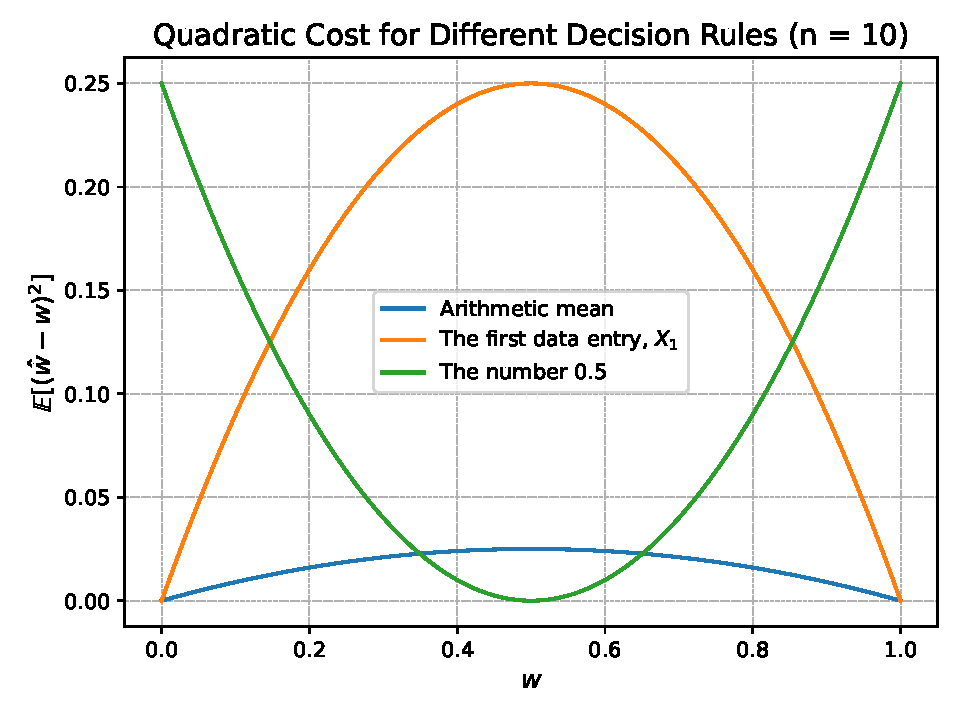
\includegraphics[width=1\textwidth]{figures/ber_example.pdf}
		\caption{The quadratic cost, $\mathbb{E}[(\hat{w} - w)^2]$, for three different decision rules: the arithmetic mean (blue), the first data entry $X_1$ (orange), and the constant value $0.5$ (green).}
		\label{fig:pen}
	\end{figure}
	
\end{example}

\begin{example}
	\emph{Determine the maximum likelihood estimate of $w$ for the model\newline $(\{0,1\},\{Ber(w)\}_{w\in(0,1)})$.}\newline
	
	\noindent In this case
	\begin{equation}
		\begin{split}
			p(D_s|D_x,w,I)=\prod_{i=1}^nw^{x_i}(1-w)^{1-x_i}.
		\end{split}
	\end{equation}
	Let $l(w)\equiv ln p(D_s|D_x,w,I)$, then
	\begin{equation}
		\begin{split}
			\argmax_wl(w) & = \argmax_wp(D_s|D_x,w,I)\\
			&= \argmax_w\ln \bigg(\prod_{i=1}^nw^{x_i}(1-w)^{1-x_i}\bigg)\\
			&=\argmax_w \bigg[\ln w\sum_{i=1}^nx_i + \ln(1-w)\sum_{i=1}^n(1-x_i)\bigg]
		\end{split}
	\end{equation}
	Now 
	\begin{equation}
		\frac{d}{dw}l(w)=\frac{\sum_{i=1}^nx_i}{w}-\frac{n-\sum_{i=1}^nx_i}{1-w}
	\end{equation}
	Requiring the derivative to vanish means the maximum likelihood estimate of $w$ is given by
	\begin{equation}
		\hat{w}_{\text{MLE}}=\frac{1}{n}\sum_{i=1}^nx_i.
	\end{equation}
\end{example}
\begin{example}
	\emph{Determine the maximum likelihood estimate of $w$ for the model\newline $([0,\infty),\{\text{Exp}(w)\}_{w>0})$.}\newline
	
	\noindent In this case
	\begin{equation}
		\begin{split}
			p(D_s|D_x,w,I)=\prod_{i=1}^nw e^{-w x_i}.
		\end{split}
	\end{equation}
	Let $l(w)\equiv ln p(D_s|D_x,w,I)$, then
	\begin{equation}
		\frac{d}{dw}l(w)=\frac{n}{w}-\sum_{i=1}^nx_i
	\end{equation}
	Requiring the derivative to vanish means the maximum likelihood estimate of $w$ is given by
	\begin{equation}
		\hat{w}_{\text{MLE}}=\frac{1}{\frac{1}{n}\sum_{i=1}^nx_i}.
	\end{equation}
\end{example}








	
	\cleardoublepage % Empty page before the start of the next part
	
	\part{Bayesian Statistics} % First part of the thesis
	\label{part:bayesian}
	
	% CHP: Introduction to Bayesian statistics
	\chapter{Bayesian Statistics Introduction}
Bayesian statistics is based on \dfref{def:bayesian_statistics}, which follows the definition of subjective probability (\dfref{def:subjective_probability}) and the treating the parameters as realizations of a random variable (\axref{ax:parameter_variable}). The Bayesian framework originally come from the work of \citet{Bayes:63} and \citet{laplace_thorie_1812} with much of the modern discussions and formalism created later by \citet{Finetti1937LaP,Jeffreys1940} and \citet{Savage1954}.\newline
In the Bayesian paradigm, it is assumed that Natures decisions can be captured by a statistical model with parameters that are modeled as realizations of random variables. This means that the probability $p(S=s|X=x,D,I)$ in equation \EQref{eq:decision_rule3} depend on the parameters $w_1,\dots w_n$ of the statistical model. Introducing the shorthand notation $W=w_1\dots W=w_n \rightarrow w$, $dw_1\dots dw_n \rightarrow dw$ and $X=x \rightarrow x$, then
\begin{equation}
	\begin{split}
		p(s|x,D,I) &= \int dw p(w,s|x,D,I)\\
		& = \int dw p(s|w,x,D,I)p(w|x,D,I)
	\end{split}
	\label{eq:hest1}
\end{equation}
\begin{example}
	Writing out the shorthand notation
	\begin{equation}
		\begin{split}
			p(W=w_1,\dots,W= w_n,S = s|X = x,D,I)&\rightarrow p(w,s|x,D,I),\\
			dw_1\dots dw_n &\rightarrow dw.\\
		\end{split}
	\end{equation}
\end{example}

To evaluate $p(w|D,I)$ a combination of the chain rule (\thref{theorem:chain_rule}), Bayes' theorem (\thref{theorem:bayes_theorem}) and marginalization (\thref{theorem:law_of_total_probability}) can be employed viz
\begin{equation}
	\begin{split}
		p(w|x,D,I) &= p(w|D,I)\\
		&= \frac{p(D_s|w,D_x,I)p(w|I)}{p(D_s|D_x,I)},
	\end{split}
	\label{eq:pa2}
\end{equation}
where $D_s= \{S=s_1\dots S=s_n\}$, $D_x = \{X=x_1,\dots X=x_n\}$ and $p(D_s|D_x,I)$ can be expanded via marginalization and \axref{ax:observation_relevance} has been used for the first and second equality.

\begin{axiom}[Relevance of Observations]
	\label{ax:observation_relevance}
	The Robot's observations are relevant for estimating Nature's model only when they map to known actions of Nature.
\end{axiom}

$p(w|I)$ is the Robot's prior belief about $w$. $p(D_s|w,D_x,I)$ is the likelihood of the past observations of Nature's actions, and $p(w|D,I)$ called the posterior distribution represent the belief of the Robot after seeing data. The prior distribution depends on parameters that must be specified and cannot be learned from data since it reflects the Robot's belief before observing data. These parameters are included in the background information, $I$. From \EQref{eq:pa2}, it is evident that, given the relevant probability distributions are specified, the probability of a parameter taking a specific value follows deductively from probability theory. The subjectivity arises from the assignment and specification of probability distributions which depend on the background information. 
	
	% CHP: Assigning a cost function
	\chapter{Regression}
\label{chp:regression}
Regression involves the Robot building a model, $f: \Omega_W\times \Omega_X\mapsto\mathbb{R}$, with associated parameters $w\in \Omega_W$, that estimates Nature's actions $S$ based on observed data $X$. Note that the output of $f$ is $\mathbb{R}$ implying that $S$ is assumed continuos. The model $f$ acts as a proxy for the Robot in that it on behalf of the Robot estimates the action of Nature given an input. Hence, in providing an estimate, the model must make a choice, similar to the Robot and thus the Robot must pick a cost function for the model. In this study, the quadratic cost function from \dfref{def:quadratic_cost} will be considered to review the subject. From \thref{theorem:expectation_decision_rule} the best action for the Robot can be written
\begin{equation}
	U^*(x) = \int ds s p(s|x,D,I)
	\label{eq:q1}
\end{equation}
Assuming the actions of Nature follow a normal distribution with the function $f$ as mean and an unknown variance, $\xi\in \Omega_W$
\begin{equation}
	p(s|x,w,\xi,I)=\sqrt{\frac{\xi}{2\pi}} e^{-\frac{\xi}{2}(f(w,x)-s)^2}.
	\label{f_dist}
\end{equation}
Using \EQref{f_dist} and marginalizing over $\xi,w$
\begin{equation}
	\begin{split}
		p(s|x,D,I) &= \int p(s,w,\xi|x,D,I) dw d\xi\\
		& = \int p(s|x,w,\xi,D,I)  p(w,\xi|x,D,I)dw d\xi\\
		& = \int p(s|x,w,\xi,I)  p(w,\xi|D,I)dw d\xi,\\
	\end{split}
	\label{eq:q2}
\end{equation}
where it has been used that $p(s|w,\xi,x,D,I) = p(s|w,\xi,x,I)$ since by definition $f$ produce a $1-1$ map of the input $x$ (\EQref{f_dist}) and $p(w,\xi|x,D,I) = p(w,\xi|D,I)$ from \axref{ax:observation_relevance}. Using \EQref{eq:q2} in \EQref{eq:q1}\footnote{Note that a function of a random variable is itself a random variable, so $f$ is a random variable.}
\begin{equation}
	\begin{split}
		U^*(x) & = \int f(w,x)  p(w,\xi|D,I) dw d\xi,\\
		& = \mathbb{E}[f|x,D,I]
	\end{split}
	\label{eq:q3}
\end{equation}	
where it has been used that
\begin{equation}
	\begin{split}
		\mathbb{E}[S|x,w,\xi,I] &= \int s p(s|x,w,\xi,I) dy\\
		&= f(w,x)
	\end{split}
\end{equation}
according to \EQref{f_dist}. Using Bayes theorem (\thref{theorem:bayes_theorem})
\begin{equation}
	p(w,\xi|D,I) = \frac{p(D_s|D_x,w,\xi,I)p(w,\xi|D_x,I)}{p(D_s|D_x,I)}
	\label{eq:bayes2}
\end{equation}
where from marginalization (\thref{theorem:law_of_total_probability})
\begin{equation}
	p(D_s|D_x,I) = \int p(D_s|D_x,w,\xi,I)p(w,\xi|D_x,I) dw d\xi.
\end{equation}
Assuming the past actions of Nature are independent and identically distributed, the likelihood can be written (using equation \EQref{f_dist})
\begin{equation}
	p(D_s|D_x,w,\xi,I) = \bigg(\frac{\xi}{2\pi}\bigg)^\frac{n}{2}\prod_{i=1}^n e^{-\frac{\xi}{2}(f(w,x_i)-s_i)^2}
	\label{reg:likelihood}
\end{equation}
From the chain rule (see \thref{theorem:chain_rule}) and \thref{ax:observation_relevance}
\begin{equation}
		p(w,\xi|D_x,I) = p(w|\xi,I)p(\xi|I).
\end{equation}
Assuming the distributions of the $w$'s are i) independent of $\xi$ and ii) normally distributed\footnote{The normally distributed prior is closely related to weight decay~\citep{Plaut1986}, a principle conventionally used in frequentist statistics to avoid the issue of overfitting.} with zero mean and a precision described by a hyperparameter, $\lambda$. 	 
\begin{equation}
	\begin{split}
		p(w|\xi,I) & = p(w|I)\\
		& = \int p(w|\lambda,I)p(\lambda|I)d\lambda
	\end{split}
	\label{eq:prior1}
\end{equation}
The precision is constructed as a wide gamma distribution\index{Gamma distribution} so as to approximate an objective prior
\begin{equation}
	p(w|\lambda,I)p(\lambda|I)
	= \prod_{q=1}^{\tilde{n}} \frac{\lambda_q^\frac{n_q}{2}}{(2\pi)^\frac{n_q}{2}}e^{-\frac{\lambda_q}{2}\sum_{l=1}^{n_q}w_l^2}\frac{\beta_q^{\alpha_q}}{\Gamma(\alpha_q)}\lambda_q^{\alpha_q-1}e^{-\beta_q \lambda_q}
	\label{eq:prior}
\end{equation}
where $\alpha_q,\beta_q$ are prior parameters (a part of the background information) and $\tilde{n}$ is the number of hyper parameters. In the completely general case $\tilde{n}$ would equal the number of parameters $w$, such that each parameter has an independent precision. In practice, the Robot may consider assigning some parameters the same precision, e.g. for parameters in the same layer in a neural network. Since $p(\xi|I)$ is analogous to $p(\lambda|I)$ -- in that both are prior distributions for precision parameters -- $p(\xi|I)$ is assumed to be a wide gamma distribution, then
\begin{equation}
	\begin{split}
		p(\xi|I) & = \text{Ga}(\xi|\tilde{\alpha},\tilde{\beta})\\
		& =\frac{\tilde{\beta}^{\tilde{\alpha}}}{\Gamma(\tilde{\alpha})}\xi^{\tilde{\alpha}-1}e^{-\tilde{\beta} \xi}.
	\end{split}
	\label{p7}
\end{equation}
At this point equation \EQref{eq:q1} is fully specified (the parameters $\alpha,\beta,\tilde{\alpha},\tilde{\beta}$ and the functional form of $f(w,x)$ are assumed specified as part of the background information) and can be approximated by obtaining samples from $p(w,\xi,\lambda|D,I)$ via HMC~\citep{Hammersley1964,Duane:1987de,Neal:1996,Neal2012} (see \appref{app:HMC} for a review of HMC). The centerpiece in the HMC algorithm is the Hamiltonian defined viz~\citep{Neal:1996,Neal2012}
\begin{equation}
	H \equiv  \sum_{q=1}^{\tilde{n}}\sum_{l=1}^{n_q}\frac{p_{l}^2}{2m_{l}}-\ln[p(w,\xi,\lambda|D,I)]+const,
	\label{eqh}
\end{equation}
where 
\begin{equation}
	p(w,\xi|D,I) = \int d\lambda p(w,\xi,\lambda|D,I).
	\label{eq:ss}
\end{equation}
Besides its function in the HMC algorithm, the Hamiltonian represent the details of the Bayesian model well and should be a familiar sight for people used to the more commonly applied frequentist formalism\index{Frequentist statistics} (since, in this case, it is in form similar to a cost function comprised of a sum of squared errors, weight decay on the coefficients and further penalty terms~\citep{hastie_09,murphy2013machine,Goodfellow2016}). Using \EQref{eq:bayes2}-\EQref{eq:ss} yields
\begin{equation}
	\begin{split}
		H&=\sum_{q=1}^{\tilde{n}}\sum_{l=1}^{n_q}\frac{p_{l}^2}{2m_{l}}+\frac{n}{2}[\ln(2\pi)-\ln(\xi)] +\frac{\xi}{2}\sum_{i=1}^{n}(f(w,x_i)-s_i)^2\\
		&\quad+\sum_{q=1}^{\tilde{n}}\bigg(\ln(\Gamma(\alpha_q))-\alpha_q\ln(\beta_q)+(1-\alpha_q)\ln(\lambda_q)+\beta_q\lambda_q\\
		&\qquad\qquad+\frac{n_q}{2}(\ln(2\pi)-\ln(\lambda_q))+\frac{\lambda_q}{2}\sum_{l=1}^{n_q}w_l^2\bigg)\\
		&\quad+\ln(\Gamma(\tilde{\alpha}))-\tilde{\alpha}\ln(\tilde{\beta})+(1-\tilde{\alpha})\ln(\xi)+\tilde{\beta}\xi+const.
	\end{split}
	\label{eqh2}
\end{equation}

	\begin{example}
	\index{Example: HMC Hamiltonian variable change}
	Let $\xi \equiv e^\zeta$, such that $\zeta\in [-\infty,\infty]$ maps to $\xi\in[0,\infty]$ and $\xi$ is ensured to be positive definite regardless of the value of $\zeta$. Using the differential $d\xi =  \xi d\zeta$ in \EQref{eq:q3} means $p(\theta,\xi,\lambda|D,I)$ is multiplied with $\xi$. Hence, when taking $-\ln(p(\theta,\xi,\lambda|D,I))$ according to \EQref{eqh}, a $-\ln(\xi)$ is added to the Hamiltonian. In practice this means
	\begin{equation}
		(1-\tilde{\alpha})\ln(\xi)\in H\Rightarrow -\tilde{\alpha}\ln(\xi).
	\end{equation} 	
\end{example}



\begin{example}
	Suppose there is a game between a Robot and Nature in which the Robot objective is to guess the position of the Robot. The Robot is given measurements of its velocity and acceleration, at any time step and must formulate a belief about its position. Nature decides the true position of the Robot and will penalize the Robot according to the deviation between the Robots estimate of its position and the true position viz (\dfref{def:quadratic_cost})
	\begin{equation}
		C(U(x),s) = (U(x)-s)^2,
	\end{equation}
	where $s$ is the true position $U(x)$ is the Robots estimate based on data $x$ containing velocity and acceleration measurements. 
	\begin{figure}[H]
		\centering
		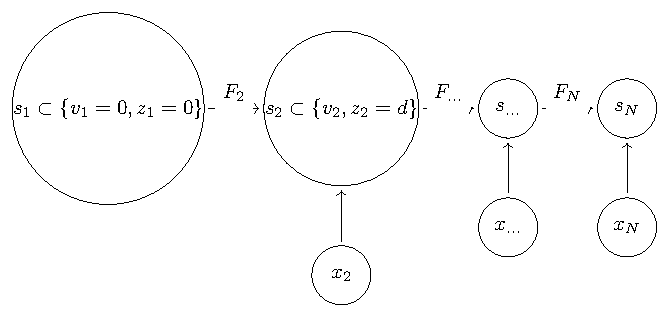
\includegraphics[width = 0.8\textwidth]{figures/graph.pdf}
		\caption{}
		\label{fig:1}
	\end{figure}
	Suppose the Robot is given all historical data, then the expected cost can be written
	\begin{equation}
		\mathbb{E}_{S|X}[C(U(X),S|s_1,\{x\}_{2:N},I)] = \int ds (U(x_N)-s)^2p(s|s_1,\{x\}_{2:N},I).
	\end{equation}
	The optimal decision is defined by
	\begin{equation}
		\frac{d}{dU(X)}\bigg(\mathbb{E}_{S|X}[C(U(X),S|s_1,\{x\}_{2:N},I)]\bigg)\bigg|_{U(x_N)=U^*(x_N)} = 0
	\end{equation}
	leading to (\thref{theorem:expectation_decision_rule})
	\begin{equation}
		U^*(x_N) = \mathbb{E}[S_{N}|s_1,\{x\}_{2:N},I].
		\label{eq:dr}
	\end{equation}
	The inutitive interpretation of \EQref{eq:dr} is that the optimal decision of the Robot is to estimate the position that it expects Nature to have chosen. Now
	\begin{equation}
		\mathbb{E}[S_{N}|s_1,\{x\}_{2:N},I] = \int ds_{N} s_N p(s_N|s_1,\{x\}_{2:N},I).
		\label{eq:a5}
	\end{equation}
	Assume that
	\begin{equation}
		\begin{split}
			p(s_i|s_{i-1},I) &= N(s_i|\mu_i = F_is_{i-1}+b_i,\Sigma_i = Q_i),\\
			p(x_i|s_{i},I) &= N(x_i|\mu_i = H_is_{i}+d_i,\Sigma_i = R_i)
		\end{split}
		\label{eq:a2}
	\end{equation}
	Hence, $p(s_N|s_1,\{x\}_{2:N},I)$ must be reformulated such that the above can be utilized. 
	Now
	\begin{equation}
		\begin{split}
			p(s_N|s_1,\{x\}_{2:N},I) &= \frac{p(x_{N}|s_N,s_1,\{x\}_{2:N-1},I)p(s_N|s_1,\{x\}_{2:N-1},I)}{p(x_{N}|s_1,\{x\}_{2:N-1},I)}\\
			&= \frac{p(x_{N}|s_N,I)p(s_N|s_1,\{x\}_{2:N-1},I)}{p(x_{N}|s_1,\{x\}_{2:N-1},I)}\\
		\end{split}
		\label{eq:a3}
	\end{equation}
	where
	\begin{equation}
		\begin{split}
			p(s_N|s_1,\{x\}_{2:N-1},I) &= \int ds_{N-1}p(s_N,s_{N-1}|s_1,\{x\}_{2:N-1},I)\\
			&= \int ds_{N-1}p(s_N|s_{N-1})p(s_{N-1}|s_1,\{x\}_{2:N-1},I)\\
			&=N(s_{N}|\mu_{N|N-1},\Sigma_{N|N-1})
		\end{split}
		\label{eq:a1}
	\end{equation}
	where 
	\begin{equation}
		\begin{split}
			\mu_{N|N-1} &= F_{N}\mu_{N-1}+b_N\\
			\Sigma_{N|N-1} &= F_{N}\Sigma_{N-1}F_{N}^T+Q_{N}\\
		\end{split}
	\end{equation}
	Using \EQref{eq:a1} and \EQref{eq:a2} in \EQref{eq:a3} then yields~\citep{murphy2023probabilistic}
	\begin{equation}
		p(s_N|s_1,\{x\}_{2:N},I) = N(s_N|\mu_{N},\Sigma_N)
		\label{eq:a4}
	\end{equation}
	where
	\begin{equation}
		\begin{split}
			\mu_{N} &= \mu_{N|N-1}+K_N(x_N-\hat{x}_N),\\
			\Sigma_{N} &= \Sigma_{N|N-1}-K_NS_NK_N^T,\\
			K_N & = \Sigma_{N|N-1}H_N^TS_N^{-1},\\
			\hat{x}_N&= H_N\mu_{N|N-1}+d_N,\\
			S_N & = H_N\Sigma_{N|N-1}H_N^T+R_N\\
		\end{split}
	\end{equation}
	Combining \EQref{eq:a4} with \EQref{eq:a5} then yields the optimal decision for the Robot
	\begin{equation}
		\mathbb{E}[S_{N}|s_1,\{x\}_{2:N},I] = \mu_{N}.
	\end{equation}
	
\end{example}

\begin{example}
	Consider a Robot moving in one dimension. Every time interval $\Delta t$, the Robot will sample a wheel counter and an accelerometer. The wheel counter will be incremented every distance $d$. The Robot is interested in knowing its position and velocity. Expand the position viz
	\begin{equation}
		z(t+\Delta t)=z(t)+\Delta t \frac{dz(t)}{dt}+\frac{1}{2}(\Delta t)^2\frac{d^2z(t)}{dt^2}+\mathcal{O}(\Delta t^3)
	\end{equation}
	which discretize to
	\begin{equation}
		z_k\simeq z_{k-1}+\Delta t v_{k-1}+\frac{1}{2}(\Delta t)^2a_{k-1},
	\end{equation}
	where $\Delta t = \text{const}$ and
	\begin{equation}
		\begin{split}
			v_k &\simeq v_{k-1}+\Delta t a_{k-1},\\
			a_k &\simeq a_{k-1},
		\end{split}
	\end{equation}
	This means
	\begin{equation}
		\begin{split}
			s_k &= \begin{pmatrix}
				z_k\\ v_{k} \\ a_k\\
			\end{pmatrix}\\
			& \simeq \underbrace{\begin{pmatrix}
					1 & \Delta t & \frac{1}{2}\Delta t^2  \\
					0 & 1 & \Delta t  \\
					0 & 0 & 1  \\
			\end{pmatrix}}_{=F_k}\begin{pmatrix}
				z_{k-1}\\ v_{k-1} \\ a_{k-1}\\
			\end{pmatrix}
		\end{split}
	\end{equation}
	where $b_k=\emptyset$ for simplicity. Now take
	\begin{equation}
		\begin{split}
			x_k &= \begin{pmatrix}
				c_k \\ a_k
			\end{pmatrix}\\
			&= \underbrace{\begin{pmatrix}
					d^{-1} & 0 & 0\\
					0 & 0 & 1 
			\end{pmatrix}}_{=H_k}\begin{pmatrix}
				z_{k-1}\\ v_{k-1} \\ a_{k-1}\\
			\end{pmatrix}+r_k
		\end{split}
	\end{equation}
	where $r_k \sim N(0,R_k)$ with 
	\begin{equation}
		R_k = \begin{pmatrix}
			\sigma_z^2 & \sigma_z\sigma_a\\
			\sigma_z\sigma_a & \sigma_a^2 \\
		\end{pmatrix},
	\end{equation}
	where $\sigma_z$ and $\sigma_a$ are estimated from observations. The process noise can be determined viz~\href{https://github.com/rlabbe/Kalman-and-Bayesian-Filters-in-Python/blob/master/07-Kalman-Filter-Math.ipynb}{Kalman link}
	\begin{equation}
		Q_k = \begin{pmatrix}
			\frac{\Delta t^4}{4} & \frac{\Delta t^3}{2} & \frac{\Delta t^2}{2}\\
			\frac{\Delta t^3}{2} & \Delta t^2 & \Delta t\\
			\frac{\Delta t^2}{2} & \Delta t & 1\\
		\end{pmatrix}\sigma^2,
	\end{equation}
	where $\sigma \sim \Delta a$.
\end{example}

	\chapter{Classification}
\label{chp:baycl}
Classification is the discrete version of regression, meaning it involves the Robot building a model, $f: \Omega_W\times \Omega_X\mapsto[0,1]$, with associated parameters $w\in \Omega_W$, that estimates Nature's actions $S$ based on observed data $X$. As opposed to regression, the random variable $S$ is now discrete and the function is identified with the probability of each action
\begin{equation}
	p(S = s|x,w,I)= f_{S = s}(w,x),
	\label{f_dist2}
\end{equation}
with
\begin{equation}
	\sum_{s\in\mathbb{S}} p(S = s|x,w,I) = 1.
\end{equation}
In this case, the Robot's action space is equal to Natures action space, with the possible addition of a reject option, $\Omega_U=\Omega_S\cup \text{"Reject"}$. To reivew this subject the Robot will be considered to be penalized equally in case of a classification error, which corresponds to the $0-1$ cost function, with the addition of a reject option at cost $\lambda$. This means
\begin{equation}
	C(U(x),s) = 1- \delta_{U(x),s}+(\lambda-1)\delta_{U(x),\text{"Reject"}}.
\end{equation}
The optimal decision rule for the robot can the be written
\begin{equation}
	\begin{split}
		U^*(x) & = \arg\min_{U(x)}\mathbb{E}[C(U(X), S)|x,D,I]\\
		&= \arg\min_{U(x)}\bigg(\sum_{s}C(U(x),s)p(S = s|x,D,I)\\
		&\qquad\qquad\qquad+(\lambda-1)\delta_{U(x),\text{"Reject"}}\bigg)\\
		& = \arg\min_{U(x)}\bigg(1- p(S=U(x)|x,D,I)\\
		&\qquad\qquad\qquad+(\lambda-1)\delta_{U(x),\text{"Reject"}}\bigg).
	\end{split}
	\label{eq:expected_cost1}
\end{equation}
In absence of the reject option, the optimal decision rule is to pick the MAP, similar to \thref{theorem:MAP}. Using \EQref{f_dist2} and marginalizing over $w$
\begin{equation}
	\begin{split}
		p(S= U(x)|x,D,I) &= \int p(S = U(x),w|x,D,I) dw \\
		& = \int p(S = U(x)|x,w,D,I)  p(w|x,D,I)dw \\
		& = \int p(S = U(x)|x,w,I)  p(w|D,I)dw \\
		& = \int f_{S = U(x)}(w,x)  p(w|D,I)dw \\
		& = \mathbb{E}[f_{S = U(x)}(w,x)|D,I],\\
	\end{split}
	\label{eq:q5}
\end{equation}
where for the second to last equality it has been assumed that $p(S = U(x)|w,x,D,I) = p(S = U(x)|w,x,I)$ since by definition $f$ (see \EQref{f_dist2}) produce a $1-1$ map of the input $x$ and $p(w|x,D,I) = p(w|D,I)$ from \axref{ax:observation_relevance}. From Bayes theorem
\begin{equation}
	p(w|D,I) =\frac{p(D_s|D_x,w,I)p(w|D_x,I)}{p(D_s|D_x,I)},
\end{equation}
where from \axref{ax:observation_relevance} $p(w|D_x,I) = p(w|I)$. Assuming the distribution over $w$ is normally distributed with zero mean and a precision described by a hyperparameter, $\lambda$, 
\begin{equation}
	p(w|I) = \int p(w|\lambda,I)p(\lambda|I)d\lambda.
\end{equation}
where $p(w|\lambda,I)p(\lambda|I)$ is given by \EQref{eq:prior}. Assuming the past actions of Nature are independent and identically distributed, the likelihood can be written~\citep{Fischer1999} 
\begin{equation}
	\begin{split}
		p(D_s|D_x,w,I) &=\prod_{i=1}^{n}p(S = s_i|X = x_i,w,I)\\
		&=\prod_{i=1}^{n}f_{s_i}(w,x_i)\\
	\end{split}.
	\label{lik}
\end{equation}
At this point \EQref{eq:expected_cost1} is fully specified and can be approximated by HMC similarly to the regression case. In this case, the model can be represented by the Hamiltonian 
\begin{equation}
	H \equiv  \sum_{q}\sum_{l}\frac{p_{l}^2}{2m_{l}}-\ln(p(w,\lambda|D,I))+const
	\label{ham3}
\end{equation}
where
\begin{equation}
	p(w|D,I) = \int d\lambda p(w,\lambda|D,I).
\end{equation}
Using \EQref{eq:q5}-\EQref{lik} in equation \eqref{ham3} yields the Hamiltonian
\begin{equation}
	\begin{split}
		H&=\sum_{q=1}^{\tilde{n}}\sum_{l=1}^{n_q}\frac{p_{l}^2}{2m_{l}}-\sum_{i=1}^{n}\ln(f_{s_i}(w,x_i))+\text{const}\\
		&\quad+\sum_{q=1}^{\tilde{n}}\bigg(\ln(\Gamma(\alpha_q))-\alpha_q\ln(\beta_q)+(1-\alpha_q)\ln(\lambda_q)+\beta_q\lambda_q\\
		&\qquad \qquad+\frac{n_q}{2}(\ln(2\pi)-\ln(\lambda_q))+\frac{\lambda_q}{2}\sum_{l=1}^{n_q}w_l^2\bigg)\\
	\end{split}.
	\label{ham2}
\end{equation}
Sampling \EQref{ham2} yields a set of coefficients which can be used to compute $\mathbb{E}[f_s(w,x)|D,I]$ which in turn (see \EQref{eq:q5}) can be used to compute $U^*(x)$.
	\begin{example}
	\index{Example: Bayesian decision theory}
	\emph{Consider a discrete action space with an observation $X=x$ and available data $D$. Picking a class corresponds to an action, so classification can be viewed as a game against nature, where nature has picked the true class and the robot has to pick a class as well. Suppose there are only two classes and the cost function is defined by the matrix}
	\begin{center}
		\begin{tabular}{ c  c  c  c }
			&& $S$& \\
			&& $s_1$ & $s_2$  \\
			\cline{3-4}
			$U(x)$ & $u_1$& \multicolumn{1}{|l}{$0$} &\multicolumn{1}{l|}{$\lambda_{01}$}  \\
			& $u_2$& \multicolumn{1}{|l}{$\lambda_{10}$} & \multicolumn{1}{l|}{0} \\
			\cline{3-4}
		\end{tabular}
	\end{center}
	\begin{enumerate}
		\item \emph{Show that the decision $u$ that minimizes the expected loss is equivalent to setting a probability threshold $w$ and predicting $U(x)=u_1$ if $p(S=s_1|x,D,I) < w$ and $U(x)=u_2$ if $p(S=s_2|x,D,I)\geq w$. What is $w$ as a function of $\lambda_{01}$ and $\lambda_{10}$?}\newline
		
		The conditional expected cost
		\begin{equation}
			\begin{split}
				\mathbb{E}_{S|X}[C(u, S)|x,D,I] & = \sum_sC(u,S=s)p(S=s|x,D,I)\\
				& = C(u,S=s_1)p(S=s_1|x,D,I)\\
				& \quad+C(u,S=s_2)p(S=s_2|x,D,I)\\
			\end{split}
		\end{equation}
		For the different possible actions
		\begin{equation}
			\begin{split}
				\mathbb{E}_{S|X}[C(u_1, S)|x,D,I] &= \lambda_{01}p(S=s_2|x,D,I),\\
				\mathbb{E}_{S|X}[C(u_2, S)|x,D,I] &= \lambda_{10}p(S=s_1|x,D,I),\\
			\end{split}
		\end{equation}
		$U(x)=u_1$ iff
		\begin{equation}
			\mathbb{E}_{S|X}[C(u_1,S)|x,D,I]<\mathbb{E}_{S|X}[C(u_1,S)|x,D,I])
		\end{equation}
		meaning
		\begin{equation}
			\begin{split}
				\lambda_{01}p(S=s_2|x,D,I)&<\lambda_{10}p(S = s_1|x,D,I)\\
				&=\lambda_{10}(1-p(S =s_2|x,D,I))
			\end{split}
		\end{equation}
		meaning $U(x) = u_0$ iff
		\begin{equation}
			p(S=s_2|x,D,I)<\frac{\lambda_{10}}{\lambda_{01}+\lambda_{10}}=w
		\end{equation}
		
		
		\item \emph{Show a loss matrix where the threshold is $0.1$.}\newline
		
		$w = \frac{1}{10}=\frac{\lambda_{10}}{\lambda_{01}+\lambda_{10}} \Rightarrow \lambda_{01}=9\lambda_{10}$ yielding the loss matrix
		
		\begin{center}
			\begin{tabular}{ c  c  c  c }
				&& $S$& \\
				&& $s_1$ & $s_2$  \\
				\cline{3-4}
				$U(x)$ & $u_1$& \multicolumn{1}{|l}{$0$} &\multicolumn{1}{l|}{$9\lambda_{10}$}  \\
				& $u_2$& \multicolumn{1}{|l}{$\lambda_{10}$} & \multicolumn{1}{l|}{0} \\
				\cline{3-4}
			\end{tabular}
		\end{center}
		
		You may set $\lambda_{10}=1$ since only the relative magnitude is important in relation to making a decision.
		
	\end{enumerate}
	
	
\end{example}


\begin{example}
	\index{Example: Bayesian decision theory}
	\emph{In many classification problems one has the option of assigning $x$ to class $k\in K$ or, if the robot is too uncertain, choosing a reject option. If the cost for rejection is less than the cost of falsely classifying the object, it may be the optimal action. Define the cost function as follows}
	\begin{equation}
		C(u,s)=\begin{cases}
			0 & \text{if correct classification ($u=s$)}\\
			\lambda_r & \text{if reject option $u=$ reject}\\
			\lambda_s & \text{if wrong classification ($u\neq s$)}\\
		\end{cases}.
	\end{equation}
	
	\begin{enumerate}
		\item \emph{Show that the minimum cost is obtained if the robot decides on class $u$ if $p(S=u|x,D,I)\geq p(S\neq u|x,D,I)$ and if $p(S=u|x,D,I)\geq 1-\frac{\lambda_r}{\lambda_s}$.}\newline
		
		The conditional expected cost if the robot does not pick the reject option, meaning $u\in \mathbb{U}\setminus\text{reject}$
		\begin{equation}
			\begin{split}
				\mathbb{E}_{S|X}[C(u, S)|x,D,I] & = \sum_s C(u,S=s)p(S=s|x,D,I)\\
				&= \sum_{s\neq u}\lambda_sp(S=s|x,D,I)\\
				&= \lambda_s(1-p(S=u|x,D,I))
			\end{split}
			\label{eq:cost1}
		\end{equation}
		where for the second equality it has been used that the cost of a correct classification is $0$, so the case of $S=u$ does not enter the sum. For the third equality it has been used that summing over all but $S=u$ is equal to $1-p(S=u|x,D,I)$. The larger $p(S=u|x,D,I)$, the smaller loss (for $\lambda_s>0$), meaning the loss is minimized for the largest probability. The conditional expected loss if the robot picks the reject option
		\begin{equation}
			\begin{split}
				\mathbb{E}_{S|X}[C(\text{reject}, S)|x,D,I]&= \lambda_r\sum_sp(S=s|x,D,I)\\
				&=\lambda_r.
			\end{split}
			\label{eq:cost2}
		\end{equation}
		Equation \eqref{eq:cost1} show picking $\arg\max_{u\in \mathbb{U}\setminus \text{reject}} p(S=u|x,D,I)$ is the best option among classes $u\neq \text{reject}$. To be the best option overall, it also needs to have lower cost than the reject option. Using equations \eqref{eq:cost1} and \eqref{eq:cost2} yields
		\begin{equation}
			(1-p(S=u|x,D,I))\lambda_s< \lambda_r
		\end{equation}
		meaning
		\begin{equation}
			p(S=u|x,D,I)\geq 1-\frac{\lambda_r}{\lambda_s}.
		\end{equation}
		
		\item \emph{Describe qualitatively what happens as $\frac{\lambda_r}{\lambda_s}$ is increased from $0$ to $1$.}\newline
		
		$\frac{\lambda_r}{\lambda_s}=0$ means rejection is rated as a successful classification -- i.e. no cost associated -- and this become the best option (rejection that is) unless $p(y=j|x)=1$, corresponding to knowing the correct class with absolute certainty. In other words; in this limit rejection is best unless the robot is certain of the correct class. $\frac{\lambda_r}{\lambda_s}=1$ means rejection is rated a misclassification -- i.e. $\lambda_r=\lambda_s$ -- and thus and "automatic cost". Hence, in this case rejection is never chosen. In between the limits, an interpolation of interpretations apply.
	\end{enumerate}
\end{example}



\begin{example}
	\paragraph{Setup:} Consider a farmer who wishes to retire and therefore would like to sell their set of live animals. For simplicity, assume that animals make up a simple group and a given person can either be interested in purchasing an animal or not -- the simplfication consist of not differentiating between different animal types. In order to sell their animals, the farmer needs to contact people with a sale in mind. For simplicity, the contact will be assumed to be via a telephone call only. The farmer can call (or not) with the intent to sell an animal to the recepient of the call. The recepient of the call can (or not) be interesed in purchasing an animal (Natures decision). Let $\Omega_U$ denote the set of the farmers actions and $\Omega_S$ the set of Natures actions, then
	\begin{equation}
		\begin{split}
			\Omega_U &= \{u_1 = \text{call}, u_2 = \text{don't call}\},\\
			\Omega_S &= \{s_1 = \text{interested}, s_2 = \text{not interested}\}.
		\end{split}
	\end{equation}
	A nuisance for the contacted people is associated to the call which is represented by the abstract monetary loss, $\lambda\in \mathbb{R}^+$. The degree to which people are annoyed by a sales call is independent in general and the monetary loss represents the average animosity generated and the associated moneraty loss connected to a worsened reputation. Aside from the nuisance associated with a sales call, there is also a moneraty reward for a successfull sale, $\psi$.	If the farmer cannot sell his animals, he will have them terminated with no associated cost in order not to spend additional time or money on them. Given these assumptions, the cost function can be represented by the matrix
	\begin{center}
		\begin{tabular}{  c  c  c }
			& $s_1=$ Interested & $s_2=$ Not interested  \\
			\cline{2-3}
			 $u_1 =$ Call& \multicolumn{1}{|l}{$\lambda-\psi$} &\multicolumn{1}{l|}{$\lambda$}  \\
			 $u_2=$ Don't call& \multicolumn{1}{|l}{$0$} & \multicolumn{1}{l|}{0} \\
			\cline{2-3}
		\end{tabular}
	\end{center}
	The farmer has available to them observations $X=x$ that contain information regarding the decesion Nature is going to make, $S=s$. The farmer also have a collection of past observations and resulting decisions of Nature, i.e. $D= \{(X=x_1,S=s_1),(X=x_2,S=s_2),\dots (X=x_n,S=s_n)\}= D_s\times D_s$. 
	
	\paragraph{Optimal decision rule:} The optimal decision for the farmer to call the $i$'th person can then be written viz
	\begin{equation}
		U^*(x) = \arg\min_{U(x)} \mathbb{E}_{S|X}[C(U(x), S)|X=x,D,I],
	\end{equation}
	where
	\begin{equation}
		\mathbb{E}_{S|X}[C(U(x), S)|X=x,D,I] = \sum_{s\in \mathbb{S}} C(U(x),s) p(S=s|X=x,D,I).
	\end{equation}
	Writing out the conditional expectation
	\begin{equation}
		\begin{split}
			\mathbb{E}[C(u_1, S)] & = \sum_sC(u_1,s)p(s)\\
			& = C(u_1,s_1)p(s_1|x,D,I) + C(u_1,s_2)p(s_2|x,D,I)\\
			& = (\lambda-\psi)p(s_1|x,D,I) + \lambda_i p(s_2|x,D,I),\\
			\mathbb{E}[C(u_2, S)] & = \sum_sC(u_2,s)p(s|x,D,I)\\
			& = C(u_2,s_1)p(s_1|x,D,I) + C(u_2,s_2)p(s_2|x,D,I),\\
			&=0
		\end{split}
	\end{equation}
	where the notation has been compressed to fit the equations to the page. The optimal decision rule $U^*(x)$ can be implicitly specified as picking $u_1$ (call) iff $\mathbb{E}_{S|X}[C(u_1, S)|x,D,I]<\mathbb{E}_{S|X}[C(u_2, S)|x,D,I]$, corresponding to picking $u_1$ (call) iff
	\begin{equation}
		(\lambda-\psi)p(S= s_1|x,D,I) + \lambda p(S= s_2|x,D,I) <0
	\end{equation}
	Since $p(S= s_1|x,D,I) +p(S= s_2|x,D,I) = 1$
	\begin{equation}
		\frac{\lambda}{\psi} < p(S= s_1|x,D,I)
		\label{eq:decision_rule}
	\end{equation}
	meaning the farmer should call (action $u_1$) iff the probability for the recepient of the call to be interested in at least one animal is larger than the penalty of calling divided by the gain of calling. 
	
	\paragraph{The Probability:} \EQref{eq:decision_rule} implicitly specify the decision rule for the farmer. $\lambda,\psi$ is assumed specified, so only the probability $p(S= s_1|x,D,I)$ remain to be specified. Suppose now a model, $f: \Omega_W\times \Omega_X\mapsto[0,1]$, with associated parameters $w\in \Omega_W$, that estimates Nature's actions $S$ based on observed data $X$ is introduced. Using marginalization and assuming independence 
	\begin{equation}
		\begin{split}
			p(S= s|x,D,I) &= \int p(S= s,w|x,D,I) dw \\
			& = \int p(S= s|x,w,D,I)  p(w|x,D,I)dw \\
			& = \int p(S= s|x,w,I)  p(w|D,I)dw. \\
		\end{split}
		\label{eq:q5}
	\end{equation}
	Combining \EQref{eq:q5} and \EQref{f_dist2}
	\begin{equation}
		\begin{split}
			p(S= s|x,D,I) & = \int f_{S = s}(w,x)  p(w|D,I)dw \\
			& = \mathbb{E}[f_{S = s}(w,x)|D,I].\\
		\end{split}
	\end{equation}
	From Bayes theorem \index{Bayes theorem}
	\begin{equation}
		p(w|D,I) =\frac{p(D_s|D_x,w,I)p(w|D_x,I)}{p(D_s|D_x,I)},
	\end{equation}
	where $p(w|D_x,I) = p(w|I)$. Assuming the distribution over $w$ is normally distributed with zero mean and a precision described by a hyperparameter, $\lambda$, 
	\begin{equation}
		p(w|I) = \int p(w|\lambda,I)p(\lambda|I)d\lambda.
		\label{eq:lambda}
	\end{equation}
	The precision is constructed as a wide gamma distribution so as to approximate an objective prior
	\begin{equation}
		p(w|\lambda,I)p(\lambda|I)
		= \prod_{q=1}^{\tilde{n}} \frac{\lambda_q^\frac{n_q}{2}}{(2\pi)^\frac{n_q}{2}}e^{-\frac{\lambda_q}{2}\sum_{l=1}^{n_q}w_l^2}\frac{\beta_q^{\alpha_q}}{\Gamma(\alpha_q)}\lambda_q^{\alpha_q-1}e^{-\beta_q \lambda_q}
		\label{eq:prior}
	\end{equation}
	Assuming the past actions of Nature are independent and identically distributed, the likelihood can be written 
	\begin{equation}
		\begin{split}
			p(D_s|D_x,w,I) &=\prod_{i=1}^{n}p(S = s_i|X = x_i,w,I)\\
			&=\prod_{i=1}^{n}f_{s_i}(w,x_i)\\
		\end{split}.
		\label{lik}
	\end{equation}
	Aside from the specification of the model $f$, $p(S= s|x,D,I)$ is at this point fully specified and can be approximated by HMC similarly to the regression case. In this case, the model can be represented by the Hamiltonian 
	\begin{equation}
		H \equiv  \sum_{q}\sum_{l}\frac{p_{l}^2}{2m_{l}}-\ln(p(w,\lambda|D,I))+const
		\label{ham3}
	\end{equation}
	where
	\begin{equation}
		p(w|D,I) = \int d\lambda p(w,\lambda|D,I).
	\end{equation}
	Using \EQref{eq:q5}-\EQref{lik} in \EQref{ham3} yields the Hamiltonian
	\begin{equation}
		\begin{split}
			H&=\sum_{q=1}^{\tilde{n}}\sum_{l=1}^{n_q}\frac{p_{l}^2}{2m_{l}}-\sum_{i=1}^{n}\ln(f_{s_i}(w,x_i))+\text{const}\\
			&\quad+\sum_{q=1}^{\tilde{n}}\bigg(\ln(\Gamma(\alpha_q))-\alpha_q\ln(\beta_q)+(1-\alpha_q)\ln(\lambda_q)+\beta_q\lambda_q\\
			&\qquad \qquad+\frac{n_q}{2}(\ln(2\pi)-\ln(\lambda_q))+\frac{\lambda_q}{2}\sum_{l=1}^{n_q}w_l^2\bigg)\\
		\end{split}.
		\label{ham2}
	\end{equation}
	
	\paragraph{Simple model:} Let
	\begin{equation}
		f_{S = s}(w,x_i) = \frac{e^{b_s+\sum_{q}a_{sq}x_{iq}}}{\sum_{k\in \mathbb{S}}e^{b_k+\sum_{q}a_{kq}x_{iq}}},
		\label{eq:f1}
	\end{equation}
	where $w = \{b,a\}$.
	
	\paragraph{Manual HMC:}	The Hamiltonian is given by
	\begin{equation}
		\begin{split}
			H&=\sum_{q=1}^{2}\sum_{l=1}^{2}\frac{p_{ql}^2}{2m_{ql}}-\sum_{i=1}^{n}\ln(f_{s_i}(w,x_i))\\
			&\quad+\ln(\Gamma(\alpha_a))-\alpha_a\ln(\beta_a)+(1-\alpha_a)\ln(\lambda_a)+\beta_a\lambda_a\\
			&\qquad \qquad+\frac{1}{2}(\ln(2\pi)-\ln(\lambda_a))+\frac{\lambda_a}{2}\sum_{j,q}a_{jq}^2\\
			&\quad+\ln(\Gamma(\alpha_b))-\alpha_b\ln(\beta_b)+(1-\alpha_b)\ln(\lambda_b)+\beta_b\lambda_b\\
			&\qquad \qquad+\frac{1}{2}(\ln(2\pi)-\ln(\lambda_b))+\frac{\lambda_b}{2}\sum_{j}b_j^2\\
		\end{split}
	\end{equation}
	$\lambda_j$ is positive definite. In order to uphold this numerically, let $\lambda_j = e^{\tau_j}$. When making this transformation, the integration measure of \EQref{eq:lambda} has to be transformed as well. This proceeds viz
	\begin{equation}
		d\lambda_j = \lambda_jd\tau_j,
	\end{equation}
	meaning effectively $\lambda_j$ is multiplied on $p(w,\lambda|D,I)$ such that $H \rightarrow H-\ln(\lambda_j)$. This means
	\begin{equation}
		(1-\alpha_j)\ln(\lambda_j)\in H \Rightarrow -\alpha_j \ln(\lambda_j).
	\end{equation}
	Additionally, it is convenient to pick out the $s_i$ via a one-hot target vector such that
	\begin{equation}
		\begin{split}
			H&=\sum_{q=1}^{2}\sum_{l=1}^{2}\frac{p_{ql}^2}{2m_{ql}}-\sum_{j\in \mathbb{S}}\sum_{i=1}^{n}s_{ij}\ln(f_{j}(w,x_i))\\
			&\quad+\ln(\Gamma(\alpha_a))-\alpha_a\ln(\beta_a)-\alpha_a\tau_a+\beta_ae^{\tau_a}\\
			&\qquad \qquad+\frac{1}{2}(\ln(2\pi)-\tau_a)+\frac{e^{\tau_a}}{2}\sum_{j,q}a_{jq}^2\\
			&\quad+\ln(\Gamma(\alpha_b))-\alpha_b\ln(\beta_b)-\alpha_b\tau_b+\beta_be^{\tau_b}\\
			&\qquad \qquad+\frac{1}{2}(\ln(2\pi)-\tau_b)+\frac{e^{\tau_b}}{2}\sum_{j}b_j^2\\
		\end{split}
	\end{equation}
	
	The derivatives are needed for the HMC algorithm
	\begin{equation}
		\frac{\partial H}{\partial a_{ml}} = -\sum_{i,j}\frac{s_{ij}}{f_{ij}}\frac{\partial f_{ij}}{\partial a_{ml}}+e^{\tau_a}a_{ml},\\
	\end{equation}
	\begin{equation}
		\begin{split}
			\frac{\partial f_{ij}}{\partial a_{ml}} & = \frac{e^{b_j+\sum_{q_1}a_{jq_1}x_{iq_1}}}{\sum_{k\in \mathbb{S}}e^{b_k+\sum_{q_2}a_{kq_2}x_{iq_2}}}\sum_{q_3}\delta_{jm}\delta_{q_3l}x_{iq_3}\\
			&\qquad-\frac{e^{b_j+\sum_{q_4}a_{jq_4}x_{iq_4}}}{(\sum_{k\in \mathbb{S}}e^{b_k+\sum_{q_5}a_{kq_5}x_{iq_5}})^2}\sum_{k'\in \mathbb{S}}e^{b_{k'}+\sum_{q_6}a_{k'q_6}x_{iq_6}}\sum_{q_7}\delta_{k'm}\delta_{q_7l}x_{iq_7}\\
			& = f_{ij}\delta_{jm}x_{il}- f_{ij}f_{im}x_{il}
		\end{split}
	\end{equation}
	where it has been used that
	\begin{equation}
		\frac{\partial a_{jq_3}}{\partial a_{ml}} = \delta_{jm}\delta_{q_3l}
	\end{equation}
	
	\begin{equation}
		\begin{split}
			\frac{\partial H}{\partial a_{ml}} &= -\sum_{i,j}\frac{s_{ij}}{f_{ij}}(f_{ij}\delta_{jm}x_{il}- f_{ij}f_{im}x_{il})+e^{\tau_a}a_{ml}\\
			& = \sum_ix_{il}(f_{im}-s_{im})+e^{\tau_a}a_m\\
		\end{split}
	\end{equation}
	\begin{equation}
		\frac{\partial H}{\partial b_m} = \sum_i(f_{im}-s_{im})+e^{\tau_b}b_m.
	\end{equation}
	\begin{equation}
		\frac{\partial H}{\partial \tau_m} = -\alpha_m+\beta_me^{\tau_m}-\frac{1}{2}+\frac{e^{\tau_m}}{2}\sum_jm_j^2.
	\end{equation}
	
	The masses for the HMC algorithm can be set by approximating the second order derivatives as fixed. Let
	\begin{equation}
		\begin{split}
			\frac{\partial^2 H}{\partial a_{ml}^2} &= \sum_ix_{il}\frac{\partial f_{im}}{\partial a_{ml}}+e^{\tau_a}\\
			& =\sum_ix_{il}^2f_{im}( 1- f_{im})+e^{\tau_a}\\
		\end{split}
	\end{equation}
	then taking $x_{il}^2\sim 1, f_{im}\sim \frac{1}{2}$ and any parameter $\sim 0$, meaning $e^{\tau_a} \sim 1$ yield the mass approximation
	\begin{equation}
		\begin{split}
			m_{ml}^{(a)} &\sim \frac{\partial^2 H}{\partial a_{ml}^2}\bigg|_{\text{fixed approximation}}\\
			& \sim N\cdot 1^2\cdot \frac{1}{2}(1-\frac{1}{2})+1\\
			&=\frac{N}{4} +1,
		\end{split}
	\end{equation}
	where $N$ is the number of data samples in $D_x$. Similarly
	\begin{equation}
		\begin{split}
			\frac{\partial^2 H}{\partial b_m^2} &= \sum_i\frac{\partial f_{im}}{\partial a_{ml}}+e^{\tau_b}\\
			& =\sum_if_{im}( 1- f_{im})+e^{\tau_b},
		\end{split}
	\end{equation}
	meaning (since $x_{il}^2\sim 1$)
	\begin{equation}
		\begin{split}
			m_{ml}^{(a)} &\sim \frac{\partial^2 H}{\partial b_{m}^2}\bigg|_{\text{fixed approximation}}\\
			& m_{ml}^{(b)}.
		\end{split}
	\end{equation}
	The precision parameter
	\begin{equation}
		\frac{\partial^2 H}{\partial \tau_q^2} = \beta_qe^{\tau_q}+\frac{e^{\tau_q}}{2}\sum_jq_j^2.
	\end{equation}
	Take $\beta_q = 3$, then
	\begin{equation}
		\begin{split}
			m_{q}^{(\tau)} &\sim \frac{\partial^2 H}{\partial \tau_{q}^2}\bigg|_{\text{fixed approximation}}\\
			&\sim 3.
		\end{split}
	\end{equation}
	
	
	
	
	\paragraph{Data:} Take $x=(\text{area},\text{number of animals})^T$ and $s=$ 2d one-hot vector, with $\dim(D)=1000$. $D$ is split into two sets $D^{(\text{training})}$ and $D^{(\text{test})}$, with $\dim(D^{(\text{training})})=\gamma\dim(D)$ and $\dim(D^{(\text{test})})=(1-\gamma)\dim(D)$ and $\gamma=0.6$. $D^{(\text{training})}$ will be used to train the model and $D^{(\text{test})}$ to evaluate the quality of the trained model. The underlying truth of Nature (unbeknownst to the model) is that an animal will be purchased iff
	\begin{equation}
		\text{total area}- 3.2\cdot\text{number of animals}\geq 3.2.
		\label{eq:nature}
	\end{equation}
	
	\paragraph{Training:} Using $D^{(\text{training})}$ as input, the algorithms the algorithms are trained for $2000$ iterations. The first $500$ iterations are taken as burn in to be conservative. The coefficients, $w$, for iterations $[500,2000]$ are used to make a model prediction viz
	\begin{equation}
		p(S= s|x,D,I)=\frac{1}{1500}\sum_{i=500}^{2000}f(w_i,x)
	\end{equation}
	The accuracy of the modeled probabilities can be gauged by considering the case where $\psi=2\lambda$ such that the decision rule (\EQref{eq:decision_rule}) becomes
	\begin{equation}
		\frac{1}{2} < p(S= s_1|x,D,I),
		\label{eq:decision_rule2}
	\end{equation}
	and the classification is driven by the probabilities alone. 
	
	
	\paragraph{PyMC HMC Algorithm:} PyMC is a probabilistic programming library for Python that allows users to build Bayesian models with a Python API and fit them using Markov Chain Monte Carlo methods \href{https://www.pymc.io/welcome.html}{PyMC link}. Using this API it is possible to create, train and test a PyMC-equivalent of the model described in the previous sections. The general approach to building a model using PyMC consists of stating the data generating process, specifying a likelihood, and related prior distributions for any parameters involved. While modeling the data generating process and framing the statistical problem correctly are never completely trivial and require some effort from the user it is rather straight forward to perform the Markov Chain Monte Carlo sampling with PyMC. The user do not need to do any calculations related to the Hamiltonian Monte Carlo method nor do they need to specifically handle any integrals. In addition, there is a range of predefined probability distributions both discrete and continuous readily available in the library such as the Gamma (figure \ref{fig:gamma}) and Normal distribution used for modeling the priors.
	\begin{figure}[H]
		\centering
		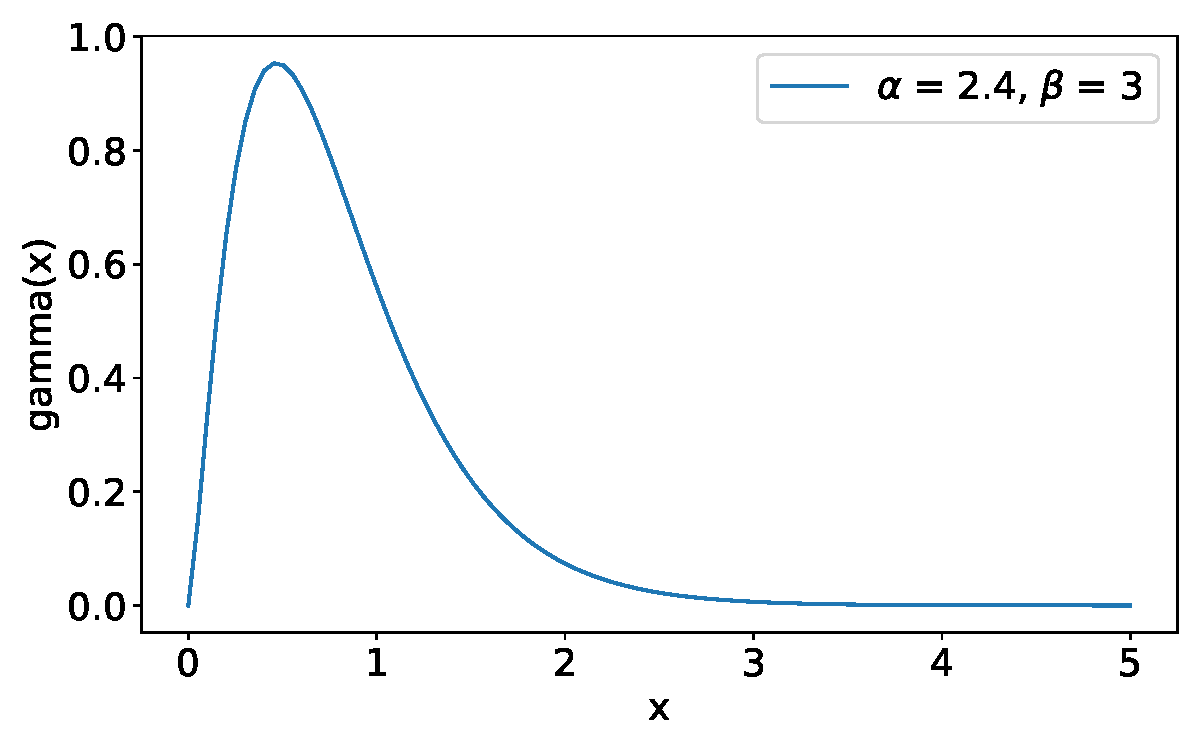
\includegraphics[width = 1\textwidth]{figures/gamma_dist.pdf}
		\caption{Plot of Gamma probability distribution used as priors for the precision parameters in Normal distributions.}
		\label{fig:gamma}
	\end{figure}
	The python code in \algref{algo:pymc_model} shows how the simple model can be declared using PyMC. All models in PyMC are declared using a "with pm.Model() as modelname"-statement, where pm is the abbreviated form of the PyMC package. Within this statement at range of random variables, data and their relations can be declared. The syntax for declaring a random variable by its probability distribution (such as pm.Normal) is to pass a name for the random variable as a string for the first argument. The rest of the arguments are typically values for the parameters specific to the distribution. PyMC random variables can often be used for stating parameters in other random variables forming a hierarchy of distributions as is the case for the precision variables used to model the variance for the normally distributed parameters a and b (see \EQref{eq:f1}) with zero mean. In the code example, these parameters are then combined deterministically with $D_x$ to constitute the data generating process of the simple model. $D_x$ is declared as a PyMC mutable object so that it will be possible later to change the values to generate predictions. As a last step the likelihood is declared. In PyMC this is the step where the relationship between the observed conditional ($D_s$) data and parameters is stated. As the output is the probabilities for the two classes a Multinomial distribution with the number of independent trials (n) equal to 1 is used as the likelihood. 
	
	\begin{algorithm}[H]
		\caption{PyMC Python Code}
		\begin{python}
			import pymc as pm
			import numpy as np
			with pm.Model() as classifier_model:
			covars = pm.MutableData('covars',data_x_training) 
			# Priors for precision
			precision_a = pm.Gamma('precision_a', alpha=2.4, beta=3)
			precision_b = pm.Gamma('precision_b', alpha=2.4, beta=3)
			# Priors for parameters
			param_a = pm.Normal('param_a', 
			0, 
			sigma=1/np.sqrt(precision_a),
			shape=(2,2))
			param_b = pm.Normal('param_b', 
			0, 
			sigma=1/np.sqrt(precision_b),
			shape=(2,))
			# Data generating process
			T = pm.Deterministic('T', pm.Math.exp(param_b + pm.math.dot(covars, param_a.T)))
			class_conditional_probability = pm.Deterministic('class_conditional_probability', T/T.sum(axis=1, keepdims=True))
			# Likelihood
			obs = pm.Multinomial('obs', n=1, p=class_conditional_probability, observed=data_s_training, shape=class_conditional_probability.shape)
		\end{python}
		\label{algo:pymc_model}
	\end{algorithm}
	
	
	After declaring the model it is possible to sample the posterior by calling the pm.sample() method. Burn-in can be controlled by setting the tune argument. The draw argument determines how many samples are being drawn while a number of chains can be run in parallel by setting the chains and cores (computational) arguments. 	
	\begin{algorithm}[H]
		\label{algo:posteriro}
		\caption{PyMC Posterior Python Code}
		\begin{python}
			with classifier_model:
			posterior = pm.sample(tune=512, draws=1024, chains=4, cores=4)
		\end{python}  
	\end{algorithm}
	
	Using the result of drawing samples from the distribution of model parameters (posterior) it is possible to draw from the posterior predictive distribution using the pm.sample\_posterior\_predictive() method. Without changing the input data this is equivalent to obtaining the result of applying the trained model on $D_x^{(\text{training})}$. By changing the input data to $D_x^{(\text{test})}$ using the pm.set\_data() method it is possible to obtain the posterior predictive distribution.
	
	\begin{algorithm}[H]
		\label{algo:posteriro_predictive}
		\caption{PyMC Posterior Python Code}
		\begin{python}
			with classifier_model:
			posterior_predictive = pm.sample_posterior_predictive(posterior)
			pm.set_data({'covars': data_x_test})
			posterior_predictive_test = pm.sample_posterior_predictive(posterior)
		\end{python}
	\end{algorithm}
	
	Using \EQref{eq:decision_rule2} for $D^{(\text{training})}$, the PyMC model correctly classify $598$ of $600$ data points. For $D^{(\text{test})}$, the model correctly classify $398$.
	
	\paragraph{Results: } The HMC algorithm have parameters "step\_scale" and "number\_of\_steps\_scale", which adjust the overall scale of the step lengths and number of steps in pase space. Ideally, the distance between points should be large, so that step scale should be small (what the step length is divided by should be small) and the number of steps should be large. Numerical stability only exist for step\_scale $\gtrsim 5$ (given accurate mass estimation) and thus only the number of steps remain as a variable to tune. In this study step\_scale $=10$ and number\_of\_steps\_scale $=1500$, where the latter is limited by reasonable computation time (to match approximately the pymc computation time). Given these parameters, the manual HMC algorithm misclassify a single training data point
	\begin{equation}
		x^{(\text{training})}_{\text{misclassified 1}} = \begin{pmatrix}
			3.21798365\\ 0\\
		\end{pmatrix}
		\label{eq:misclassified1_training}
	\end{equation}
	and two test data points
	\begin{equation}
		x^{(\text{test})}_{\text{misclassified 1}} = \begin{pmatrix}
			6.40501793\\ 1\\
		\end{pmatrix}, \quad x^{(\text{test})}_{\text{misclassified 2}} = \begin{pmatrix}
			9.60627827\\ 2\\
		\end{pmatrix}.
		\label{eq:misclassified1_test}
	\end{equation}
	With \EQref{eq:nature} in mind, it is clear that the misclassifications of \EQref{eq:misclassified1_training} and \EQref{eq:misclassified1_test} are close to the limit with respect to purchasing an animal.  
	
	
	The PyMC HMC Algorithm obtain misclassify two training data points; \EQref{eq:misclassified1_training} and 
	\begin{equation}
		x^{(\text{training})}_{\text{misclassified 2}} = \begin{pmatrix}
			12.80826256\\ 3\\
		\end{pmatrix}
		\label{eq:misclassified1_training2}
	\end{equation}
	and two test data points (\EQref{eq:misclassified1_test}).
	
	
	\paragraph{Summary and Discussion:} It has been shown how decision theory can be used in conjunction with statistics to make theoretically optimal decisions based on a user specified set of preferences (cost function). Using mock data, a "manual HMC algorithm" written by hand and a standard Python "PyMC HMC algorithm" have been compared. The two yield identical results on test data with the manual model yielding marginally better results on training data. Overall the performace is deemed equivalent both in terms of accuracy and computational speed. The manual HMC algorithm require the user to derive the gradients, write the sampling algorithm in Python and tune the algorith, whereas the latter only require a specification of the model via a standardized PyMC interface. Hence, from a user complexity perspective, the PyMC algorithm has a significant advantage.
\end{example}
	
	% CHP: Inference about Natures model
	\chapter{Making Inference About the Model of Nature}
In some instances, the robot is interested in inference related to the model of Nature. The observation $X=x$ by definition does not have an associated known action of Nature and thus by \axref{ax:observation_relevance} is disregarded in this context. From \EQref{eq:decision_rule3}
\begin{equation}
	U^*(D) = \arg\min_{U(D)} \mathbb{E}_{S|D}[C(U(D), S)|D,I]
	\label{eq:best_decision}
\end{equation}
where $S=s$ is interpreted as an action related to the model of Nature, e.g. Nature picking a given systematic that generates data.

\section{Selecting the Robot's Model}
\label{sec:model_selection}
Suppose the Robot must choose between two competing models, aiming to select the one that best represents Nature's true model. The two competing models could e.g. be two different functions $f$ in regression or two different probability distribution assignments. In this case the Robot has actions $u_1$ and $u_2$ representing picking either model and Nature has two actions $s_1$ and $s_2$ which represent which model that in truth fit Nature's true model best. From \EQref{eq:best_decision}
\begin{equation}
	\begin{split}
		\mathbb{E}[C(u_1, S)|D,I] =&  \sum_{s = s_1,s_2}C(u_1,s)p(S=s|D,I),\\
		\mathbb{E}[C(u_2, S)|D,I] =&  \sum_{s = s_1,s_2}C(u_2,s)p(S=s|D,I),
	\end{split}
\end{equation}
where in this case $u_i=s_i\quad \forall (u_i,s_i)\in \mathbb{U}\times\mathbb{S}$ but the notational distinction is kept to avoid confusion. Since there is no input $X=x$ in this case, the decision rule $U$ is fixed (i.e. it does not depend on $x$). $U = u_1$ is picked iff $\mathbb{E}[C(U = u_1, S)|D,I]<\mathbb{E}[C(U = u_2, S)|D,I]$, meaning
\begin{equation}
	\frac{p(s_1|D,I)}{p(s_2|D,I)}>\frac{C(u_1,s_2)-C(u_2,s_2)}{C(u_2,s_1)-C(u_1,s_1)}.
\end{equation}
The ratio $\frac{p(s_1|D,I)}{p(s_2|D,I)}$ is referred to as the posterior ratio\index{Posterior ratio}. Using Bayes theorem it can be re-written viz
\begin{equation}
	\begin{split}
		\text{posterior ratio} &= \frac{p(s_1|D,I)}{p(s_2|D,I)}\\
		& = \frac{p(D_s|s_1,D_x,I)p(s_1|I)}{p(D_s|s_2,D_x,I)p(s_2|I)},
	\end{split}
\end{equation}
where for the second equality it has been used that the normalization $p(D|I)$ cancels out between the denominator and nominator and \axref{ax:observation_relevance} has been employed. Given there is no a priori bias towards any model, $p(s_1|I) = p(s_2|I)$
\begin{equation}
	\text{posterior ratio} = \frac{p(D_s|s_1,D_x,I)}{p(D_s|s_2,D_x,I)}.
	\label{eq:bayes_factor}
\end{equation}
$p(D_s|s_1,D_x,I)$ and $p(D_s|s_2,D_x,I)$ can then be expanded via marginalization, the chain rule and Bayes theorem until they can be evaluated either analytically or numerically. \EQref{eq:bayes_factor} is referred to as Bayes factor\index{Bayes factor} and as a rule of thumb

\begin{definition}[Bayes Factor Interpretation Rule of Thumb]
	If the probability of either of two models being the model of Nature is more than 3 times likely than the other, the likelier model is accepted. Otherwise the result does not significantly favor either model.
\end{definition}



\section{Parameter Estimation}
Let $w_j\in \Omega_W$ represent the $j$'th parameter with the associated random variable $W_j$. In case of parameter estimation, the action of Nature is identified with the parameter of interest from the model of Nature's and the Robot's action with the act of estimating the parameters value, meaning
\begin{equation}
	U^*=\arg\min_U\mathbb{E}[C(U, W_j)|D,I],
\end{equation}
with
\begin{equation}
	\mathbb{E}[C(U, W_j)|D,I] = \int dw_j C(U,w_j)p(w_j|D,I).
\end{equation}
At this point, the Robot can select a cost function like in \secref{sec:assing_cost} and proceed by expanding $p(w_j|D,I)$ similarly to \EQref{eq:pa2}. Picking the quadratic cost (\dfref{def:quadratic_cost}) yields 
\begin{equation}
	\begin{split}
		U^* = \mathbb{E}[w_j|D,I]
	\end{split}
	\label{eq:hest2}
\end{equation}
$p(w_j|D,I)$ in \EQref{eq:hest2} can be expanded as shown in \EQref{eq:pa2}.

	\begin{example}
	Consider the scenario where two sets of costumers are subjected to two different products, $A$ and $B$. After exposure to the product, the costumer will be asked whether or not they are satisfied and they will be able to answer "yes" or "no" to this. Denote the probability of a costumer liking product $A/B$ by $w_A/w_B$, respectively. In this context, the probabilities $w_A/w_B$ are parameters of Natures model (similar to how the probability is a parameters for a binomial distribution). What will be of interest is the integral of the joint probability distribution where $w_B>w_A$, meaning
	\begin{equation}
		p(w_B > w_A|D,I)= \int_0^1\int_{w_A}^1p(w_A,w_B|D,I)dw_Adw_B.
		\label{e1}
	\end{equation}
	Assuming the costumer sets are independent
	\begin{equation}
		\begin{split}
			p(w_A,w_B|D,I) &= p(w_B|w_A,D,I)p(w_A|D,I)\\
			& = p(w_B|D_A,I)p(w_A|D_A,I),
		\end{split}
	\end{equation}
	with
	\begin{equation}
		p(w_i|D_i,I)=\frac{p(D_i|w_i,I)p(w_i|I)}{p(D_i|I)}.
	\end{equation}
	Assuming a beta prior and a binomial likelihood yields (since the binomial and beta distributions are conjugate)
	\begin{equation}
		p(w_i|D_i,I)=\frac{w_i^{\alpha_i-1}(1-w_i)^{\beta_i-1}}{B(\alpha_i,\beta_i)},
	\end{equation}
	where $\alpha_i\equiv \alpha+s_i$, $\beta_i\equiv \beta+f_i$ and $s_i/f_i$ denotes the successes/failure, respectively, registered in the two sets of costumers. Evaluating \EQref{e1} yields
	\begin{equation}
		p(w_B > w_A|D,I)= \sum_{j=0}^{\alpha_B-1}\frac{B(\alpha_A+j,\beta_A+\beta_B)}{(\beta_B+j)B(1+j,\beta_B)B(\alpha_A,\beta_A)}.
	\end{equation}
	
\end{example}




	
	
	\include{Chapters/dev/renzos_rule}
	
	\part{Reflection}
	\chapter{Reflections on Statistical Paradigm}
Bayesian statistics has mathematical beauty in the way of physics models. It is more appealing -- you can compare the situation to general relativity and Newtonian physics. The former is conceptually simpler and objectively better, even in the Newtonian limit. However, it is mathematically heavy and therefore people use Newtonian physics in this limit. Newtonian physics can be boiled down to a tool much better than GR. The same goes for Frequentist statistics. I believe this is why it is used more, as well as the computational aspect. If technology allows Bayesian statistics to better boil down to a tool, then I believe Frequentist statistics will be a thing of history.

	
	\cleardoublepage % Empty page before the start of the next part
	
	
	%----------------------------------------------------------------------------------------
	%	THESIS CONTENT - APPENDICES
	%----------------------------------------------------------------------------------------
	
	\appendix
	
	\part{Appendix} % New part of the thesis for the appendix
	
	\chapter{Hamiltonian Monte Carlo}
\label{app:HMC}
This appendix is taken from \citet{petersen2020}. The Hamiltonian Monte Carlo Algorithm (HMC algorithm) is a Markov Chain Monte Carlo (MCMC) algorithm used to evaluate integrals on the form
\begin{equation}
	\begin{split}
		\mathbb{E}[f] &= \int f(\theta)g(\theta)d\theta\\
		& \approx \frac{1}{N}\sum_{j\in g}f(\theta_j),
	\end{split}
\end{equation}
with $f$ being a generic function and $N$ denoting the number of samples from the posterior distribution, $g$. The sample $\{j\}$ from $g$ can be generated via a MCMC algorithm that has $g$ as a stationary distribution. The Markov chain is defined by an initial distribution for the initial state of the chain, $\theta$, and a set of transition probabilities, $p(\theta'|\theta)$, determining the sequential evolution of the chain. A distribution of points in the Markov Chain are said to comprise a stationary distribution if they are drawn from the same distribution and that this distribution persist once established. Hence, if $g$ is the a stationary distribution of the Markov Chain defined by the initial point $\theta$ and the transition probability $p(\theta'|\theta)$, then~\citep{Neal:1996}
\begin{equation}
	g(\theta')=\int p(\theta'|\theta)g(\theta)d\theta.
	\label{ee1}
\end{equation}
\EQref{ee1} is implied by the stronger condition of detailed balance, defined viz
\begin{equation}
	p(\theta'|\theta)g(\theta)=p(\theta|\theta')g(\theta').
\end{equation}
A Markov chain is ergodic if it has a unique stationary distribution, called the equilibrium distribution, to which it converge from any initial state. $\{i\}$ can be taken as a sequential subset (discarding the part of the chain before the equilibrium distribution) of a Markov chain that has $g(\theta)$ as its equilibrium distribution. \newline
The simplest MCMC algorithm is perhaps the Metropolis-Hastings (MH) algorithm ~\citep{Metropolis1953,hastings70}. The MH algorithm works by randomly initiating all coefficients for the distribution wanting to be sampled. Then, a loop runs a subjective number of times in which one coefficient at a time is perturbed by a symmetric proposal distribution. A common choice of proposal distribution is the normal distribution with the coefficient value as the mean and a subjectively chosen variance. If $g(\theta')\geq g(\theta)$ the perturbation of the coefficient is accepted, otherwise the perturbation is accepted with probability $\frac{g(\theta')}{g(\theta)}$.\newline
The greatest weaknesses of the MH algorithm is i) a slow approach to the equilibrium distribution, ii) relatively high correlation between samples from the equilibrium distribution and iii) a relatively high rejection rate of states. ii) can be rectified by only accepting every $n$'th accepted state, with $n$ being some subjective number. For $n\rightarrow \infty$ the correlation naturally disappears, so there is a trade off between efficiency and correlation. Hence, in the end the weaknesses of the MH algorithm can be boiled down to inefficiency. This weakness is remedied by the HCM algorithm~\citep{Duane:1987de} in which Hamiltonian dynamics are used to generate proposed states in the Markov chain and thus guide the journey in parameter space. Hamiltonian dynamics are useful for proposing states because~\citep{Neal2012} 1) the dynamics are reversible, implying that detailed balance is fulfilled and so there exist a stationary distribution, 2) the Hamiltonian ($H$) is conserved during the dynamics if there is no explicit time dependence in the Hamiltonian ($\frac{dH}{dt}=\frac{\partial H}{\partial t}$), resulting in all proposed states being accepted in the case the dynamics are exact and 3) Hamiltonian dynamics preserve the volume in phase space ($q_i,p_i$-space), which means that the Jacobian is unity (relevant for Metropolis updates that succeeds the Hamiltonian dynamics in the algorithm). By making sure the algorithm travel (in parameter space) a longer distance between proposed states, the proposed states can be ensured to have very low correlation, hence alleviating issues 1) and 2) of the MH algorithm. The price to pay for using the HMC algorithm relative to the MH algorithm is a) the HMC algorithm is gradient based meaning it requires the Hamiltonian to be continuous and b) the computation time can be long depending on the distribution being sampled (e.g. some recurrent ANNs are computationally heavy due to extensive gradient calculations).\newline
As previously stated, the HMC algorithm works by drawing a physical analogy and using Hamiltonian dynamics to generate proposed states and thus guide the journey in parameter space. The analogy consists in viewing $g$ as the canonical probability distribution describing the probability of a given configuration of parameters. In doing so, $g$ is related to the Hamiltonian, $H$, viz
\begin{equation}
	g=e^{\frac{F-H}{k_BT}}\Rightarrow H=F-k_BT\ln[g],
\end{equation}
where $F=-k_BTln[Z]$ denotes Helmholtz free energy of the (fictitious in this case) physical system and $Z$ is the partition function. $\ln[g(\theta)]$ contain the position (by analogy) variables of the Hamiltonian and so $Z$ must contain the momentum variables. Almost exclusively~\citep{Betancourt2013} $Z\sim \mathcal{N}(0,\sqrt{m_i})$ is taken yielding the Hamiltonian 
\begin{equation}
	H=-k_BT\bigg[\ln[g]-\sum_{i}\frac{p_i^2}{2m_i}\bigg]+const,
\end{equation}
where $i$ run over the number of variables and "const" is an additive constant (up to which the Hamiltonian is always defined). $T=k_b^{-1}$ is most often taken~\citep{Neal2012}, however, the temperature can be used to manipulate the range of states which can be accepted e.g. via simulated annealing~\citep{MacKay2002}. Here $T=k_b^{-1}$ will be adopted in accordance with \citep{Neal:1996,Neal2012} and as such
\begin{equation}
	H=\sum_{i}\frac{p_i^2}{2m_i}-\ln[g].
\end{equation}
The dynamics in parameter space are determined by Hamiltons equations
\begin{equation}
	\dot{\theta}_i=\frac{\partial H}{\partial p_i},\qquad \dot{p}_i=-\frac{\partial H}{\partial \theta_i},
\end{equation}
with $\theta_i$ denoting the different variables (coefficients). In order to implement Hamiltons equations, they are discretized via the leap frog method~\citep{Neal:1996,Neal2012} viz
\begin{equation}
	\begin{split}
		&p_i\left( t+\frac{\epsilon}{2}\right)=p_i(t)-\frac{\epsilon}{2}\frac{\partial H(\theta_i(t),p_i(t))}{\partial \theta_i},\\
		&\theta_i(t+\epsilon)=\theta_i(t)+\frac{\epsilon}{m_i}p_i\left(t+\frac{\epsilon}{2}\right),\\
		&p_i(t+\epsilon)=p_i\left(t+\frac{\epsilon}{2}\right)-\frac{\epsilon}{2}\frac{\partial H(\theta_i(t+\frac{\epsilon}{2}),p_i(t+\frac{\epsilon}{2}))}{\partial \theta_i},\\
	\end{split}
\end{equation}
with $\epsilon$ being an infinitesimal parameter. In the algorithm the initial state is defined by a random initialization of coordinates and momenta, yielding $H_{initial}$. Subsequently Hamiltonian dynamics are simulated a subjective ($L$ loops) amount of time resulting in a final state, $H_{final}$, the coordinates of which take the role of proposal state. The loop that performs $L$ steps of $\epsilon$ in time is here referred to as the dive. During the dive, the Hamiltonian remains constant, so ideally $H_{initial}=H_{final}$, however, imperfections in the discretization procedure of the dynamics can result in deviations from this equality (for larger values of $\epsilon$, as will be discussed further later on). For this reason, the proposed state is accepted as the next state in the Markov chain with probability
\begin{equation}
	\mathbb{P}(\text{transition})=\min\big[1,e^{H_{initial}-H_{final}}\big].
	\label{pro}
\end{equation}
Whether or not the proposed state is accepted, a new proposed state is next generated via Hamiltonian dynamics and so the loop goes on for a subjective amount of time. \newline
Most often, the HMC algorithm will be ergodic, meaning it will converge to its unique stationary distribution from any given initialization (i.e. the algorithm will not be trapped in some subspace of parameter space), however, this may not be so for a periodic Hamiltonian if $L\epsilon$ equal the periodicity. This potential problem can however be avoided by randomly choosing $L$ and $\epsilon$ from small intervals for each iteration. The intervals are in the end subjective, however, with some constraints and rules of thumb; the leap frog method has an error of $\mathcal{O}(\epsilon^2)$~\citep{Neal:1996} and so the error can be controlled by ensuring that $\epsilon\ll1$. A too small value of $\epsilon$ will waste computation time as a correspondingly larger number of iterations in the dive ($L$) must be used to obtain a large enough trajectory length $L\epsilon$. If the trajectory length is too short the parameter space will be slowly explored by a random walk instead of the otherwise approximately independent sampling (the advantage of non-random walks in HMC is a more uncorrelated Markov chain and better sampling of the parameter space). A rule of thumb for the choice of $\epsilon$ can be derived from a one dimensional Gaussian Hamiltonian
\begin{equation}
	H=\frac{q^2}{2\sigma^2}+\frac{p^2}{2}.
	\label{ghf}
\end{equation}
The leap frog step for this system is a linear map from $t\rightarrow t+\epsilon$. The mapping can be written
\begin{equation}
	\begin{split}
		\begin{bmatrix}
			q(t+\epsilon)\\
			p(t+\epsilon)
		\end{bmatrix}&=\begin{bmatrix}
			1-\frac{\epsilon^2}{2\sigma^2}& \epsilon\\
			\epsilon(\frac{1}{4}\epsilon^2\sigma^{-4}-\sigma^{-2}) & 1-\frac{1}{2}\epsilon^2\sigma^{-2}\\
		\end{bmatrix}\begin{bmatrix}
			q(t)\\
			p(t)
		\end{bmatrix}\\
	\end{split}
\end{equation}
The eigenvalues of the coefficient matrix represent the powers of the exponentials that are the solutions to the differential equation. They are given by
\begin{equation}
	\text{Eigenvalues}=1-\frac{1}{2}\epsilon^2\sigma^{-2}\pm \epsilon\sigma^{-1}\sqrt{\frac{1}{4}\epsilon^2\sigma^{-2}-1}.
\end{equation}
In order for the solutions to be bounded, the eigenvalues must be imaginary, meaning that
\begin{equation}
	\epsilon<2 \sigma.
	\label{gh}
\end{equation}
In higher dimensions a rule of thumb is to take $\epsilon\lesssim 2\sigma_x$, where $\sigma_x$ is the standard deviation in the most constrained direction, i.e. the square root of the smallest eigenvalue of the covariance matrix. In general~\citep{Betancourt2013} a stable solution with $\frac{1}{2}p^T\Sigma^{-1}p$ as the kinetic term in the Hamiltonian require 
\begin{equation}
	\epsilon_i<2 \lambda_i^{-\frac{1}{2}},
	\label{laa}
\end{equation}
for each eigenvalue $\lambda_i$ of the matrix
\begin{equation}
	M_{ij}=(\Sigma^{-1})_{ij}\frac{\partial^2 H}{\partial q_i\partial q_j},
\end{equation}
which means that in the case of $\Sigma^{-1}=diag(m_i^{-1})$;
\begin{equation}
	\epsilon_i<2\sqrt{\frac{m_i}{\frac{\partial^2H}{\partial q^2_i}}}.
	\label{heu}
\end{equation}
Setting $\epsilon$ according to \EQref{laa} can however introduce issues for hierarchical models (models including hyper parameters) since the reversibility property of Hamiltonian dynamics is broken if $\epsilon$ depend on any parameters. This issue can be alleviated by using the MH algorithm on a subgroup of parameters~\citep{Neal:1996,Neal2012} (which are then allowed in the expression for $\epsilon$) that is to be included in $\epsilon$. However, unless the MH algorithm is used for all parameters, some degree of approximation is required. 
\vspace{5mm} %5mm vertical space

\begin{algorithm}
	\caption{Hamiltonian Monte Carlo Algorithm in pseudo code}
	\begin{algorithmic}[1]
		\State \textbf{Save:} $q$ and $V(q)$, with $q$ randomly initialized
		\For{$i \gets 1$ to $N$}
		\State $p \gets$ Sample from standard normal distribution
		\State $H_{\text{old}} \gets H(q, p)$
		\State $p \gets p - \frac{\epsilon}{2} \frac{\partial H(q,p)}{\partial q}$
		\State $L \gets$ Random integer between $L_{\text{lower}}$ and $L_{\text{upper}}$
		\For{$j \gets 1$ to $L$}
		\State $q \gets q + \epsilon \frac{p}{\text{mass}}$
		\If{$j \neq L$}
		\State $p \gets p - \epsilon \frac{\partial H(q,p)}{\partial q}$
		\EndIf
		\EndFor
		\State $p \gets p - \frac{\epsilon}{2} \frac{\partial H(q,p)}{\partial q}$
		\State $H_{\text{new}} \gets H(q, p)$
		\State $u \gets$ Sample from uniform distribution
		\If{$u < \min(1, e^{-(H_{\text{new}} - H_{\text{old}})})$}
		\State $H_{\text{old}} \gets H_{\text{new}}$
		\State \textbf{Save:} $q$ and $V(q)$
		\EndIf
		\EndFor
	\end{algorithmic}
	\label{alg:HMC}
\end{algorithm}

	\chapter{Nested Sampling}
\label{app:NS}
A major challenge in estimating the evidence via conventional Monte Carlo Methods is that generally the prior is a very broad and regular distribution whereas the likelihood is a very narrow and irregular distribution. This poses a challenge when the evidence is estimated conventionally, i.e. as the mean of the likelihood evaluated at points in parameter space corresponding to samples from the prior distribution. For a reasonable number of samples, the conventional procedure has a relatively high likelihood of relatively poor sampling in regions near the peaks in the likelihood distribution. This means a conventional estimate of the evidence via Monte Carlo Methods has a high variance. Nested Sampling~\citep{skilling2004} (NS) address this challenge by accounting for the likelihood distribution when sampling the prior distribution. Consider the integral
\begin{equation}
	Z  = \int L(\theta)\pi(\theta)d\theta,
\end{equation}
with $L$ being the likelihood distribution and $\pi$ the prior distribution. Conventional Monte Carlo methods approximate this integral via importance sampling, meaning
\begin{equation}
	\begin{split}
		Z &= \mathbb{E}_\pi[L]\\
		&\approx \frac{1}{N}\sum_{i\in \pi}L(\theta_i)
	\end{split},
	\label{eq:importance}
\end{equation}
where the second equality become exact for $N\rightarrow \infty$. NS project the integral down into one dimension viz\footnote{Attempting a higher accuracy via better numerical approximations of the integral is mute since the uncertainty in $\xi$ dominate the approximation~\citep{skilling2004}.}
\begin{equation}
	\begin{split}
		Z &= \int_0^1 L(\xi) d\xi\\
		&\approx \sum_{i}L(\xi_i)\Delta \xi_i
	\end{split},
	\label{e12}
\end{equation}
where
\begin{equation}
	\xi(\lambda) = \int_{L>\lambda} \pi(\theta)d\theta,
\end{equation}
is the proportion of the prior with likelihood greater than $\lambda$ and $\Delta \xi_i\equiv \xi_{i-1}-\xi_i$. Due to the constraint $L>\lambda$ on the integral bound of $\xi$, $L(\xi)$ is a decreasing function of $\xi$, meaning $L(\xi_1)>L(\xi_2)$ if $\xi_1<\xi_2$. The sum in \EQref{e12} can then be evaluated by generating a sequence
\begin{equation}
	\{\{L(\xi_m),\xi_m\},\{L(\xi_{m-1}),\xi_{m-1}\},\dots\{L(\xi_1),\xi_1\}\},
	\label{seq}
\end{equation}
with $\xi_1<\xi_2<\dots <\xi_m$. The sorting operation eliminate coordinate dependent complications of geometry, topology and dimensionality~\citep{skilling2006}. A sequence upholding \EQref{seq} can be generated as follows; consider $n$ random draws from $g$ with corresponding values of $L$ and $\xi$. Let $L(\xi^*)$ denote the minimum value of $L$ in the sample with $\xi^*$ the corresponding value of $\xi$ in the sample. $\{L(\xi^*), \xi^*\}$ is replaced by another set which is sampled from $g$ with the constraint that $\xi_{new}<\xi^*$ and stored in a list of discarded states. Continuing this sequence again and again will fill the list of discarded states that uphold \EQref{seq}. In practice $L(\xi)$ is not readily available, so instead $L$ can be generated from values of $\theta$. The value of $\xi_k$ can be determined by using that~\citep{skilling2004}
\begin{equation}
	\xi_k=\xi_0\prod_{i=1}^{k}t_i,
\end{equation}
with $t_i=\frac{\xi_k}{\xi_{k-1}}$, called the shrinkage ratio. The shrinkage ratio follow a beta distribution
\begin{equation}
	p(t)=nt^{n-1},
\end{equation}
with $n$ being the number of initially samples from $g$ (the number of live points), such that 
\begin{equation}
	\begin{split}
		\langle\ln(t)\rangle&=\mathbb{E}[\ln(t)]\pm \sqrt{V[\ln(t)]}\\
		&=\int_0^1 nt^{n-1}\ln(t)dt\pm I_2\\
		&=\frac{1}{n}(-1\pm 1)
	\end{split},
\end{equation}
with 
\begin{equation}
	I_2 = \sqrt{\int_0^1nt^{n-1}\ln(t)^2dt-\bigg(\int_0^1nt^{n-1}\ln(t)dt\bigg)^2}.
\end{equation}
Using $\ln(\xi_k)=\sum_{i=1}^k\ln(t_i)$ and taking $t_i$ to be i.i.d. yield
\begin{equation}
	\begin{split}
		\langle\ln(\xi_k)\rangle&=k\mathbb{E}[\ln(t)]\pm \sqrt{kV[\ln(t)]}\\
		&=\frac{1}{n}(-k\pm \sqrt{k})
	\end{split}.
	\label{eqln}
\end{equation}
Ignoring uncertainty $\xi_k$ can be approximated by the mean viz
\begin{equation}
	\xi_k\approx e^{-\frac{k}{n}},
\end{equation}
meaning
\begin{equation}
	\Delta \xi_i\approx e^{-\frac{i}{n}}\big(e^{\frac{1}{n}}-1\big).
\end{equation}
A heuristic measure for terminating the collection of samples is to require that the maximum likelihood collected make up only a small fraction, $B$, of the evidence, meaning
\begin{equation}
	\max(\{L\})\xi_j < BZ,
\end{equation}
for iteration $j$. Another approach to terminating the collection of samples is to use that most of the area in the $L\xi$-plane is usually found in the region~\citep{skilling2004,skilling2006} $\xi \sim e^{-\mathcal{H}}\sim e^{-\frac{i}{n}}$, meaning the collection of samples can be terminated when
\begin{equation}
	i\gg n\mathcal{H},
	\label{eq:stop2}
\end{equation}
with $\mathcal{H}$ being the information~\citep{skilling2004}
\begin{equation}
	\begin{split}
		\mathcal{H} &= \int \frac{L(\xi)}{Z}\ln\bigg(\frac{L(\xi)}{Z}\bigg)d\xi\\
		& \approx \sum_i\frac{L(\xi_i)}{Z}\ln\bigg(\frac{L(\xi_i)}{Z}\bigg)\Delta \xi_i.
	\end{split}
\end{equation}
Temrinating at $i\sim n\mathcal{H}$ yield (\EQref{eqln}) an uncertainty $\delta (\langle\ln(\xi_i)\rangle)=\sqrt{\frac{\mathcal{H}}{n}}$ meaning
\begin{equation}
	\ln(Z)\approx \ln\bigg(\sum_{i}L(\xi_i)\Delta \xi_i\bigg)\pm \sqrt{\frac{\mathcal{H}}{n}}.
\end{equation}
The NS algorithm with \EQref{eq:stop2} as termination criterion is shown in \algref{alg:NS}. $A$ and $B$ are parameters of the algorithm. The "Remainder" in the second to last line in \algref{alg:NS} fills in the missing band $0<\xi<e^{-\frac{k+1}{n}}$ with the average value of the remaining values of $L$. Due to the chosen stopping criterion, the "Remainder" will be construction be small.

\begin{algorithm}
	\caption{Nested Sampling Algorithm in pseudo code}
	\begin{algorithmic}[1]
		\State \textbf{Import:} $S = n$ samples $\theta_1, \theta_2, \dots, \theta_n$ from the prior distribution with $L$ being the corresponding likelihoods
		\State \textbf{Initialize:} $k \gets 0$, $a \gets 0$, $B \gets 1$, $Z \gets \text{Empty list}$
		\While{$f > B$}
		\State Let $L^* \equiv \min(L)$ and $S^* \widehat{=} L^*$
		\State $S2 \gets S \setminus S^*$ and $L2 \gets L \setminus L^*$
		\State Define $\Delta \xi_k = e^{\frac{k+1}{n}} (e^\frac{1}{n} - 1)$
		\State Store $L^* \Delta \xi_k$ in $Z$
		\State $S_{new}, L_{new} \gets \text{proposer}(\text{random}(S2), L^*)$
		\State $S \gets S2 \cup S_{new}$ and $L \gets L2 \cup L_{new}$
		\State $f \gets \frac{\max(L) e^{-\frac{k+1}{n}}}{\sum_{s=0}^k Z_s}$
		\If{$a == A$}
		\State Display status, e.g. $f$, $n\mathcal{H} - k$, $k$, $\sum_{s=0}^k Z_s$, ...
		\State $a \gets 0$
		\EndIf
		\State $k \gets k + 1$
		\State $a \gets a + 1$
		\EndWhile
		\State Remainder $\gets \frac{1}{n} \sum_i L_i e^{-\frac{k+1}{n}}$
		\State $Z \approx \sum_{s=0}^k Z_s + \text{Remainder}$
	\end{algorithmic}
	\label{alg:NS}
\end{algorithm}


	
	
	%----------------------------------------------------------------------------------------
	%	POST-CONTENT THESIS PAGES
	%----------------------------------------------------------------------------------------
	
	\cleardoublepage% Bibliography

\label{app:bibliography} % Reference the bibliography elsewhere with \autoref{app:bibliography}

\manualmark % Work-around to have small caps also here in the headline
\markboth{\spacedlowsmallcaps{\bibname}}{\spacedlowsmallcaps{\bibname}} % Work-around to have small caps also
%\phantomsection
\refstepcounter{dummy}

\addtocontents{toc}{\protect\vspace{\beforebibskip}} % Place the bibliography slightly below the rest of the document content in the table of contents
\addcontentsline{toc}{chapter}{\tocEntry{\bibname}}

\printbibliography % Bibliography
	\cleardoublepage\printindex % Index
	
\end{document}